
\documentclass[10pt]{book}

\usepackage{cdtUsecases}
\usepackage{txfonts}
\title{Sistema de Administración de la Guardería Burbujas}
%\subtitle{Componente 2 Iteración 2 Especificación del proyecto}
\author{Diego Rosas Cruz, Jose Angel Robles Otero, Felipe Sanchez Martinez}
\organization{Escuela Superior de Cómputo, IPN}
\showInstrucciones
\date{\color{red}Entregable 3 de julio de 2023}
%\date{\color{green}Version 1.0}


%%%%%%%%%%%%%%%%%%%%%%%%%%%%%%%%%%%%%%%%%%%%%%%%%%%%%%%%%%%%%%%%
\begin{document}

\ThisLRCornerWallPaper{1}{theme/bannerAzul}
\maketitle
\thispagestyle{empty}


\frontmatter
\tableofcontents
% \listoffigures
% \listoftables


%=========================================================
%\chapter{Project Charter}

\newcommand{\ESCOMPchSec}[1]{\rowcolor{colorAgua}\multicolumn{4}{|c|}{\bf #1}\\\hline}
\newcommand{\ESCOMPchItem}[2]{{\bf {#1}} & \multicolumn{3}{p{.66\textwidth}|}{#2}\\\hline}
\newcommand{\ESCOMPchSubItem}[3]{{\bf {#1}} & {#2} & \multicolumn{2}{p{.44\textwidth}|}{#3}\\\hline}
\newcommand{\ESCOMPchSubSubItem}[4]{{\bf {#1}} & {#2} & {#3}& {#4}\\\hline}

\cleardoublepage
{\centering{\Huge Project Charter}\bigskip\\}
\begin{table}[hptb!] 
%\renewcommand\thetable{i}
\begin{tabular}{|p{.22\textwidth} |p{.22\textwidth} |p{.22\textwidth} |p{.22\textwidth} |}
	\hline
	\ESCOMPchItem{Proyecto:}{Sistema de Administración Interna de la Guardería Burbujas.}
	\ESCOMPchItem{Responsable:}{IPN, Los bubulusuaves}
	\ESCOMPchItem{Autoriza:}{}
	\ESCOMPchItem{Background/Contexto:}{La guarderia burbujas requere un sistema confiable capaz de administrar todos sus procesos y tareas del personal y con sus clientes..}
	\ESCOMPchItem{Beneficios esperados:}{Principales beneficios al término del proyecto.}
	\ESCOMPchItem{Costo estimado:}{\$ 7,770,700.00 $\pm$ 13\% }
	\ESCOMPchSubSubItem{Fecha de inicio:}{1 de mayo de 2023}{\bf Fecha de término:}{3 de julio de 2023}
	\ESCOMPchItem{Objetivo:}{Crear un sistema para la administracion completa de una guardería.}
	\ESCOMPchSec{Entregables Principales}
	\ESCOMPchItem{C2-EP2}{La documentación completa del sistema creado para la guarderia burbujas divertidas}
	\ESCOMPchItem{C2-EP3}{El sistema elaborado y con las condiciones necesarias para su operabilidad}
	\ESCOMPchSec{Alcance del proyecto}
	\ESCOMPchItem{Incluye:}{
		\begin{Titemize}
			\Titem Subsistema de capital humano.
			\Titem Subsistema de gestión de padres.
   			\Titem Subsistema de seguridad y control de accesos.
			\Titem Subsistema de calendario y programación.

                \Titem Subsistema de recursos humanos.
                \Titem Subsistema de nutrición y calendario de alimentos.
                \Titem Subsistema de notificación de incidencias.
                \Titem Subsistema de gestión de salud y servicios médicos.
		\end{Titemize}
	}
	\ESCOMPchItem{Excluye:}{
		\begin{Titemize}
			\Titem Subsistema de administración de nomina.
			\Titem Subsistema de evaluación y seguimiento del desarrollo de los niños.
                \Titem Subsistema de comunicación interna.
                \Titem Subsistema de gestión de inventario.
                \Titem Subsistema de gestión financiera.
		\end{Titemize}
	}
	\ESCOMPchItem{Criterio de éxito:}{Tener dos meses de funcionamiento dentro de la guardería.}
	\ESCOMPchItem{Metodología:}{Se escogió una metodlogía hibrida, seguimiento de dos metodologías clásicas y una ágil.
                \Titem XP
                \Titem Scrum
                \Titem UP

        }

\end{tabular}
	\caption{Resumen del proyecto}
	\label{tbl:projectCharter}
\end{table}

\clearpage

{\centering{\Huge Project Charter}\bigskip\\}
\begin{table}[hptb!] 
%\renewcommand\thetable{i}
\begin{tabular}{|p{.22\textwidth} |p{.22\textwidth} |p{.22\textwidth} |p{.22\textwidth} |}
        \hline
	\ESCOMPchSec{Datos de contacto}
	\ESCOMPchItem{Project Manager:}{Ulises Velez, ESCOM, +5257296000.}
	\ESCOMPchItem{Project owner:}{

                \Titem Diego Rosas, ESCOM, +525539561200.
                \Titem Felipe Sánchez, ESCOM, +5255293011.
                \Titem Ángel Robles, ESCOM, +5256296290.
 
            
        }

	\ESCOMPchItem{Riesgos y peligros:}{
		\begin{Titemize}
			\Titem Desconocimiento de las tecnologías utilizadas.
			\Titem Retraso en los tiempos de entrega.
                \Titem Falta de personal para el desarollo del proyecto.
                \Titem Cambios por parte del cliente sobre el sistema.
		\end{Titemize}
	}
	\ESCOMPchItem{Supuestos:}{
		\begin{Titemize}
			\Titem Disponibilidad de equipo de cómputo o dispositivo movil, por parte de los clientes, con acceso a internet.
			\Titem Disponibilidad de servicio de correo electrónico por parte de padres.
		\end{Titemize}
	}
	\ESCOMPchItem{Restricciones y dependencias:}{
		\begin{Titemize}
			\Titem Dependencias sobre un correcto manejo de usuarios y del sistema por parte de la guardería.
			\Titem Dependencia de tener acceso a internet, para acceder al sistema.
		\end{Titemize}
	}
	
\end{tabular}
	\caption{Resumen del proyecto}
	\label{tbl:projectCharter}
\end{table}

\mainmatter
\LRCornerWallPaper{1}{theme/plecaAyD}

%%%%%%%%%%%%%%%%%%%%%%%%%%%%%%%%%%%%%%%%%%%%%%%%%%%%%%%%%%%%%%%%
\part{Análisis}
%=========================================================
%=========================================================
\chapter{Introducción}

	Este documento contiene la Especificacion del diseño sobre el proyecto ``{\em "Guarderıa Burbujas”}'' correspondiente al trabajo realizado en el 2023/1 para la materia de Análisis y diseño de sistemas en el grupo 4BM1 por el equipo {\em Los bubulusuaves}.

%---------------------------------------------------------
\section{Presentación}

Este documento contiene la especificación de los requerimientos del usuario y del sistema para el diseño y desarrollo del sistema de la guardería. Su objetivo principal es establecer una base clara y precisa de los elementos necesarios para construir un sistema que cumpla con las necesidades y expectativas de los usuarios finales, así como con los requisitos técnicos y funcionales.

\begin{itemize}
\item Los requerimientos del usuario se centran en comprender y documentar las necesidades específicas de los usuarios finales de la guardería. Esto implica identificar las funcionalidades y características que el sistema debe ofrecer para satisfacer estas necesidades, como la gestión de la información de los infantes, el control de acceso de los padres, la generación de reportes, entre otros.


\item Los requerimientos del sistema se enfocan en definir las características técnicas, funcionales y de rendimiento que el sistema de la guardería debe cumplir. Esto incluye aspectos como la arquitectura del sistema, las interfaces de usuario, la seguridad de los datos, la escalabilidad para manejar un crecimiento futuro, la integración con otros sistemas, entre otros aspectos técnicos relevantes.
\end{itemize}

Al establecer estos requerimientos, se busca garantizar la calidad y el éxito del sistema de la guardería, asegurando su alineación con los objetivos del proyecto y la satisfacción de los usuarios finales. Además, estos requerimientos servirán como referencia durante todo el ciclo de vida del proyecto, facilitando la toma de decisiones, el seguimiento del progreso y la comunicación efectiva entre todos los involucrados en el desarrollo del sistema.

En resumen, este documento de especificación de requerimientos tiene como objetivo principal sentar las bases para el diseño y desarrollo exitoso del sistema de la guardería, asegurando una comprensión compartida de las necesidades y expectativas, tanto de los usuarios finales como del sistema en sí mismo
	
%---------------------------------------------------------
\section{Nomenclatura.}

	La información del presente documento se encuentra estructurada mediante diagramas, tablas y secciones con nomenclaturas y estándares específicos. Este capítulo tiene como finalidad indicar la forma en que se deben leer estos elementos para un mejor entendimiento.

%---------------------------------------------------------

%---------------------------------------------------------
\subsection{Diseño Arquitectónico}
El diseño arquitectónico se enfoca en definir la estructura general del sistema, incluyendo la distribución de los componentes, los patrones de interacción y las decisiones clave relacionadas con la arquitectura del sistema. Este diseño proporciona una visión de alto nivel de cómo se organiza y se relaciona cada componente del sistema, y cómo se cumplen los requerimientos funcionales y no funcionales. Al crear un diseño arquitectónico sólido, se busca maximizar la escalabilidad, la modularidad, la seguridad y el rendimiento del sistema.
%----------------------------------------------------------------

\subsection{ Modelado Estatico.}
Se enfoca en representar y describir la estructura y relaciones estáticas del sistema en desarrollo. Este modelado permite comprender los elementos del sistema y cómo se relacionan entre sí, sin tener en cuenta su comportamiento dinámico. El modelado estático incluye diagramas de clases, diagramas de componentes, diagramas de despliegue y otras técnicas que ayudan a visualizar y analizar la arquitectura del sistema desde una perspectiva estática mediante modulos.


El diseño de módulos se centra en la división del sistema en componentes más pequeños y cohesivos, llamados módulos. Estos módulos representan unidades funcionales independientes que pueden ser desarrolladas, probadas y mantenidas de manera individual. El diseño de módulos busca maximizar la cohesión dentro de cada módulo, lo que significa que las funcionalidades relacionadas se agrupan juntas, y minimizar la dependencia entre módulos, lo que permite cambios más fáciles y flexibilidad en el desarrollo del sistema.


Los diagramas de casos de uso son una herramienta usada para representar las transacciones entre un actor y el sistema, las cuales siempre tendrán un valor agregado o un propósito para que el actor las realice. En estos diagramas se podrán observar los siguientes elementos:

\begin{itemize}
    \item Representa al sistema mediante un óvalo.
    \begin{minipage}{0.2\textwidth}
        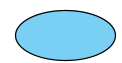
\includegraphics[width=0.1\linewidth]{images/ovalo.png}
    \end{minipage}
    \item Representa al actor que va a interactuar con el sistema.
    \begin{minipage}{0.2\textwidth}
        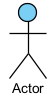
\includegraphics[width=0.1\linewidth]{images/actor.png}
    \end{minipage}
    \item Relación \texttt{<<extends>>}. Indica que un caso de uso puede ejecutarse a partir de otro.
    \item Relación \texttt{<<include>>}. Indica que un caso de uso debe ejecutarse a partir de otro.
\end{itemize}

La conexión entre un actor y un caso de uso se realiza mediante una línea como se muestra en la Figura 1.1.

\begin{figure}[htbp]
    \centering
    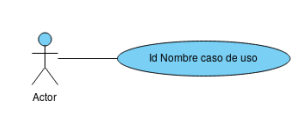
\includegraphics[width=0.4\textwidth]{images/interaccion.png}
    \caption{Interacción del actor con el caso de uso}
    \label{fig:interaccion-actor-caso-uso}
\end{figure}

Los casos de uso se encontrarán dentro de paquetes (representados por carpetas) indicando así que pertenecen a un mismo módulo, como se muestra en la Figura 1.2.

\begin{figure}[htbp]
    \centering
    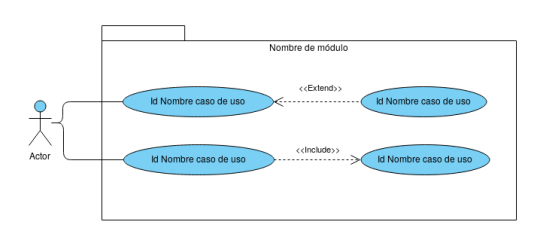
\includegraphics[width=0.6\textwidth]{images/interaccion2.png}
    \caption{Un Actor con varios casos de uso dentro de un módulo}
    \label{fig:actor-varios-casos-uso-modulo}
\end{figure}


%---------------------------------------------------------
\subsection{ Modelado Dinámico.}

Se centra en capturar y representar el comportamiento y las interacciones del sistema a lo largo del tiempo. Se utiliza para describir cómo los diferentes componentes del sistema interactúan entre sí y cómo se llevan a cabo las acciones y procesos. El modelado dinámico se realiza mediante diagramas de secuencia, diagramas de actividad, diagramas de estado y otras técnicas que permiten visualizar y analizar el flujo de eventos y el comportamiento dinámico del sistema.




%---------------------------------------------------------
\subsection{Modelos de Manejo de la Información}
Los modelos de manejo de la información se refieren a la representación y estructuración de los datos que serán almacenados y manipulados por el sistema. Estos modelos describen las entidades, atributos y relaciones entre los datos, y pueden incluir diagramas de entidad-relación, diagramas de clase y otros diagramas que ayudan a visualizar y comprender la estructura de los datos. El diseño de los modelos de manejo de la información busca garantizar la integridad, consistencia y eficiencia en la gestión de los datos, así como la adaptación a las necesidades específicas del sistema de la guardería.

Al abordar estos temas en el diseño del sistema de la guardería, se busca establecer una arquitectura sólida, modular y eficiente, así como una gestión efectiva de la información. Estos elementos son fundamentales para garantizar el rendimiento, la escalabilidad y la usabilidad del sistema, y para satisfacer las necesidades y expectativas de los usuarios finales.

% ==========================================================
%=========================================================
\chapter{Modelo del Alcance}
\label{cap:reqUsr}

	En este capítulo se modela el alcance del sistema. Se presentan inicialmente los Actores involucrados y sus requerimientos, especificando cuales se alcanzaron en la primera iteración y cuales serán trabajados en la segunda iteración. Después se presentan los requerimientos funcionales de esta iteración y al final se presenta el modelo Físico y Lógico del sistema.


%---------------------------------------------------------


%---------------------------------------------------------
\section{Requerimientos}

\subsection{Requerimientos de Usuario}
	\begin{requerimientosU}
		\FUitem{RU1}{Conocer info de profesores}{Los      padres de familia deben poder visualizar la
            informacion de los profesores en el momento que lo requieran}{Alta}
		\FUitem{RU2}{Registro de niños}{Los profesores deben poder seleccionar a los niños para realizar el reporte de estos.}{Alta}
		\FUitem{RU3}{Registro de salas}{Se necesita poder asignar a los niños a las salas, visualizando la disponibilidad de las salas.}{Moderada}
		\FUitem{RU4}{Registro de menú}{Se necesita tener el registro de lo que los niños van a comer durante el mes, y que los padres lo puedan visualizar}{baja}
		\FUitem{RU5}{Registro de ingestas}{Se necesita tener registro de que tanto comieron los niños para que los padres puedan visualizarlo.}{Moderada}
            \FUitem{RU6}{Registro de evacuaciones}{Se necesita tener registro de las evacuaciones los niños para que los padres puedan visualizarlo.}{Moderada}
            \FUitem{RU7}{Registro de actividades}{Se necesita tener registro de las actividades realizadas por los niños para que los padres puedan visualizarlo.}{Baja}
            \FUitem{RU8}{Registro de actividades en casa}{Los profesores necesitan poder registrar las actividades que los niños tienen que hacer en casa para que los padres puedan enterarse.}{Baja}
            \FUitem{RU9}{Incidencias médicas}{Se necesita tener un registro de cada diagnostico que el doctor le realiza a un niño.}{Moderada}
            \FUitem{RU10}{Solicitud de material}{Los profesores necesitan registrar los materiales que se ocuparán en cada clase.}{Baja}
            \FUitem{RU11}{Eventos escolares}{La directora necesita registrar cuándo hay eventos escolares.}{Moderada}
            \FUitem{RU12}{Dias inhabiles}{La directora necesita registrar los días inhábiles.}{Baja}
            \FUitem{RU13}{Asistencia}{Se necesita registrar la asistencia de cada niño en cada grupo por su profesor.}{Moderada}
            \FUitem{RU14}{Cambios de ropa}{Los profesores necesitan registrar los cambios de ropa de los niños durante el día.}{Moderada}
            \FUitem{RU15}{Reportes}{En caso de alguna incidencia con alguno de los niños, el profesor debe hacer un reporte sobre lo ocurrido, se tiene que llevar un registro de estos reportes.}{Moderada}
            \FUitem{RU16}{Citas}{Los profezores y doctores necesitan agendar citas con los tutores responsables de cada niño.}{Baja}
            \FUitem{RU17}{Modificacion info-niños}{Capital Humano necesita poder modificar cualquier informacion de los niños inscritos a la guarderia en cualquier momento.}{Alta}
            \FUitem{RU18}{Modificacion info-profesores}{Recursos Humanos necesita poder modificar la informacion del personal de la guarderia en cualquier momento de forma rapida.}{Alta}
            \FUitem{RU19}{Permisos y autorizaciones}{Los padres necesitan dar de alta a dos personas mas responsables del niño, en caso de que ellos no puedan recoger al niño}{Alta}
            \FUitem{RU20}{Escalabilidad de usuarios}{El personal de la guarderia necesita consultar rapidamente la informacion de los niños, asi como la informacion de cualquier otro personal.}{Alta}
            \FUitem{RU21}{Asignacion de alumnos a salas}{Capital Humanos necesita asignar a cada niño a su grupo y salon correspondiente}{Moderada}
            \FUitem{RU22}{Asignar profesores a salas}{La guarderia necesita por cada salon a un profesor y dos auxiliares}{Moderada}
            \FUitem{RU23}{Acceso 24/7 a los reportes de los alumnos}{Se rquiere reformar la forma en la que los tutores acceden a los reportes de sus hijos, pudiendo ahora acceder en cualquier momento de la semana, sin restricciones horarias.}{Alta}
            
            \FUitem{RU24}{Acceso a los reportes}{Se mantendrá el acceso exclusivo de los padres a los reportes de sus hijos, sin la capacidad de realizar acciones de personal administrativo.}{Alta}
            \FUitem{RU25}{Sitio web}{La plataforma debe ser una página web con un diseño moderno, intuitivo y fácil de navegar para el usuario.}{Alta}
            \FUitem{RU26}{Registro padres}{El personal de servicios sociales llevara a cabo el registro de tutores de los ninos, este registro se realizara cada periodo de inscripciones/reinscripciones.}{Alta}
            \FUitem{Ru27}{Fotografias}{Se debe mantener el sistema actual de identificacion de ninos y tutores, por lo que se requiere guardar una fotografía de cada uno para su facil identificacion.}{Moderada}
            \FUitem{RU28}{Seguridad}{Se deben tomar medidas de seguridad para garantizar que la información de los padres y alumnos esté protegida contra accesos no autorizados o fugas de información.}{Moderada}
            \FUitem{RU29}{Interfaz de usuario facil de usar}{La plataforma debe ser fácil de usar, con una interfaz intuitiva que permita a cualquier usuario acceder a la información correspondiente de manera sencilla.}{Baja}
            \FUitem{RU30}{Estudio socioeconomico}{Se requerirá que los padres respondan unas preguntas simples para conocer su situación económica, sin la necesidad de completar formularios complejos o extensos.}{Baja}
	\end{requerimientosU}
    


%---------------------------------------------------------
\subsection{Requerimientos funcionales}
    \begin{requerimientos}
        \FRitem{RF1}{Registro profesores}{Recursos Humanos deberá ingresar el nombre, dirección, número de teléfono.}{Alta}{RU1}
        \FRitem{RF2}{Creacion usuario y contraseña profesor}{Una vez registrados los datos del profesor, el sistema le asignará un usuario y contraseña para que el profesor pueda acceder a las funciones de los profesores.}{Alta}{RU1}
        \FRitem{RF3}{Cambiar contraseña profesor}{El profesor podrá cambiar su contraseña ingresando la contraseña actual y su nueva contraseña.}{Alta}{RU1}
        \FRitem{RF4}{registro padres}{Capital humano deberá ingresar el nombre, dirección, número de teléfono.}{Alta}{RU26}
        \FRitem{RF5}{Creacion usuario y contraseña padre}{Una vez registrados los datos del profesor, el sistema le asignará un usuario y contraseña para que el profesor pueda acceder a las funciones de los padres.}{Alta}{RU26}
        \FRitem{RF6}{Cambiar contraseña padre}{El padre podrá cambiar su contraseña ingresando la contraseña actual y su nueva contraseña.}{Alta}{RU26}
        \FRitem{RF7}{Inicio sesion profesor}{Los profesores ingresarán su usuario y contraseña, entonces el sistema validará la existencia de ese usuario y de ser que exista, le otorgara su token de acceso. }{Moderada}{RU28}
        \FRitem{RF8}{Inicio sesion padre}{Los padres ingresarán su usuario y contraseña, entonces el sistema validará la existencia de ese usuario y de ser que exista, le otorgara su token de acceso.}{Moderada}{RU28}
        \FRitem{RF9}{Registro niños}{Capital humano deberá ingresar el nombre, dirección, edad.}{Alta}{RU2}
        \FRitem{RF10}{Enlazar padre-niño}{Capital humano asignará a cada padre de familia los niños de los que es \textquotedblleft responsable\textquotedblright .}{Alta}{RU19}
        \FRitem{RF11}{Registro salas}{Capital humano deberá ingresar el nombre, grado, y localización de una sala.}{Moderada}{RU3}
        \FRitem{RF12}{Registro nutriologo}{Capital humano deberá ingresar el nombre, dirección, cédula del nutriologo.}{Baja}{RU4}
        \FRitem{RF13}{Usuario y contraseña nutriologo}{Una vez registrados los datos del nutriólogo, el sistema le asignará un usuario y contraseña para que el profesor pueda acceder a las funciones del nutriólogo.}{Baja}{RU4}
        \FRitem{RF14}{Inicio sesión nutriologo}{El nutriólogo ingresará su usuario y contraseña, entonces el sistema validará la existencia de ese usuario y de ser que exista, le otorgara su token de acceso.}{Baja}{RU4}
        \FRitem{RF15}{Registro menú}{El nutriólogo ingresará las comidas de cada día hábil.}{Baja}{RU4}
        \FRitem{RF16}{Visualizacion menú mensual}{Los padres de familia podrán visualizar el menú del mes actual.}{Baja}{RU4}
        \FRitem{RF17}{Vsualizacion menú del día}{Al momento de que los padres de familia ingresen al sistema, se les mostrara el menú planeado para el dia actual.}{Baja}{RU4}
        \FRitem{RF18}{Viusalizacion menú día especifico}{Los padres de familia podrán seleccionar un dia del mes actual o de un mes pasado y visualizar el menú de ese dia.}{Baja}{RU4}
        \FRitem{RF19}{Registro de ingestas}{Los profesores podran seleccionar una sala y podran seleccionar uno de las opciones de ingesta de cada niño para cada comida.}{Alta}{RU5}
        \FRitem{RF20}{Registro de evacuaciones}{Los profesores podran seleccionar una sala y podran seleccionar uno de las opciones de evacuacion de cada niño y la cantidad de estas.}{Alta}{RU6}
        \FRitem{RF21}{Registro actividadees}{Los profesores podran seleccionar una sala y registrar que actividades realizaron con esa sala en el dia actual.}{Alta}{RU7}
        \FRitem{RF22}{Registro de actividades en casa}{Los profesores podran seleccionar una sala y registrar que actividades tienen que hacer los niños en sus casas.}{Alta}{RU8}
        \FRitem{RF23}{Visualizacion de actividades en casa}{Al entrar al sistema, los padres podran ver que actividades tienen que hacer con sus hijos para el siguiente dia.}{Alta}{RU8}
        \FRitem{RF24}{Registro medico}{Capital humano ingresará el nombre, dirección, telefono, cedula del médico.}{Alta}{RU9}
        \FRitem{RF25}{Asignacion usuario y contraseña medico}{Una vez registrados los datos del médico, el sistema le asignará un usuario y contraseña para que el profesor pueda acceder a las funciones del médico.}{Moderada}{RU9}
        \FRitem{RF26}{Inicio sesión medico}{El médico ingresará su usuario y contraseña, entonces el sistema validará la existencia de ese usuario y de ser que exista, le otorgara su token de acceso.}{Moderada}{RU9}
        \FRitem{RF27}{Registro incidencia medica}{El médico seleccionará a un niño y registrara la fecha y hora del incidente así como el incidente en si.}{Baja}{RU9}
        \FRitem{RF28}{Solicitud material}{Los profesores registraron el material que necesitan para la siguiente clase}{Baja}{RU10}
        \FRitem{RF29}{Visualización material}{Cuando los padres de familia accedan al sistema, se les mostrará un aviso con el material que deben de llevar para el siguiente día.}{Baja}{RU10}
        \FRitem{RF30}{Registro de eventos escolares}{El director seleccionará una fecha y registrará un evento para ese dia, ademas de la hora de inicio y fin del evento.}{Alta}{RU11}
        \FRitem{RF31}{Inicio sesión director}{El director ingresará su usuario y contraseña, entonces el sistema validará la existencia de ese usuario y de ser que exista, le otorgara su token de acceso.}{Alta}{RU11}
        \FRitem{RF32}{Visualización de eventos escolares}{El sistema contará con una sección de próximas fechas donde se mostrarán los siguientes eventos escolares.}{Alta}{RU11}
        \FRitem{RF33}{Detalle eventos escolares}{Los padres de familia podrán seleccionar un evento escolar de la sección de próximas fechas y visualiza los detalles del evento.}{Media}{RU11}
        \FRitem{RF34}{Registro de días inhabiles}{El director seleccionará una fecha y lo marcará como dia habil.}{Baja}{RU12}
        \FRitem{RF35}{Visualizacion días inhabiles}{El sistema contara con una sección de fechas importantes donde se mostraran los días inhábiles.}{Alta}{RU12}
        \FRitem{RF36}{Toma de asistencia}{El profesor podrá consultar una lista con todos los niños de sus salas asignadas y marcará que niños asistieron y a que hora ingresaron.}{Alta}{RU13}
        \FRitem{RF37}{Registrar salida}{El profesor podrá consultar una lista con todos los niños que se encuentran en su sala seleccionara uno y registrara su hora de salida.}{Alta}{RU13}
        \FRitem{RF38}{Registrar cambio de ropa}{El profesor registrará la ropa que los padres le entregan y a que niño le pertenece.}{Baja}{RU14}
        \FRitem{RF39}{Consulta ropa}{El sistema le mostrará al profesor cuantas mudas tiene un niño y el estado de estas mudas, mostrando un aviso cuando no queden mudas limpias.}{Baja}{RU14}
        \FRitem{RF40}{Registrar uso de ropa}{El profesor registrará el uso de una muda de ropa y el sistema removerá esa muda de la lista de mudas disponibles.}{Baja}{RU14}
        \FRitem{RF41}{Generar reporte diario infante}{El sistema generará un reporte de cada niño con la fecha del reporte, las ingestas del niño, sus evacuaciones, su hora de entrada y su hora de salida.}{Alta}{RU15}
        \FRitem{RF42}{Registro informacion adicional al reporte diario infante}{El profesor podrá seleccionar a un niño que pertenezca a una de sus salas asignadas y le registrara observaciones para incluirlo en el reporte diario.}{Moderada}{RU15}
        \FRitem{RF43}{Visualizar reporte}{Los padres de familia podrán seleccionar a uno de sus niños y veran el reporte diario del niño.}{Moderado}{RU15}
        \FRitem{RF44}{Generar cita con un padre}{El profesor seleccionará a un niño, una fecha y hora para solicitar un citatorio con algún encargado del niño.}{Baja}{RU16}
        \FRitem{RF45}{Medico solicita cita}{El médico seleccionará a un niño, una fecha y hora para solicitar un citatorio con algún encargado del niño}{Baja}{RU16}
        \FRitem{RF46}{Generar cita con profesor}{Los padres de familia seleccionarán una fecha y hora para solicitar un citatorio con los profesores asignados a la sala de uno de sus niños.}{Baja}{RU16}
        \FRitem{RF47}{Generar cita con medico}{Los padres de familia seleccionarán una fecha y hora para solicitar un citatorio con el médico.}{Baja}{RU16}
        \FRitem{RF48}{Visualizar cita padre}{El sistema contará con el apartado de citatorios, donde los padres de familia podrán visualizar todos los citatorios que han solicitado y todos los citatorios a los que le citaron.}{Baja}{RU16}
        \FRitem{RF49}{Visualizar cita profesor}{El sistema contará con el apartado de citatorios, donde los profesores podrán visualizar todos los citatorios que han solicitado y todos los citatorios a los que le citaron.}{Baja}{RU16}
        \FRitem{RF50}{Visualizar cita medico}{El sistema contará con el apartado de citatorios, donde los médicos podrán visualizar todos los citatorios que han solicitado y todos los citatorios a los que le citaron.}{Baja}{RU16}
        \FRitem{RF51}{Modificar datos infante}{Capital humano podrá actualizar los datos de los niños.}{Baja}{RU17}
    \end{requerimientos}


%---------------------------------------------------------
\subsection{Requerimientos no funcionales}
    \subsubsection{Requerimientos del negocio}
    \begin{NFRequerimientos}
        \NFRitem{RNF1}{Colores del establecimiento}{Los colores de las pantallas deberán ser los colores que usa.}{Alta}{RU25}
        \NFRitem{RNF2}{Roles dentro del negocio}{Al igual de en la guardería, existe una distribución en las personas encargadas en cada área del trabajo, y cada área se encarga de una tarea en específico.}{Alta}{RU1, RU2, RU3, RU4, RU5}
        \NFRitem{RNF3}{Niños en grupos especificos}{Un grupo de niños no puede tener más de 30 niños y se dividen en grupos por edad (Lactantes de 3 meses a 1 año, 1 - 2 años y Maternal hasta los 6 años)}{Alta}{RU3}
        \NFRitem{RNF4}{Menú guarderia}{El nutriólogo da hasta 4 menús diarios distintos y estos llegan a depender de notas hechas por los padres sobre el niño.}{Alta}{RU4}
        \NFRitem{RNF5}{Reporte de incidencias médicas}{El doctor no puede hacer recetas médicas, pero sí observaciones y evalúa al niño en cuanto surja un incidente y tiene que notificarle al tutor.}{Alta}{RU9}
        \NFRitem{RNF6}{Niños especiales}{Es posible aceptar a niños especiales dentro de la guardería, siempre y cuando toda su información correspondiente sea notificada antes de hacer su inscripción.}{Alta}{RU2}
        \NFRitem{RNF7}{Seguridad en el establecimiento}{Existen medidas implementadas para identificar correctamente a los niños con sus tutores y esto es mediante credenciales y conociendo una foto del tutor responsable que debe estar dentro del sistema.}{Alta}{RU7}
        \NFRitem{RNF8}{Horario de la guarderia}{No existe un tiempo definido para que los profesores escriban los reportes a los niños correspondientes.}{Moderada}{RU8}
        \NFRitem{RNF9}{Evaluacion y seguimiento del desarrollo del niño}{Se realizarán evaluaciones periódicas del desarrollo de los niños para identificar posibles problemas y garantizar que estén recibiendo la atención necesaria.}{Moderada}{RU6}
        \NFRitem{RNF10}{Comunicación con los padres}{Se mantendrá una comunicación constante con los padres, por medio de reuniones periódicas, para informarles sobre el desarrollo de sus hijos y cualquier incidente que surja en la guardería, ademas de avisos dentro del sistema.}{Moderada}{RU10}
        \NFRitem{RNF11}{Profesores encargados}{En cada sala debe haber tres profesores por turno asignados para cuidar al grupo.}{Baja}{RU1}
        \NFRitem{RNF12}{Profesores por turno}{La guardería cuenta con dos turnos, por lo que al cambio de turno, cambian los profesores a cargo del grupo.}{Baja}{RU1}
        \NFRitem{RNF13}{Encargados alumno}{cada niño es asignado a su padre de familia mas dos encargados que pueden pasar a recogerlo.}{Baja}{RU26}
        \end{NFRequerimientos}

        \subsubsection{Requerimientos de informacion y datos}
        \begin{NFRequerimientos}
        \NFRitem{RNF14}{Seguridad en almacenamiento de la informacion}{Debe ser un sistema seguro para mantener la información privada tanto de las personal de la guardería, como de los clientes.}{Alta}{RU28}
        \NFRitem{RNF15}{Seguridad en el acceso a la informacion}{No todos los miembros del personal tienen acceso a los mismos datos de los clientes.}{Alta}{RU28}
        \NFRitem{RNF16}{Seguridad de contraseñas}{Las contraseñas deben ser cifradas, dentro del sistema para que solamente los clientes de las guarderías puedan entrar.}{Moderada}{RU28}
        \NFRitem{RNF17}{Informacion correspondiente}{La información del cliente debe corresponder a solamente a él, y debe ser inaccesible para terceros.}{Alta}{RU28}
        \NFRitem{RNF18}{Almacenamiento}{Toda la información agregada al sistema debe poder ser guardada por más de 6 años, en el transcurso del tiempo puede ser modificada o alterada.}{Alta}{RU23}
        \NFRitem{RNF19}{Cedulas profesionales}{La cedula profesional de los profesores y de los doctores y nutriologas puede ser vista dentro de la página de la guardería para todos los tutores que esten en la guarderia.}{Baja}{RU1, RU9}
        \NFRitem{RNF20}{Copias de seguridad periodicas}{El sistema debe realizar copias de seguridad periódicas, para garantizar la disponibilidad de la información en caso de pérdida o daño al sistema.}{Alta}{RU23}
        \NFRitem{RNF21}{Registro de accesos y cambios}{El sistema debe llevar un registro de accesos y cambios realizados en la información para garantizar la trazabilidad y la seguridad de la información.}{Alta}{RU23, RU28}
        \NFRitem{RNF22}{Seguridad}{El sistema debe contar con medidas de seguridad para proteger la información de los usuarios y el acceso no autorizado a la plataforma.}{Alta}{RU28}
        \NFRitem{RNF23}{Pruebas de seguridad}{El sistema debe someterse periódicamente a pruebas de seguridad para detectar posibles fallos o vulnerabilidades en su funcionamiento.}{Moderada}{RU28}
        \NFRitem{RNF24}{Privacidad de datos}{El sistema debe respetar la privacidad de los datos de los usuarios y cumplir con las leyes de protección de datos personales.}{Alta}{RU28}
        \NFRitem{RNF25}{Actualizacion de software}{El sistema debe actualizar regularmente su software y parches de seguridad para garantizar la protección y seguridad de la información.}{Alta}{RU23, RU28}
        \NFRitem{RNF26}{Formato contraseña}{Las contraseñas deben de contener al menos una mayúscula, una minúscula y un número, además de tener una extensión de mínima de 8 caracteres.}{Baja}{RU28}
        \NFRitem{RNF27}{Manejo de tokens}{El sistema manejara tokens para controlar el acceso y estos se desactivarán después de un lapso de inactividad de 5 minutos.}{Baja}{RU28}
        \end{NFRequerimientos}


        \subsubsection{Requerimientos de interaccion con el usuario}
        \begin{NFRequerimientos}
        \NFRitem{RNF28}{Tiempo de acceso}{No debe de tomarle más de 5 segundos al usuario ingresar a su cuenta.}{Baja}{RU23}
        \NFRitem{RNF29}{Tiempo de interaccion}{No debera de tardar más de 5 segundos el usuario en hacer o recibir una solicitud de la página.}{Baja}{RU23}
        \NFRitem{RNF30}{Capacidad de respuesta}{El sistema debe responder de manera rápida y sin demora ante las acciones del usuario.}{Moderada}{RU20, RU23}
        \NFRitem{RNF31}{Disponibilidad con usuarios}{La aplicación debe estar disponible en todo momento, salvo en mantenimientos planificados.}{Alta}{RU1}
        \NFRitem{RNF32}{Accesibilidad de usuarios}{La aplicación debe ser accesible para todos los usuarios, incluyendo personas con discapacidades, mediante el uso de tecnologías de apoyo.}{Alta}{RU12}
        \NFRitem{RNF33}{Estabilidad de usuarios}{La aplicación debe ser estable y no presentar errores críticos que afecten su funcionamiento.}{Alta}{RU1, RU20, RU23}
        \NFRitem{RNF34}{Valores}{Todas las paginas deben estar escritas correctamente con respeto a los usuarios}{Baja}{RU1}
        \NFRitem{RNF35}{Mensajes limitantes}{Los usuarios pueden mandar mensajes directos a subdirección si tienen dudas específicas.}{Baja}{RU1}
        \NFRitem{RNF36}{Notificaciones}{Las notificaciones deben llegar al correo electronico de los tutores y al celular como un mensaje.}{Baja}{RU1, RU20, RU23}
        \NFRitem{RNF37}{Tipos salidas}{La salida de datos debe ser visualizada en una pantalla.}{Alta}{RU1}
        \NFRitem{RNF38}{Inputs}{La aplicación debe funcionar sin nuevos dispositivos de entrada, mas que el teclado y mouse.}{Alta}{RU1}
        \end{NFRequerimientos}

        \subsubsection{Requerimientos de plataforma}
        \begin{NFRequerimientos}
        \NFRitem{RNF39}{Plataforma del sistema}{El sistema debe ser capaz de correr desde una computadora en un navegador web, como en un celular.}{Alta}{RU23}
        \NFRitem{RNF40}{Escalabilidad dentro del sistema}{El sistema debe tener la capacidad de ir creciendo, conforme crece el negocio.}{Alta}{RU20}
        \NFRitem{RNF41}{Disponibilidad del sistema}{El sistema debe estar disponible las 24 horas del día todos los días de la semana, en caso de hacer mantenimiento este no deberá dejar el servicio por máximo 30 minutos.}{Alta}{RU23}
        \NFRitem{RNF42}{Integración con otras herramientas}{El sistema debe poder integrarse con otras herramientas o software utilizados por la organización, para mejorar el flujo de trabajo y la eficiencia del negocio.}{Moderada}{RU19}
        \NFRitem{RNF43}{Escalabilidad en la base de datos}{La base de datos del sistema debe ser escalable para soportar un gran volumen de datos sin perder rendimiento.}{Moderada}{RU20}
        \NFRitem{RNF44}{Interfaz del usuario intuitiva}{La interfaz de usuario del sistema debe ser fácil de usar y entender para cualquier tipo de usuario.}{Moderada}{RU22}
        \NFRitem{RNF45}{Compatibilidad con diferentes navegadores}{El sistema debe ser compatible con los navegadores más utilizados como Chrome, Firefox, Safari y Edge.}{Moderada}{RU23}
        \NFRitem{RNF46}{Capacidad de exportar datos}{El sistema debe permitir la exportación de datos en diferentes formatos para realizar análisis externos y generar informes personalizados.}{Moderada}{RU21}
        \NFRitem{RNF47}{Multidispositivo}{La aplicación debe ser compatible y adaptarse a diferentes dispositivos, como ordenadores, smartphones y tablets.}{Alta}{RU14}
        \end{NFRequerimientos}

        \subsubsection{Requerimientos de propiedades de software}
        \begin{NFRequerimientos}
        \NFRitem{RNF48}{Sistema amigable}{Debe ser fácil para los usuarios interactuar con el sistema, y que les parezca intuitivo manejarlo.}{Baja}{RU29}
        \NFRitem{RNF49}{Calidad dentro del proyecto}{Debe ser atractivo visualmente todas las páginas del sistema.}{Baja}{RU29}
        \NFRitem{RNF50}{Confiabilidad}{El sistema debe estar libre de bugs o errores al momento de ser desplegado para no interferir con la experiencia del usuario.}{Alta}{RU29}
        \NFRitem{RNF51}{Mantenibilidad}{El sistema puede ser modificado dentro del tiempo que es usado, por decisión de los stakeholders, además de que pueda ser transparente(Ningún cambio afecte el funcionamiento del sistema ni de su información ya almacenada).}{Moderada}{RU25}
        \NFRitem{RNF52}{Estabilidad}{No puede caerse el sistema si hay una gran cantidad de usuarios activos en el momento de operación, ni afectar su desempeño.}{Moderada}{RU20}
        \NFRitem{RNF53}{Privacidad}{Debe de mantenerse privada la información personal de todos los usuarios ante terceros, además solo la podrán ver personal específico de la guardería.}{Alta}{RU28}
        \NFRitem{RNF54}{Seguridad}{El sistema debe contar con medidas de seguridad para proteger la información almacenada en él, como cifrado de datos y autenticación de usuarios.}{Alta}{RU28}
        \NFRitem{RNF55}{Escalabilidad}{El sistema debe ser capaz de crecer y aumentar su capacidad de manejo de usuarios e información de manera eficiente y sin comprometer su rendimiento.}{Moderada}{RU20}
        \NFRitem{RNF56}{Documentacion}{El sistema debe contar con una documentación adecuada que permita comprender su funcionamiento y facilitar su mantenimiento por parte de los desarrolladores.}{Baja}{RU25}
        \NFRitem{RNF57}{Tamaño fotos}{El sistema redimensiona las fotos de los encargados de los niños a 500 px x 400px.}{Baja}{RU27}
        \NFRitem{RNF58}{Responsivo}{La página web del sistema debe de ser responsiva.}{Baja}{RU29}
        \NFRitem{RNF59}{Host}{El sistema debe estar hosteado en un dominio .com}{Baja}{RU25}
        \NFRitem{RNF60}{BD}{La base de datos de datos debe de estar hosteada en un servidor.}{Baja}{RU25}
        
    \end{NFRequerimientos}

    
%---------------------------------------------------------
\section{Especificación de plataforma}	
	
\begin{description}
	\item[Tipo de sistema:] Nuestro sistema se implementara con una aplicación web.
	\item[Software requerido:] Para el funcionamiento de la aplicacion web se requiere lo siguiente:
        \begin{itemize}
            \item {\bf Sistema operativo}:Compatible con Windows, macOS y Linux
            \item {\bf Navegador web}:
            \item {\bf Servidor}:
            \item {\bf Lenguajes de programacion}:
            \item {\bf Frameworks}:
            \item {\bf Base de datos}:
            \item {\bf IDE}: Se recomienda el uso de Visual Studio Code para el desarrollo
        \end{itemize}
	\item[Hardware requerido:] Para un renimiento optimo se recomienda el siguiente hardware
        \begin{itemize}
            \item {\bf CPU}:Intel core i5 8th Gen o equivalente
            \item {\bf Memoria RAM}:Minimo 4 GB
            \item {\bf Espacio en disco}: Al menos 5 GB de espacio disponible
            \item {\bf Conexion a Internet}:Se requiere de una conexion estable para garantizar el acceso a la aplicacion.
        \end{itemize}
	\item[servicios:] Se recomienda que se cuente con los siguientes servicios:
        \begin{itemize}
            \item Conexión a internet estable y de alta velocidad para asegurar la disponibilidad del sistema.
            \item Respaldo de energía para evitar interrupciones con el servicio de la aplicación
            \item Medidas de seguridad para prevenir accesos no autorizados
        \end{itemize}
\end{description}


\begin{figure}[htbp!]
	\begin{center}
		\fbox{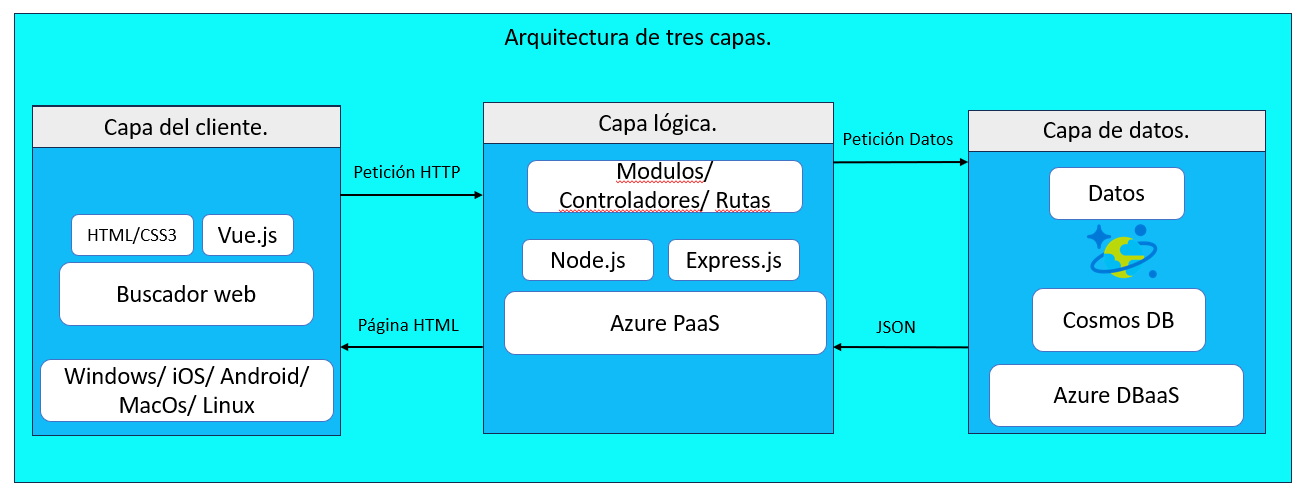
\includegraphics[width=.6\textwidth]{images/arqui/3capas}}
		\caption{Arquitectura del sistema.}
		\label{fig:arquitectura}
	\end{center}
\end{figure}

En la figura~\ref{fig:arquitectura} se describe la estructura del sistema.


%=========================================================
%=========================================================
\chapter{Modelo del Negocio}	
\label{cap:reqSist}

	En este capítulo se modela la {\em Arquitectura del negocio} la cual está conformada por la Ontología del negocio ({\em Términos} y {\em Hechos del negocio}), Arquitectura de procesos y las {\em Reglas del negocio}. Primero se especifica brevemente el {\em Contexto} en el que los términos tienen significado.
	
	En las secciones \ref{sec:terminosDeNegocio} y \ref{sec:hechosDeNegocio} se presentan los Términos del negocio a manera de Glosario y por último se presentan los Hechos del negocio a manera de relaciones entre términos del negocio.

%----------------------------------------------------------
\section{Contexto}

	La empresa ``Guarderia Burbujas'' se dedica a el cuidado y atencion de infantes. Su principal objetivo es brindar un entorno seguro, educativo y estimulante para el desarrollo integral de los niños mientras sus padres trabajan o realizan otras actividades.
    La guarderia cuenta con salas en donde se quedan los infantes, mientras tres docentes los estan cuidando y realizando actividades con ellos, si alguninfante tiene que ir a hacer una evacuacion un profesor lo acompaña y los otros dos se quedan vigilando a los demas infantes.
    Tambien se cuenta con un nutriologo en cargado de mantener a los infantes con una dieta balanceada y con un medico engargado de atender cualquier incidente medico que ocurra dentro de la guarderia.
	
%---------------------------------------------------------
\section{Términos del Negocio}
\label{sec:terminosDeNegocio}

\begin{description}
	\item[\hypertarget{tusuario}{Usuario:}] Persona fisica que tienen acceso al sistema. 
 
	\item[\hypertarget{tinfante}{Infante:}] Se refiere a las personad de entre 3 meses y 6 años que asisten a la guarderia.
	
	\item[\hypertarget{tDocente}{Profesor:}] Tipo de Usuario que esta al frente de una sala para cuidar a los infantes y dejarles actividades ludicas, asi como para estar al pendiente de sus ingestas y evacuaciones.
 
	\item[\hypertarget{treporte}{Reporte:}] Documento con el cual se le informa a los padres de familia las actividades que ha realizado su hijo durante el dia, como sus ingestas, evacuaciones y si hubo alcun incidente con su hijo.
	
	\item[\hypertarget{tEvento}{Evento:}] Acontecimientos relevantes en la guarderia como festivales, convivios o dias inhabiles.
	
	\item[\hypertarget{ttarea}{Tarea:}] Actividad que los profesores dejan a los infantes para que las realicen en casa con el proposito de reforzar lo visto en la guarderia. 

	\item[\hypertarget{tactividad}{Actividad:}] Se refiere a toda accion que el profesor solicita a los infantes que realicen durante su estandia en la guarderia con proposito educativo y que favorece el desarrollo del infante.
	
	\item[\hypertarget{tMenu}{Menu:}] Documento en el cual se puede visualizar las comidas de todo un mes de los infantes.

        \item[\hypertarget{tIngesta}{Ingesta:}] Material alimenticio o líquidos que se incorporan al organismo por la boca en un periodo determinado.

        \item[\hypertarget{tEvacuacion}{Evacuacion:}] Materia compuesta de residuos de alimento que el organismo elimina tras haber hecho la digestión.
        
        \item[\hypertarget{tNutriologo}{Nutriologo:}] Usuario encargado de hacer la planificacion del menu de los infantes, cuidando que tengan una dieta balanceada.
        
	
        \item[\hypertarget{tSala}{Sala:}] Lugar en la guarderia destinado a los infantes.

        
        \item[\hypertarget{tpadre}{Padre de familia:}] Engargado legal de un infante.

        
        \item[\hypertarget{tMedico}{medico:}] Usuario con licencia medica que Se encarga de atender temas de salud de los infantes.

        
        \item[\hypertarget{tdirector}{Director:}] Autoridad de la guarderia, se encarga de organizar los eventos escolares y los dias inhabiles.
        
%	\brTermSensor{tVelocimetro}{Velocímetro:}{Velocidad de un Vehículo.}{Kilometros/hora.}{Constantemente siempre que el \cdtRef{tVehiculo}{vehículo} esté encendido.}
\end{description}


\newpage
%----------------------------------------------------------
\section{Modelo del dominio del problema}
\label{sec:hechosDeNegocio}


%- - - - - - - - - - - - - - - - - - - - - - - - - - - - - 
\subsection{Modelo del dominio del problema}

	El modelo del dominio del problema se muestra en la figura~\ref{fig:modeloDeDominio}, a continuación se describen cada una de las entidades y sus relaciones.
	
\begin{figure}[htbp!]
	\begin{center}
		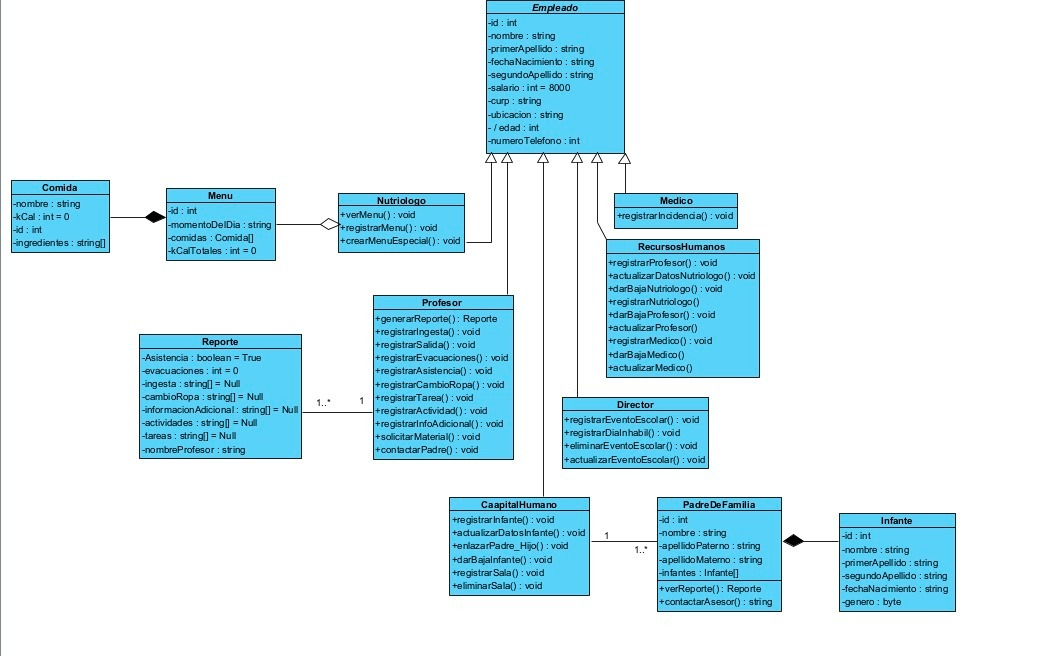
\includegraphics[angle=90,width=.58\textwidth]{images/diagramaClases.jpeg}
		\caption{Modelo del dominio del problema}
		\label{fig:modeloDeDominio}
	\end{center}
\end{figure}


\newpage
\begin{cdtEntidad}{infante}{Infante}
	\brAttr{id}{Id}{Id}{Número de registro utilizado para identificar un alumno}{Sí}
	\brAttr{nombre}{Nombre}{Palabra Corta}
		{Nombre o nombres del alumno.}{Sí}
	\brAttr{primerApellido}{Primer apellido}{Palabra Corta}
		{Primer apellido del alumno.}{Sí}
	\brAttr{segundoApellido}{Segundo apellido}{Palabra Corta}
		{Segundo apellido del alumno.}{No}
	\brAttr{nacimiento}{FechaNacimiento}{Fecha}
		{Fecha de nacimiento del alumno.}{Sí}
	\brAttr{genero}{Género}{byte}
		{Género del alumno.}{No}
\end{cdtEntidad}

%- - - - - - - - - - - - - - - - - - - - - - - - - - - - - 
\begin{cdtEntidad}{padredefamilia}{Padre de Familia}%{}
	\brAttr{id}{Id}{Id}{Número de registro utilizado para identificar un alumno}{Sí}
	\brAttr{nombre}{Nombre}{Palabra Corta}
		{Nombre o nombres del alumno.}{Sí}
	\brAttr{primerApellido}{Primer apellido}{Palabra Corta}
		{Primer apellido del alumno.}{Sí}
	\brAttr{segundoApellido}{Segundo apellido}{Palabra Corta}
		{Segundo apellido del alumno.}{No}
	\brAttr{infantes}{Infantes}{Lista}
		{Lista de todos los infantes a su cargo.}{Sí}
	\brAttr{reportes}{Reportes}{Lista}
		{Lista de todos los reportes de los infantes que tiene a cargo el padre de familia.}{No}
        \brAttr{citas}{Citas}{Lista}{Lista de todas las citas que tiene el padre de familia}{No}
	\cdtEntityRelSection
	\brRel{\brRelComposition}{Infante}{Un \hyperlink{padredefamilia}{Padre de familia} tiene \hyperlink{infante}{Infantes} a su cargo}	
	\brRel{\brRelComposition}{Citas}{Un \hyperlink{padredefamilia}{Padre de familia} tiene  \hyperlink{citas}{citas} a las que asistir}
        \brRel{\brRelComposition}{Reporte}{un \hyperlink{padredefamilia}{Padre de familia} tiene los \hyperlink{reporte}{reportes} de sus infantes}
\end{cdtEntidad}

%---------------------------------------------------------
\newpage
\begin{cdtEntidad}{citas}{Citas}
	\brAttr{fecha}{Fecha}{Fecha}{Fecha en la que la cita esta programada}{Sí}
	\brAttr{nombreinfante}{NombreInfante}{Palabra Corta}
		{Nombre del alumno.}{Sí}
	\brAttr{nombrepadre}{NombrePadre}{Palabra Corta}
		{nombre del padre del infante.}{Sí}
	\brAttr{hora}{Hora}{time}
		{Hora en la que la cita esta programada.}{Si}
	\brAttr{id}{ID}{byte}
		{Numero de registro utilizado para identificar la cita.}{Sí}
\end{cdtEntidad}

%- - - - - - - - - - - - - - - - - - - - - - - - - - - - - 
\begin{cdtEntidad}{Reportes}{Reportes}
	\brAttr{asistencia}{Asistencia}{Boolean}{muestra si el infante asistio un dia}{Sí}
	\brAttr{evacuaciones}{Evacuaciones}{Int}
		{muestra la cantidad de veces que el infante evacuó.}{Sí}
	\brAttr{ingesta}{Ingesta}{Palabra Corta}
		{Muestra la cantidad de comida que ingirio el infante.}{Sí}
	\brAttr{cambioropa}{CambioRopa}{Palabra Corta}
		{Muestra cuantos cambios de ropa uso el infante y cuantos tiene aun disponibles.}{No}
	\brAttr{informacionadicional}{Informacion Adicional}{String}
		{Muestra otra informacion que se considere relevante sobre el infante.}{Sí}
	\brAttr{actividades}{Actividades}{String}
		{Muestra las actividades realizadas por el alumno.}{No}
        \brAttr{tareas}{Tareas}{String}{Muestra las tareas que debe realizar el padre de familia con el infante}{No}
        \brAttr{nombreprofesor}{Nombre Profesor}{palara corta}{Muestra el nombre del profesor que realizo el reporte}{Si}
\end{cdtEntidad}

%- - - - - - - - - - - - - - - - - - - - - - - - - - - - - 
\begin{cdtEntidad}{comida}{Comida}
	\brAttr{nombre}{Nombre}{Palabra corta}{nombre del platillo}{Sí}
	\brAttr{kcal}{Kcal}{Int}
		{muestra la cantidad de kilo calorias que el platillo aporta.}{Sí}
	\brAttr{ingredientes}{Ingredientes}{String}
		{Muestra los ingredientes con los que se prepara una comida.}{No}
	\brAttr{id}{Id}{int}
		{Numero de registro con el que se identifica al platillo.}{Sí}
\end{cdtEntidad}
%- - - - - - - - - - - - - - - - - - - - - - - - - - - - - 
\newpage
\section{Modelado de Reglas de negocio}

\begin{BussinesRule}{RN1}{Fecha de Nacimiento correcta.}
	\BRitem[Tipo:] Regla de integridad referencial o estructural. 
				% Otras opciones para tipo: 
				% - Regla de integridad referencial o estructural. 
				% - Regla de operación, (calcular o determinar un valor.).
				% - Regla de inferencia de un hecho.
	\BRitem[Clase:] Habilitadora. 
				% Otras opciones para clase: Habilitadora, Cronometrada, Ejecutive.
	\BRitem[Nivel:] Control. % Otras opciones para nivel: Control, Influencia.
	\BRitem[Descripción:]	Las Fechas de Nacimiento de los infantes debe ser mayores al día Primero de Enero del año 2018 y menor a tres meses antes de la fecha actual.
	\BRitem[Motivación:] Evitar fraudes al PRONIM por el registro de personas que no han nacido al momento de su registro.
	\BRitem[Sentencia:] $\forall p \in Persona \Rightarrow 01-Enero-2018~<~p.fechaDeNacimiento~<~fechaActual menos 3 meses$.
	\BRitem[Ejemplo positivo:] Para el día 23 de Junio del 2023, cumplen la regla: 		
        \begin{itemize}
        	\item 11 de Octubre del 2020
			\item 20 de Diciembre del 2021
			\item 2 de Enero del 2023
        \end{itemize}
	
	\BRitem[Ejemplo negativo:] Para el día 23 de Junio del 2013, no cumplen la 
		\begin{itemize}
        	\item 12 de junio del 2013
			\item 20 de Diciembre del 2014
			\item 1 de Enero del 1900
			\item 31 de Diciembre del 2024
        \end{itemize}
	
	\BRitem[Referenciado por:] \hyperlink{CU3}{CU3}.
\end{BussinesRule}

\begin{BussinesRule}{RN2}{Atencion medica.} 
	\BRitem[Tipo:] Regla de Condicion. 
				% Otras opciones para tipo: 
				% - Regla de integridad referencial o estructural. 
				% - Regla de operación, (calcular o determinar un valor.).
				% - Regla de inferencia de un hecho.
	\BRitem[Clase:] Habilitadora. 
				% Otras opciones para clase: Habilitadora, Cronometrada, Ejecutive.
	\BRitem[Nivel:] Control. % Otras opciones para nivel: Control, Influencia.
	\BRitem[Descripción:] Cuando un infante requiera atencion medica de bajo nivel , el medico debe atenderlo de manera oportina, ademas de registrar el reporte de la incidencia medica.
        \BRitem[Motivación:] Garantiza el cuidado oportuno de los infantes, ademas de que notifica a los padres de familia cuando ocurre algo con sus hijos.
	\BRitem[Ejemplo positivo:] 
                \begin{itemize}
                    \item Juan se resbaló en el ultimo escalon, por lo que golpeo su cabeza, por lo que fue revisado por el medico para descartar una contucion y registra el reporte del incidente.
                \end{itemize}
	\BRitem[Ejemplo negativo:] 
                \begin{itemize}
                    \item Pedro se cayo y se raspo la rodilla, por lo que el medico le lavo la herida pero no realizo el reporte
	        \end{itemize}
         
	\BRitem[Referenciado por:] \hyperlink{CU15}{CU15}.
\end{BussinesRule}

\begin{BussinesRule}{RN3}{Notificacion de tareas}
	\BRitem[Tipo:] Regla de condicion.
				% Otras opciones para tipo: 
				% - Regla de integridad referencial o estructural. 
				% - Regla de operación, (calcular o determinar un valor.).
				% - Regla de inferencia de un hecho.
	\BRitem[Clase:] Habilitadora. 
				% Otras opciones para clase: Habilitadora, Cronometrada, Ejecutive.
	\BRitem[Nivel:] Influencia. % Otras opciones para nivel: Control, Influencia.
	\BRitem[Descripción:] Es responsabilidad del profesor dar a conocer las tareas que deberan hacer los infantes en sus casas para reforzar lo visto en el dia.
 
        \BRitem[Motivacion] Aumentar el desarrollo de los infantes, ademas de tener una buena comunicacion entre profesores y padres de familia
        
	\BRitem[Ejemplo positivo:] 
                \begin{itemize}
                    \item el profesor moises notifica a los padres de familia sobre todas las actividades que requiere que los infantes realicen en sus casa
                \end{itemize}
	
	\BRitem[Ejemplo negativo:] 
                \begin{itemize}
                    \item El profesor humberto no realiza la notificacion de tareas de los infantes, lo cual podria dificultar el progreso de los infantes
                \end{itemize}
 
	\BRitem[Referenciado por:] \hyperlink{CU12}{CU12}.
\end{BussinesRule}

\begin{BussinesRule}{BR4}{Toma de asistencia}
	\BRitem[Tipo:] Regla de integridad referencial o estructural.
				% Otras opciones para tipo: 
				% - Regla de integridad referencial o estructural. 
				% - Regla de operación, (calcular o determinar un valor.).
				% - Regla de inferencia de un hecho.
	\BRitem[Clase:] Habilitadora. 
				% Otras opciones para clase: Habilitadora, Cronometrada, Ejecutive.
	\BRitem[Nivel:] Control. % Otras opciones para nivel: Control, Influencia.
	\BRitem[Descripción:] Todos los profesores deberan tomar asistencia de los infantes todos los dias.
        \BRitem[Motivacion] Tener un control de cuando asistieron los infantes para poder mostrarlo a los padres de familia en caso de que se requiera
        
	\BRitem[Ejemplo positivo:] 
            \begin{itemize}
                \item El profesor ricardo pasa asistencia todos los dias a las 9:15
            \end{itemize}
	
	\BRitem[Ejemplo negativo:] 
	       \begin{itemize}
	           \item  El profesor humberto no pasa lista en la guarderia, pero cuando llega a su casa anota a los alumnos que recuerda que estuvieron.
	       \end{itemize}
	\BRitem[Referenciado por:] \hyperlink{CU19}{CU19} 
\end{BussinesRule}

\begin{BussinesRule}{RN5}{Asignacion de salas por edad}
	\BRitem[Tipo:] Regla de inferencia.
				% Otras opciones para tipo: 
				% - Regla de integridad referencial o estructural. 
				% - Regla de operación, (calcular o determinar un valor.).
				% - Regla de inferencia de un hecho.
	\BRitem[Clase:] Habilitadora. 
				% Otras opciones para clase: Habilitadora, Cronometrada, Ejecutive.
	\BRitem[Nivel:] Control. % Otras opciones para nivel: Control, Influencia.
	\BRitem[Descripción:] Los infantes seran asignados a salas basados en rangos de edades.
        \BRitem[Motivacion] Que los infantes tengan una buena interaccion social.
		
	\BRitem[Ejemplo positivo:] 
	        \begin{itemize}
	            \item Juanito de 7 meses fue asignado a una sala con infantes de 3 meses a 1 año 
	        \end{itemize}
	\BRitem[Ejemplo negativo:] 
	        \begin{itemize}
	            \item Juanito de 2 años fue asignado a una sala con infantes de 6 años
	        \end{itemize}
	\BRitem[Referenciado por: ]CU3 
\end{BussinesRule}

\begin{BussinesRule}{RN6}{Informar cantidad de ingesta}
	\BRitem[Tipo:] Inferencia de un hecho.
				% Otras opciones para tipo: 
				% - Regla de integridad referencial o estructural. 
				% - Regla de operación, (calcular o determinar un valor.).
				% - Regla de inferencia de un hecho.
	\BRitem[Clase:] Habilitadora. 
				% Otras opciones para clase: Habilitadora, Cronometrada, Ejecutive.
	\BRitem[Nivel:] Control. % Otras opciones para nivel: Control, Influencia.
	\BRitem[Descripción:] Los profesores deben de realizar el reporte de las cantidades de comida ingeridas por los infantes.
        \BRitem[Motivacion] Que los padres de familia esten informados acerca de la alimentacion de sus hijos
	\BRitem[Ejemplo positivo:] 
	        \begin{itemize}
	            \item El profesor alexis revisa cuanta comida queda en los platos de los infantes y anota cuanto comio cada quien, posteriormente registra las cantidades de comida ingeridas por los niños
	        \end{itemize}
	\BRitem[Ejemplo negativo:] 
	        \begin{itemize}
	            \item El profesor horacio no revisa cuanto come cada niño, y cuando le solicitan el reporte de ingestas registra que todos los niños acabaron toda su comida.
	        \end{itemize}
	\BRitem[Referenciado por:]CU9 
\end{BussinesRule}

\begin{BussinesRule}{RN7}{Informacion sobre eventos en la guarderia.}
	\BRitem[Tipo:] Regla de integridad.
				% Otras opciones para tipo: 
				% - Regla de integridad referencial o estructural. 
				% - Regla de operación, (calcular o determinar un valor.).
				% - Regla de inferencia de un hecho.
	\BRitem[Clase:] Habilitadora. 
				% Otras opciones para clase: Habilitadora, Cronometrada, Ejecutive.
	\BRitem[Nivel:] Control. % Otras opciones para nivel: Control, Influencia.
	\BRitem[Descripción:] El director debe notificar de todos los eventos academicos planeados a los padres de familia con al menos dos semanas de antelacion:
		
	\BRitem[Motivacion:] Que los padres de familia esten notificados de los eventos, teniendo sufuciente tiempo para saber si van a poder asistir, asi como de conseguir los materiales que se requieran.
	\BRitem[Ejemplo positivo:] 
	        \begin{itemize}
	            \item El director de la guarderia notifico el dia 21 de marzo que para el dia 10 de mayo se planea hacer un festival por el dia de las madres.
	        \end{itemize}
	\BRitem[Ejemplo negativo:] 
	        \begin{itemize}
	            \item El director de la guarderia notifica el 10 de septiembre que el dia 16 de septiembre tienen planeado realizar una kermes por el dia de la independencia
	        \end{itemize}
	\BRitem[Referenciado por:] CU17 
\end{BussinesRule}



%---------------------------------------------------------


%=========================================================
%=========================================================
\chapter{Modelo dinámico}	
\label{cap:modDinamico}

	Este capítulo describe en modelo dinámico del sistema. en el se detallan todos los escenarios de ejecución del sistema. La figura~\ref{fig:casosDeUso} muestra el diagrama general del sistema y sus sib sistemas, y la figura~\ref{fig:casosDeUsoDetalle} muestra todos los casos de uso del sistema. En este documento solo detallamos los casos de uso del subsistema de gestión de cursos.
	
\begin{figure}[htbp]
	\begin{center}
		\fbox{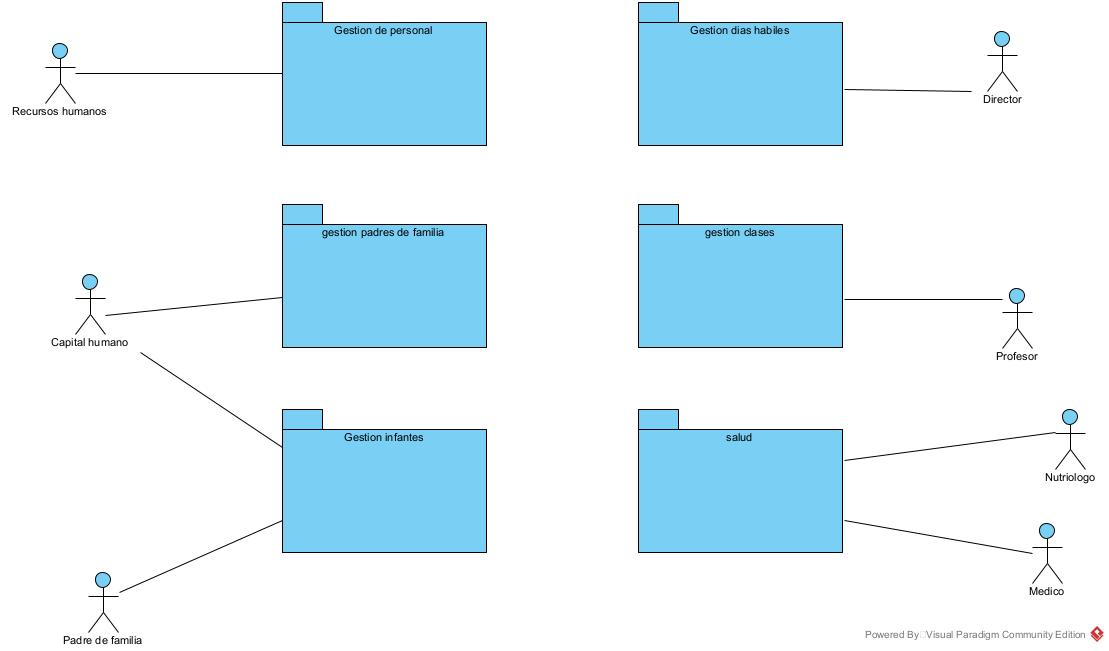
\includegraphics[width=.8\textwidth]{images/casosDeUso}}
		\caption{Diagrama de casos de uso del sistema.}
		\label{fig:casosDeUso}
	\end{center}
\end{figure}

\begin{figure}[htbp]
	\begin{center}
		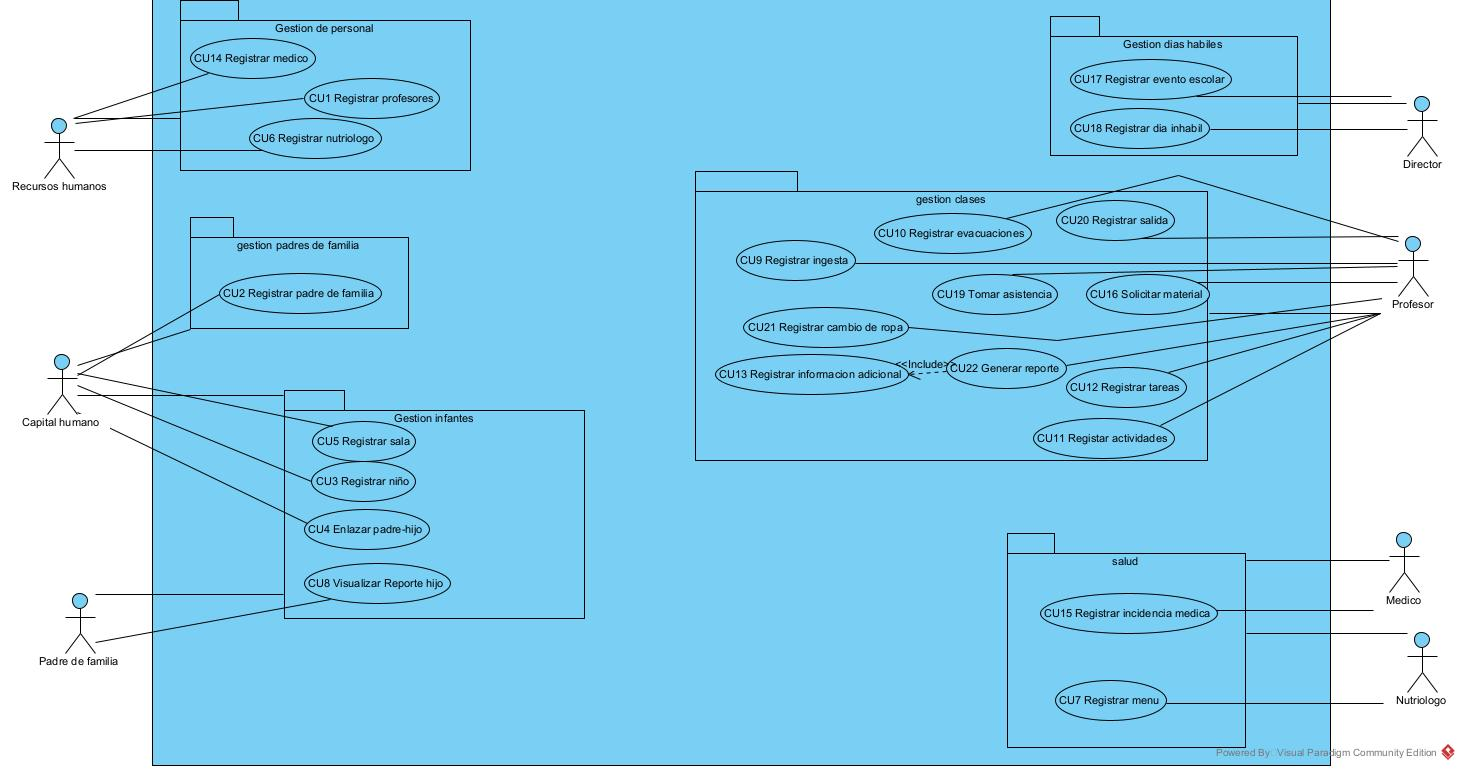
\includegraphics[angle=90, width=.7\textwidth]{images/casosDeUsoDetalle}
		\caption{Diagrama detallado del sistema.}
		\label{fig:casosDeUsoDetalle}
	\end{center}
\end{figure}

%---------------------------------------------------------
\section{Descripción de actores}

%---------------------------------------------------------
\begin{Usuario}{\hypertarget{recursosHumanos}{\subsection{Recursos humanos}}}{
	Es el responsable de la gestion del personal dentro de la guarderia.
}
    \item[Responsabilidades:] \cdtEmpty
    \begin{itemize}
		\item Administrar la contratacion y despido del personal
		
    \end{itemize}

	\item[Perfil:] \cdtEmpty
    \begin{itemize}
		\item Licenciatura en recursos humanos, administracion de empresas o afin.
		\item un año de experiencia minimo en gestion de recursos humanos.
		\item Habilidades de liderazgo y trato humano.
    \end{itemize}
\end{Usuario}

\begin{Usuario}{\hypertarget{capitalHumano}{\subsection{Capital humano}}}{
	Es el encargado de la inscripcion de los infantes, asi como de recolectar la informacion de sus padres de familia
}
    \item[Responsabilidades:] \cdtEmpty
    \begin{itemize}
		\item Gestionar los expedientes de los infantes.
		\item Gestionar el estatus del infante dentro de la guarderia.
		\item Es el enlace entre los padres de familia y la guarderia.
    \end{itemize}

	\item[Perfil:] \cdtEmpty
    \begin{itemize}
		\item Licenciatura en trabajo social o afin.
		\item Experiencia en la gestion de documentacion de personas, preferiblemente ede               infantes.
		\item Tener un buen trato con las personas.
    \end{itemize}
\end{Usuario}

\begin{Usuario}{\hypertarget{medico}{\subsection{Médico}}}{
	Es el encargado de mantener la salud y el bienestar de los infantes en la guarderia.
}
    \item[Responsabilidades:] \cdtEmpty
    \begin{itemize}
		\item Supervisar la salud de los infantes.
		\item Proporcionar atencion medica a los infantes en caso de algun incidente.
		\item Proporcionar informacion sobre la salud de los infantes a sus padres.
    \end{itemize}

	\item[Perfil:] \cdtEmpty
    \begin{itemize}
		\item Titulo en medicina, preferiblemente con especialidad en pediatria.
		\item Licencia medica valida.
    \end{itemize}
\end{Usuario}

\begin{Usuario}{\hypertarget{nutriologo}{\subsection{Nutriologo}}}{
	Es el encargado de la buena alimentacion de los infantes.
}
    \item[Responsabilidades:] \cdtEmpty
    \begin{itemize}
		\item Diseñar un plan alimenticio para los infantes que sea saludable.
		\item Dar equivalencias de comida en caso de alergias.
    \end{itemize}

	\item[Perfil:] \cdtEmpty
    \begin{itemize}
		\item Licenciatura en alimentos o afin.
		\item Experiencia en nutricion pediatrica.
    \end{itemize}
\end{Usuario}

\begin{Usuario}{\hypertarget{director}{\subsection{Director}}}{
	Es la cabeza de la guarderia, es el encargado de la planeacion de los eventos.
}
    \item[Responsabilidades:] \cdtEmpty
    \begin{itemize}
		\item Creacion de eventos escolares.
		\item Gestiona los dias habiles de la guarderia.
    \end{itemize}

	\item[Perfil:] \cdtEmpty
    \begin{itemize}
		\item Maestria en el campo de la educacion.
    \end{itemize}
\end{Usuario}

\begin{Usuario}{\hypertarget{docente}{\subsection{Profesor}}}{
	Es el encargado de la educacion de los infantes, asi como de su cuidado.
}
    \item[Responsabilidades:] \cdtEmpty
    \begin{itemize}
		\item Supervisar a los infantes.
		\item Dar clases a los infantes.
		\item Dar informe a los padres de familia sobre el progreso de sus hijos y de su                  actividad academica.
            \item Llevar un registro de las comidas evacuaciones y cambios de ropa de los infantes
            \item Notificar sobre los materialies que se requieran para la realizacion de actividades.
    \end{itemize}

	\item[Perfil:] \cdtEmpty
    \begin{itemize}
		\item Titulo en pedagogia o afin.
		\item Experiencia en el cuidado de infantes.
    \end{itemize}
\end{Usuario}

\begin{Usuario}{\hypertarget{padre}{\subsection{Padre de familia}}}{
	Es el encargado legal del niño inscrito en la guarderia, recibe y proporciona informacion sobre el infante
}
    \item[Responsabilidades:] \cdtEmpty
    \begin{itemize}
		\item Llevar al niño a la guarderia a tiempo.
		\item Recoger al niño de la guarderia a tiempo.
		\item Brindar a la guarderia cambios de ropa para el niño.
            \item Asegurarse de la realizacion de actividades en casa del niño
            \item Llevar el material solicitado por la guarderia
    \end{itemize}

	\item[Perfil:] \cdtEmpty
    \begin{itemize}
		\item Es el responsable legal del niño.
		\item Responsabilidad.
    \end{itemize}
\end{Usuario}

A continuación se detallan los casos de uso.

%---------------------------------------------------------
% CASOS DE USO

% \IUref{IUAdmPS}{Administrar Planta de Selección}
% \IUref{IUModPS}{Modificar Planta de Selección}
% \IUref{IUEliPS}{Eliminar Planta de Selección}

% 


% Copie este bloque por cada caso de uso:
%-------------------------------------- COMIENZA descripción del caso de uso.

%\begin{UseCase}[archivo de imágen]{UCX}{Nombre del Caso de uso}{
%--------------------------------------
	\begin{UseCase}{CU1}{Registrar profesores}{
		Recursos humanos llenara los datos de un profesor para registrarla en el sistema.
	}
		\UCitem{Versión}{\color{Gray}0.1}
		\UCitem{Autor}{\color{Gray}Diego Rosas Cruz}
		\UCitem{Supervisa}{\color{Gray}Ulises Vélez Saldaña.}
		\UCitem{Actor}{\hyperlink{recursosHumanos}{Recursos humanos}}
		\UCitem{Propósito}{Se necesita registrar a los profesores para asignarlos a salas y luego asignar niños que vayan a tomar clase con cada uno de estos profesores.}
		\UCitem{Entradas}{nombre, dirección, no. de teléfono.}
		\UCitem{Origen}{Pantalla}
		\UCitem{Salidas}{MSGX.}
		\UCitem{Destino}{IUX}
		\UCitem{Precondiciones}{El profesor no debe estar registrado.}
		\UCitem{Postcondiciones}{Habrá un profesor nuevo registrado en el sistema.}
		\UCitem{Errores}{
            \begin{itemize}
                \item Si el profesor que intenta registar ya existe el sistema mostrará el mensaje de error y solicitará otra vez los datos.
                \item No se llenaron los datos correctamente; el sistema mostrara en que campos se tiene error y solicitara su corrección.
            \end{itemize}
            }
		\UCitem{Tipo}{Caso de uso primario}
		\UCitem{Observaciones}{ninguna}
	\end{UseCase}
%--------------------------------------
%--------------------------------------
	\begin{UCtrayectoria}
		\UCpaso[\UCactor] Accede al sistema.
		\UCpaso muestra la \IUref{IU4}{Pantalla principal Recursos Humanos}.
		\UCpaso[\UCactor] solicita registrar un profesor.
		\UCpaso muestra la \IUref{IUX}{Registrar Profesor}.
		\UCpaso[\UCactor] llena todos los datos solicitados para registrar un profesor.
		\UCpaso verifica que ese profesor no esté registrado\Trayref{A}.
		\UCpaso Verifica que todos los datos esten llenados correctamente \Trayref{B}.
		\UCpaso registra el nuevo profesor y muestra al actor el mensaje de éxito {\bf MSGX}:.
	\end{UCtrayectoria}
 %--------------------------------------		
		\begin{UCtrayectoriaA}{A}{El profesor ya existe}
			\UCpaso Muestra el Mensaje {\bf MSGX}``Ese profesor ya está registrado, por favor revise los datos.''.
			\UCpaso Continua en el paso 7 del caso de uso.
		\end{UCtrayectoriaA}
		
%--------------------------------------
		\begin{UCtrayectoriaA}{B}{Algun dato del formulario incorrecto}
			\UCpaso Muestra el Mensaje {\bf MSGX}``Revise los datos ingresados.''.
                \UCpaso Subraya de rojo los campos que tienen problemas con los datos ingresados.
			\UCpaso Continua en el paso 5 del caso de uso.
		\end{UCtrayectoriaA}

%-------------------------------------- TERMINA descripción del caso de uso.
% \IUref{IUAdmPS}{Administrar Planta de Selección}
% \IUref{IUModPS}{Modificar Planta de Selección}
% \IUref{IUEliPS}{Eliminar Planta de Selección}

% 


% Copie este bloque por cada caso de uso:
%-------------------------------------- COMIENZA descripción del caso de uso.

%\begin{UseCase}[archivo de imágen]{UCX}{Nombre del Caso de uso}{
%--------------------------------------
	\begin{UseCase}{CU2}{Registrar padre de familia}{
		Capital humano llenara los datos de un padre o tutor para registrarlo en el sistema.
	}
		\UCitem{Versión}{\color{Gray}0.1}
		\UCitem{Autor}{\color{Gray}Diego Rosas Cruz}
		\UCitem{Supervisa}{\color{Gray}Ulises Vélez Saldaña.}
		\UCitem{Actor}{\hyperlink{capitalHumano}{Capital humano}}
		\UCitem{Propósito}{Es necesario conocer al tutor o tutores de cada niño que entra en la guardería para poder notificarles cada que se requiera..}
		\UCitem{Entradas}{Nombre, dirección, no. de telefono.}
		\UCitem{Origen}{Pantalla}
		\UCitem{Salidas}{MSGX.}
		\UCitem{Destino}{IUX}
		\UCitem{Precondiciones}{El padre o tutor no debe estar registrado.}
		\UCitem{Postcondiciones}{Habrá un padre o tutor nuevo registrado en el sistema y uno o más niños se asignarán a este tutor.}
		\UCitem{Errores}{
            \begin{itemize}
                \item Si el tutor que intenta registar ya existe el sistema mostrará el mensaje de error y solicitará otra vez los datos.
                \item No se llenaron los datos correctamente; el sistema mostrara en que campos se tiene error y solicitara su corrección.
            \end{itemize}
            }
		\UCitem{Tipo}{Caso de uso primario}
		\UCitem{Observaciones}{ninguna}
	\end{UseCase}
%--------------------------------------
%--------------------------------------
	\begin{UCtrayectoria}
		\UCpaso[\UCactor] Accede al sistema.
		\UCpaso muestra la \IUref{IU5}{Pantalla principal Capital humano}.
		\UCpaso[\UCactor] solicita registrar un padre o tutor.
		\UCpaso muestra la \IUref{IUX}{Registrar Padre o tutor}.
		\UCpaso[\UCactor] llena todos los datos solicitados para registrar un padre o tutor.
		\UCpaso verifica que ese padre o tutor no esté registrado\Trayref{A}.
		\UCpaso Verifica que todos los datos esten llenados correctamente \Trayref{B}.
		\UCpaso registra el nuevo padre o tutor y muestra al actor el mensaje de éxito {\bf MSGX}:.
	\end{UCtrayectoria}
 %--------------------------------------		
		\begin{UCtrayectoriaA}{A}{El padre o tutor ya existe}
			\UCpaso Muestra el Mensaje {\bf MSGX}``Ese padre o tutor ya está registrado, por favor revise los datos.''.
			\UCpaso Continua en el paso 7 del caso de uso.
		\end{UCtrayectoriaA}
		
%--------------------------------------
		\begin{UCtrayectoriaA}{B}{Algun dato del formulario incorrecto}
			\UCpaso Muestra el Mensaje {\bf MSGX}``Revise los datos ingresados.''.
                \UCpaso Subraya de rojo los campos que tienen problemas con los datos ingresados.
			\UCpaso Continua en el paso 5 del caso de uso.
		\end{UCtrayectoriaA}

%-------------------------------------- TERMINA descripción del caso de uso.
% \IUref{IUAdmPS}{Administrar Planta de Selección}
% \IUref{IUModPS}{Modificar Planta de Selección}
% \IUref{IUEliPS}{Eliminar Planta de Selección}

% 


% Copie este bloque por cada caso de uso:
%-------------------------------------- COMIENZA descripción del caso de uso.

%\begin{UseCase}[archivo de imágen]{UCX}{Nombre del Caso de uso}{
%--------------------------------------
	\begin{UseCase}{CU3}{Registrar niño}{
		Capital humano llenará los datos de un niño para registrarlo en el sistema.
	}
		\UCitem{Versión}{\color{Gray}0.1}
		\UCitem{Autor}{\color{Gray}Diego Rosas Cruz}
		\UCitem{Supervisa}{\color{Gray}Ulises Vélez Saldaña.}
		\UCitem{Actor}{\hyperlink{capitalHumano}{Capital humano}}
		\UCitem{Propósito}{Es necesario tener los datos del niño en caso de que ocurra una incidencia, además los dos se requerien para tener al niño registrado en una sala, así como llevar un registro de todo lo relacionado con el niño.}
		\UCitem{Entradas}{Nombre, dirección, fecha de nacimiento.}
		\UCitem{Origen}{Pantalla}
		\UCitem{Salidas}{MSGX.}
		\UCitem{Destino}{IUX}
		\UCitem{Precondiciones}{El niño no debe estar registrado}
		\UCitem{Postcondiciones}{Habrá un niño nuevo registrado en el sistema.}
		\UCitem{Errores}{
            \begin{itemize}
                \item Si el niño que intenta registar ya existe el sistema mostrará el mensaje de error y solicitará otra vez los datos.
                \item No se llenaron los datos correctamente; el sistema mostrara en que campos se tiene error y solicitara su corrección.
            \end{itemize}
            }
		\UCitem{Tipo}{Caso de uso primario}
		\UCitem{Observaciones}{ninguna}
	\end{UseCase}
%--------------------------------------
%--------------------------------------
	\begin{UCtrayectoria}
		\UCpaso[\UCactor] Accede al sistema.
		\UCpaso muestra la \IUref{IU5}{Pantalla principal Capital humano}.
		\UCpaso[\UCactor] solicita registrar un niño.
		\UCpaso muestra la \IUref{IUX}{Registrar niño}.
		\UCpaso[\UCactor] llena todos los datos solicitados para registrar un niño.
		\UCpaso verifica que ese niño no esté registrado\Trayref{A}.
		\UCpaso Verifica que todos los datos esten llenados correctamente \Trayref{B}.
		\UCpaso registra el nuevo niño y muestra al actor el mensaje de éxito {\bf MSGX}:.
	\end{UCtrayectoria}
 %--------------------------------------		
		\begin{UCtrayectoriaA}{A}{El niño ya existe}
			\UCpaso Muestra el Mensaje {\bf MSGX}``Ese niño ya está registrado, por favor revise los datos.''.
			\UCpaso Continua en el paso 7 del caso de uso.
		\end{UCtrayectoriaA}
		
%--------------------------------------
		\begin{UCtrayectoriaA}{B}{Algun dato del formulario incorrecto}
			\UCpaso Muestra el Mensaje {\bf MSGX}``Revise los datos ingresados.''.
                \UCpaso Subraya de rojo los campos que tienen problemas con los datos ingresados.
			\UCpaso Continua en el paso 5 del caso de uso.
		\end{UCtrayectoriaA}

%-------------------------------------- TERMINA descripción del caso de uso.
% \IUref{IUAdmPS}{Administrar Planta de Selección}
% \IUref{IUModPS}{Modificar Planta de Selección}
% \IUref{IUEliPS}{Eliminar Planta de Selección}

% 


% Copie este bloque por cada caso de uso:
%-------------------------------------- COMIENZA descripción del caso de uso.

%\begin{UseCase}[archivo de imágen]{UCX}{Nombre del Caso de uso}{
%--------------------------------------
	\begin{UseCase}{CU4}{Enlazar padre hijo}{
		Capital humano enlazará cada niño con su padre o tutor.
	}
		\UCitem{Versión}{\color{Gray}0.1}
		\UCitem{Autor}{\color{Gray}Diego Rosas Cruz}
		\UCitem{Supervisa}{\color{Gray}Ulises Vélez Saldaña.}
		\UCitem{Actor}{\hyperlink{capitalHumano}{Capital humano}}
		\UCitem{Propósito}{Es necesario enlazar cada niño con su padre o tutor para saber a quién enviar avisos o llamar en caso de alguna incidencia con el niño.}
		\UCitem{Entradas}{IdNiño, IdPadre}
		\UCitem{Origen}{Pantalla}
		\UCitem{Salidas}{MSGX.}
		\UCitem{Destino}{IUX}
		\UCitem{Precondiciones}{El niño y el padre que serán enlazados tienen que estar registrados en la guardería.
  El niño no debe estar enlazado con más de dos tutores.
  El padre o tutor puede o no estar enlazado con otros niños.}
		\UCitem{Postcondiciones}{Un niño y un padre o tutor estarán enlazados en el sistema.}
		\UCitem{Errores}{
            \begin{itemize}
                \item El niño que se intenta enlazar ya está enlazado con dos tutores. El sistema mostrará un mensaje de error al enlazar.
            \end{itemize}
            }
		\UCitem{Tipo}{Caso de uso primario}
		\UCitem{Observaciones}{ninguna}
	\end{UseCase}
%--------------------------------------
%--------------------------------------
	\begin{UCtrayectoria}
		\UCpaso[\UCactor] Accede al sistema.
		\UCpaso muestra la \IUref{IU5}{Pantalla principal Capital humano}.
		\UCpaso[\UCactor] solicita enlazar un niño con un tutor,.
		\UCpaso muestra la \IUref{IUX}{Enlazar niño padre}.
		\UCpaso[\UCactor] Selecciona un padre
        \UCpaso[\UCactor] Selecciona un niño
		\UCpaso verifica que ese niño no esté enlazado con dos tutores.\Trayref{A}.
		\UCpaso enlaza al niño con el padre o tutor y muestra al actor el mensaje de éxito {\bf MSGX}:.
	\end{UCtrayectoria}
 %--------------------------------------		
		\begin{UCtrayectoriaA}{A}{El niño ya está enlazado con dos tutores.}
			\UCpaso Muestra el Mensaje {\bf MSGX}``Ese niño ya está enlazados con dos tutores, por favor escoja otro niño''.
			\UCpaso Continua en el paso 7 del caso de uso.
		\end{UCtrayectoriaA}

%-------------------------------------- TERMINA descripción del caso de uso.
% \IUref{IUAdmPS}{Administrar Planta de Selección}
% \IUref{IUModPS}{Modificar Planta de Selección}
% \IUref{IUEliPS}{Eliminar Planta de Selección}

% 


% Copie este bloque por cada caso de uso:
%-------------------------------------- COMIENZA descripción del caso de uso.

%\begin{UseCase}[archivo de imágen]{UCX}{Nombre del Caso de uso}{
%--------------------------------------
	\begin{UseCase}{CU5}{Registrar sala}{
		Capital humano llenara los datos de una sala para registrarla en el sistema.
	}
		\UCitem{Versión}{\color{Gray}0.1}
		\UCitem{Autor}{\color{Gray}Jose Angel Robles Otero}
		\UCitem{Supervisa}{\color{Gray}Ulises Vélez Saldaña.}
		\UCitem{Actor}{\hyperlink{capitalHumano}{Capital humano}}
		\UCitem{Propósito}{Se necesita tener registradas las salas existentes y su capacidad para saber cuantos menores más se pueden aceptar.}
		\UCitem{Entradas}{IdSala, capacidad.}
		\UCitem{Origen}{Pantalla}
		\UCitem{Salidas}{MSGX.}
		\UCitem{Destino}{IUX}
		\UCitem{Precondiciones}{La Sala no debe estar registrada.}
		\UCitem{Postcondiciones}{Habrá una sala más registrada en el sistema.}
		\UCitem{Errores}{
            \begin{itemize}
                \item Si la sala que intenta registrar ya existe el sistema mostrara el mensaje de error y solicitara otra vez los datos.
                \item No se llenaron los datos correctamente; el sistema mostrara en que campos se tiene error y solicitara su corrección.
            \end{itemize}
            }
		\UCitem{Tipo}{Caso de uso primario}
		\UCitem{Observaciones}{ninguna}
	\end{UseCase}
%--------------------------------------
	\begin{UCtrayectoria}
		\UCpaso[\UCactor] Accede al sistema.
		\UCpaso muestra la \IUref{IU5}{Pantalla principal Capital humano}.
		\UCpaso[\UCactor] solicita registrar una sala.
		\UCpaso muestra la \IUref{IU12}{Registrar sala}.
		\UCpaso[\UCactor] llena todos los datos solicitados para registrar una sala.
		\UCpaso verifica que no exista esa sala\Trayref{A}.
		\UCpaso Verifica que todos los datos esten llenados correctamente \Trayref{B}.
		\UCpaso registra la nueva sala y muestra al actor el mensaje de éxito {\bf MSGX}:.
	\end{UCtrayectoria}

%--------------------------------------		
		\begin{UCtrayectoriaA}{A}{La sala ya existe}
			\UCpaso Muestra el Mensaje {\bf MSGX}``Esa sala ya existe, favor de comprobar los datos de la sala a registrar.''.
			\UCpaso Continua en el paso 7 del caso de uso.
		\end{UCtrayectoriaA}
		
%--------------------------------------
		\begin{UCtrayectoriaA}{B}{Algun dato del formulario incorrecto}
			\UCpaso Muestra el Mensaje {\bf MSGX}``Revise los datos ingresados.''.
                \UCpaso Subraya de rojo los campos que tienen problemas con los datos ingresados.
			\UCpaso Continua en el paso 5 del caso de uso.
		\end{UCtrayectoriaA}

%-------------------------------------- TERMINA descripción del caso de uso.
% \IUref{IUAdmPS}{Administrar Planta de Selección}
% \IUref{IUModPS}{Modificar Planta de Selección}
% \IUref{IUEliPS}{Eliminar Planta de Selección}

% 


% Copie este bloque por cada caso de uso:
%-------------------------------------- COMIENZA descripción del caso de uso.

%\begin{UseCase}[archivo de imágen]{UCX}{Nombre del Caso de uso}{
%--------------------------------------
	\begin{UseCase}{CU6}{Registrar nutriólogo}{
		Recursos humanos registrará a un nuevo nutriólogo.
	}
		\UCitem{Versión}{\color{Gray}0.1}
		\UCitem{Autor}{\color{Gray}Diego Rosas Cruz}
		\UCitem{Supervisa}{\color{Gray}Ulises Vélez Saldaña.}
		\UCitem{Actor}{\hyperlink{recursosHumanos}{Recursos humanos}}
		\UCitem{Propósito}{Se necesita tener a cada nutriólogo registrado para saber quién está haciendo el menú en caso de que ocurra alguna incidencia.}
		\UCitem{Entradas}{nombre, dirección, numero de telefono.}
		\UCitem{Origen}{Pantalla}
		\UCitem{Salidas}{MSGX.}
		\UCitem{Destino}{IUX}
		\UCitem{Precondiciones}{El nutriólogo que se busca registrar no debe estar registrado en el sistema..}
		\UCitem{Postcondiciones}{Habrá un nuevo nutriólogo registrado en el sistema.}
	   \UCitem{Errores}{
            \begin{itemize}
                \item Si el nutriólogo que intenta registrar ya existe el sistema mostrará el mensaje de error y solicitará otra vez los datos.
                \item No se llenaron los datos correctamente; el sistema mostrara en que campos se tiene error y solicitara su corrección.
            \end{itemize}
            }
		\UCitem{Tipo}{Caso de uso primario}
		\UCitem{Observaciones}{ninguna}
	\end{UseCase}
%--------------------------------------
%--------------------------------------
	\begin{UCtrayectoria}
		\UCpaso[\UCactor] Accede al sistema.
		\UCpaso muestra la \IUref{IU4}{Pantalla principal Recursos humanos}.
		\UCpaso[\UCactor] solicita registrar nutriólogo
		\UCpaso muestra la \IUref{IUX}{Registrar nutriólogo}.
		\UCpaso[\UCactor] Ingresa datos del nutriólgo
		\UCpaso verifica que el nutriólogo no exista en el sistema..\Trayref{A}.
        \UCpaso Verifica que todos los datos estén llenados correctamente \Trayref{B}.
		\UCpaso registra un nuevo nutriólgo y muestra al actor el mensaje de éxito {\bf MSGX}:.
	\end{UCtrayectoria}
 %--------------------------------------		
		\begin{UCtrayectoriaA}{A}{El nutriólogo ya está registrado en el sistema.}
			\UCpaso Muestra el Mensaje {\bf MSGX}``Ese nutriólogo ya está registrado en el sistema, por favor ingrese los datos de un nuevo nutriólogo''.
			\UCpaso Continua en el paso 7 del caso de uso.
		\end{UCtrayectoriaA}
  %--------------------------------------
		\begin{UCtrayectoriaA}{B}{Algun dato del formulario incorrecto}
			\UCpaso Muestra el Mensaje {\bf MSGX}``Revise los datos ingresados.''.
                \UCpaso Subraya de rojo los campos que tienen problemas con los datos ingresados.
			\UCpaso Continua en el paso 5 del caso de uso.
		\end{UCtrayectoriaA}

%-------------------------------------- TERMINA descripción del caso de uso.
% Copie este bloque por cada caso de uso:
%-------------------------------------- COMIENZA descripción del caso de uso.

%\begin{UseCase}[archivo de imágen]{UCX}{Nombre del Caso de uso}{
%--------------------------------------
	\begin{UseCase}{CU7}{Registrar menú}{
		El nutriólogo llenara los datos de las comidas que se planean dar durante el mes y la fecha en que se planea que se den.
	}
		\UCitem{Versión}{\color{Gray}0.1}
		\UCitem{Autor}{\color{Gray}Jose Angel Robles Otero}
		\UCitem{Supervisa}{\color{Gray}Ulises Vélez Saldaña.}
		\UCitem{Actor}{\hyperlink{nutriologo}{Nutriologo}}
		\UCitem{Propósito}{Que los padres tengan conocimiento de las comidas que se le darán a los niños durante todo el mes.}
		\UCitem{Entradas}{NombrePlatillo, kCal, ingredientes, momentoComida.}
		\UCitem{Origen}{Pantalla}
		\UCitem{Salidas}{MSGX.}
		\UCitem{Destino}{Pantalla}
		\UCitem{Precondiciones}{la fecha de la comida a registrar debe ser posterior a la fecha del día de hoy}
		\UCitem{Postcondiciones}{Se visualizará en el calendario de comidas la comida registrada.}
		\UCitem{Errores}{{\bf 1}: Si la fecha de la comida a registrar es la del día de hoy o alguna anterior, se mostrara el mensaje Err2 y se solicitara que cambie ese dato
        \newline
  
	{\bf 2}: No se llenaron los datos correctamente; el sistema mostrara        en que campos se tiene error y solicitara su corrección.
        \newline
 
        {\bf 3}: Si la fecha y momento del dia de la comida a registrar coinciden con los de alguna comida ya registrada, el sistema dará la opción de modificar la comida ya registrada o de cambiar la comida por registrar a través del mensaje msg3}
		\UCitem{Tipo}{Caso de uso primario}
		\UCitem{Observaciones}{ninguna}
	\end{UseCase}
%--------------------------------------
	\begin{UCtrayectoria}
		\UCpaso[\UCactor] Accede al sistema.
		\UCpaso muestra la \IUref{IU1}{pantalla principal del nutriologo} .
		\UCpaso[\UCactor] solicita registrar una comida.
		\UCpaso muestra la \IUref{IU14}{Pantalla de Registro de comidas} .
		\UCpaso[\UCactor] llena todos los datos solicitados para registrar una comida.
            \UCpaso verifica que todos los datos fueron llenados y que son del tipo que corresponde. \Trayref{A}.
		\UCpaso verifica que la fecha ingresada sea posterior a la de hoy \Trayref{B}.
		\UCpaso verifica que no exista una comida en el mismo dia y al mismo momento. \Trayref{C}.
		\UCpaso registra la comida y muestra el menú de comidas.
	\end{UCtrayectoria}



%--------------------------------------
		\begin{UCtrayectoriaA}{A}{Algun dato del formulario incorrecto}
			\UCpaso Muestra el Mensaje {\bf MSGX}``Revise los datos ingresados.''.
                \UCpaso Subraya de rojo los campos que tienen problemas con los datos ingresados.
			\UCpaso Continua en el paso 5 del caso de uso.
		\end{UCtrayectoriaA}


%--------------------------------------		
            \begin{UCtrayectoriaA}{B}{La fecha de la comida es hoy o antes de hoy}
			\UCpaso Muestra el Mensaje {\bf MSGX}``La fecha de la comida debe ser porterior a la fecha del dia de hoy.''.
			\UCpaso Continua en el paso 5 del caso de uso.
		\end{UCtrayectoriaA}
		
%--------------------------------------
		\begin{UCtrayectoriaA}{C}{La comida ya existe}
			\UCpaso Muestra el Mensaje {\bf MSGX}``Esa comida ya estaba registrada, asegurece de que ingreso la fecha bien.''.
			\UCpaso Continua en el paso 5 del caso de uso.
		\end{UCtrayectoriaA}

%-------------------------------------- TERMINA descripción del caso de uso.
% \IUref{IUAdmPS}{Administrar Planta de Selección}
% \IUref{IUModPS}{Modificar Planta de Selección}
% \IUref{IUEliPS}{Eliminar Planta de Selección}

% 


% Copie este bloque por cada caso de uso:
%-------------------------------------- COMIENZA descripción del caso de uso.

%\begin{UseCase}[archivo de imágen]{UCX}{Nombre del Caso de uso}{
%--------------------------------------
	\begin{UseCase}{CU8}{Generar cita}{
		El director, un nutriólogo, profesor o médico pueden generar una cita con los tutores.
	}
		\UCitem{Versión}{\color{Gray}0.1}
		\UCitem{Autor}{\color{Gray}Diego Rosas Cruz}
		\UCitem{Supervisa}{\color{Gray}Ulises Vélez Saldaña.}
		\UCitem{Actor}{\hyperlink{director}{director}, \hyperlink{medico}{Medico}, \hyperlink{nutriologo}{Nutriologo}, \hyperlink{docente}{profesor}}
		\UCitem{Propósito}{Se necesita generar una cita cuando ocurra alguna incidencia o cuando se necesite informar a los tutores sobre algo relacionado a la guardería y sus hijos.}
		\UCitem{Entradas}{nombre del niño, nombre del tutor, fecha y hora de la cita}
		\UCitem{Origen}{Pantalla}
		\UCitem{Salidas}{MSGX.}
		\UCitem{Destino}{IUX}
		\UCitem{Precondiciones}{El niño y su tutor deben estar registrados.
  El actor que genere la cita debe haber iniciado sesión en el sistema.
  }
		\UCitem{Postcondiciones}{Se generará una nueva cita.}
	   \UCitem{Errores}{
            \begin{itemize}
                \item Si el actor que intenta generar la cita ya tiene otro cita en esa fecha y hora el sistema pedirá que ingrese otra fecha y hora.
                \item No se llenaron los datos correctamente; el sistema mostrara en que campos se tiene error y solicitara su corrección.
            \end{itemize}
            }
		\UCitem{Tipo}{Caso de uso primario}
		\UCitem{Observaciones}{ninguna}
	\end{UseCase}
%--------------------------------------
%--------------------------------------
	\begin{UCtrayectoria}
		\UCpaso[\UCactor] Accede al sistema.
		\UCpaso muestra la \IUref{IUX}{Pantalla principal}.
		\UCpaso[\UCactor] solicita generar cita
		\UCpaso muestra la \IUref{IUX}{Generar cita}.
		\UCpaso[\UCactor] Ingresa nombre del niño, del tutor, fecha y hora para la cita.
		\UCpaso verifica  que en la fecha y hora indicadas el actor no tenga otra cita.\Trayref{A}.
        \UCpaso Verifica que todos los datos estén llenados correctamente \Trayref{B}.
		\UCpaso registra una nueva cita y muestra al actor el mensaje de éxito {\bf MSGX}:.
	\end{UCtrayectoria}
 %--------------------------------------		
		\begin{UCtrayectoriaA}{A}{El actor ya tiene una cita en esa fecha y hora.}
			\UCpaso Muestra el Mensaje {\bf MSGX}``Esa fecha y hora ya están ocupadas, por favor ingrese una fecha y hora distintas.''.
			\UCpaso Continua en el paso 7 del caso de uso.
		\end{UCtrayectoriaA}
  %--------------------------------------
		\begin{UCtrayectoriaA}{B}{Algun dato del formulario incorrecto}
			\UCpaso Muestra el Mensaje {\bf MSGX}``Revise los datos ingresados.''.
                \UCpaso Subraya de rojo los campos que tienen problemas con los datos ingresados.
			\UCpaso Continua en el paso 5 del caso de uso.
		\end{UCtrayectoriaA}

%-------------------------------------- TERMINA descripción del caso de uso.
%-------------------------------------- COMIENZA descripción del caso de uso.

%\begin{UseCase}[archivo de imágen]{UCX}{Nombre del Caso de uso}{
%--------------------------------------
	\begin{UseCase}{CU9}{Registrar ingesta}{
		El profesor debera registrar la cantidad de comida que ingirio cada infante en cada comida.
	}
		\UCitem{Versión}{\color{Gray}0.1}
		\UCitem{Autor}{\color{Gray}Jose Angel Robles Otero}
		\UCitem{Supervisa}{\color{Gray}Ulises Vélez Saldaña.}
		\UCitem{Actor}{\hyperlink{docente}{profesor}}
		\UCitem{Propósito}{Que los padres de familia puedan saber que tanto comieron sus hijos.}
		\UCitem{Entradas}{BoletaInfante, CantidadComida, TiempoComida.}
		\UCitem{Origen}{Pantalla}
		\UCitem{Salidas}{MSGX.}
		\UCitem{Destino}{Pantalla}
		\UCitem{Precondiciones}{El infante debe estar registrado.}
		\UCitem{Postcondiciones}{El infante va a tener registrada una comida del dia.}
		\UCitem{Errores}{ninguno}
		\UCitem{Tipo}{Caso de uso primario}
		\UCitem{Observaciones}{ninguna}
	\end{UseCase}
%--------------------------------------
	\begin{UCtrayectoria}
		\UCpaso[\UCactor] Accede al sistema.
		\UCpaso Muestra la \IUref{IU3}{Pantalla principal profesor}.
		\UCpaso[\UCactor] Solicita registrar la ingesta de los infantes.
		\UCpaso Muestra la \IUref{IU16}{Registro ingesta}.
		\UCpaso Solicita los datos de la ingesta.
		\UCpaso [\UCactor] Llena los datos de la ingesta de los infantes.
            \UCpaso Muestra el {\bf MSGX}
	\end{UCtrayectoria}


%--------------------------------------
% Puntos de extensión
\subsection{Puntos de extensión}
\UCExtenssionPoint{
	% Cuando:
	Los niños ya comieron y el profesor tiene un momento libre.
}{
	% Durante la región:
	Del paso 4 al paso 9.
}{
	% Casos de uso a los que extiende:
        Ninguno.
}
		
		
		
%-------------------------------------- TERMINA descripción del caso de uso.
%-------------------------------------- COMIENZA descripción del caso de uso.

%\begin{UseCase}[archivo de imágen]{UCX}{Nombre del Caso de uso}{
%--------------------------------------
	\begin{UseCase}{CU11}{Registrar actividades}{
		El profesor registra las actividades realizadas por los infantes durante el dia.
	}
		\UCitem{Versión}{\color{Gray}0.1}
		\UCitem{Autor}{\color{Gray}Jose Angel Robles Otero}
		\UCitem{Supervisa}{\color{Gray}Ulises Vélez Saldaña.}
		\UCitem{Actor}{\hyperlink{docente}{Profesor}}
		\UCitem{Propósito}{Que los padres de familia puedan llevar el seguimiento de las actividades que realizan sus hijos en la guarderia.}
		\UCitem{Entradas}{Número de sala, nombre actividad, detalles actividad, Ponderacion.}
		\UCitem{Origen}{Teclado}
		\UCitem{Salidas}{MSGX.}
		\UCitem{Destino}{Pantalla}
		\UCitem{Precondiciones}{Deben existir alumnos registrados.}
		\UCitem{Postcondiciones}{Las actividades de los infantes quedaran registradas para que los padres las puedan ver.}
		\UCitem{Errores}{ninguno}
		\UCitem{Tipo}{Caso de uso primario}
		\UCitem{Observaciones}{ninguna}
	\end{UseCase}
%--------------------------------------
	\begin{UCtrayectoria}
		\UCpaso[\UCactor] Accede al sistema
		\UCpaso Muestra la \IUref{IU3}{pantalla principal profesor}
		\UCpaso[\UCactor] Selecciona la opcion registrar actividad.
		\UCpaso Despliega la \IUref{IU17}{Registro actividad} con la lista de Salas del profesor.
		\UCpaso[\UCactor] Selecciona la sala a la que desee agregarle una actividad.
		\UCpaso Solicita que llene los datos de la actividad.
		\UCpaso[\UCactor] Llena los datos de la actividad.
		\UCpaso Agrega la actividad y muestra el mensaje {\bf MSGX}:.
	\end{UCtrayectoria}

%--------------------------------------

		
		
		
%-------------------------------------- TERMINA descripción del caso de uso.
%-------------------------------------- COMIENZA descripción del caso de uso.

%\begin{UseCase}[archivo de imágen]{UCX}{Nombre del Caso de uso}{
%--------------------------------------
	\begin{UseCase}{CU12}{Registrar tareas}{
		El profesor registra las actividades que los infantes tienen que realizar en sus casas
	}
		\UCitem{Versión}{\color{Gray}0.1}
		\UCitem{Autor}{\color{Gray}Jose Angel Robles Otero}
		\UCitem{Supervisa}{\color{Gray}Ulises Vélez Saldaña.}
		\UCitem{Actor}{\hyperlink{docente}{Profesor}}
		\UCitem{Propósito}{Que los padres de familia tengan conocimiento de las actividades que deben hacer con sus hijos para reforzar los visto en clase.}
		\UCitem{Entradas}{Número de sala, nombre Actividad, Setalle actividad, Ponderacion y fechaEntrega.}
		\UCitem{Origen}{Teclado}
		\UCitem{Salidas}{MSGX.}
		\UCitem{Destino}{Pantalla}
		\UCitem{Precondiciones}{Deben existir alumnos registrados en la sala.}
		\UCitem{Postcondiciones}{Se registrs una actividad en casa.}
		\UCitem{Errores}{
                    \begin{itemize}
                        \item La fechaEntrega es anterior a la fefcha del dia de hoy
                    \end{itemize}
        }
		\UCitem{Tipo}{Caso de uso primario}
		\UCitem{Observaciones}{ninguna}
	\end{UseCase}
%--------------------------------------
	\begin{UCtrayectoria}
		
		\UCpaso[\UCactor] Accede al sistema
		\UCpaso Muestra la \IUref{IU3}{pantalla principal profesor}
		\UCpaso[\UCactor] Selecciona la opcion registrar actividad.
		\UCpaso Despliega la \IUref{IU18}{Registro tareas} con la lista de Salas del profesor.
		\UCpaso[\UCactor] Selecciona la sala a la que desee agregarle una actividad.
		\UCpaso Solicita que llene los datos de la actividad.
		\UCpaso[\UCactor] Llena los datos de la actividad.
            \UCpaso Verifica que la fechaEntrega sea posterior a la fecha de hoy \Trayref{A}.
		\UCpaso Agrega la actividad y muestra el mensaje {\bf MSGX}:.		
	\end{UCtrayectoria}

%--------------------------------------		
		\begin{UCtrayectoriaA}{A}{La fechaEntrega no es posterior a la dehca del dia de hoy}
			\UCpaso Muestra el Mensaje {\bf MSGX}``La fecha de entrega debe ser posterior a la fecha del dia de hoy.''.
			\UCpaso Continua en el paso 9.
		\end{UCtrayectoriaA}
		
		
%-------------------------------------- TERMINA descripción del caso de uso.
%-------------------------------------- COMIENZA descripción del caso de uso.

%\begin{UseCase}[archivo de imágen]{UCX}{Nombre del Caso de uso}{
%--------------------------------------
	\begin{UseCase}{CU14}{Registrar médico}{
		Recursos humanos registrara al medico de la guarderia para que pueda registrar las incidencias medicas.
	}
		\UCitem{Versión}{\color{Gray}0.1}
		\UCitem{Autor}{\color{Gray}Jose Angel Robles Otero}
		\UCitem{Supervisa}{\color{Gray}Ulises Vélez Saldaña.}
		\UCitem{Actor}{\hyperlink{recursosHumanos}{Recursos Humanos}}
		\UCitem{Propósito}{Que el medico pueda realizar reportes de los incidentes medicos.}
		\UCitem{Entradas}{Nombre, licencia medica, fecha nacimiento, salario, curp, telefono, direccion.}
		\UCitem{Origen}{Teclado}
		\UCitem{Salidas}{MSGX.}
		\UCitem{Destino}{Pantalla}
		\UCitem{Precondiciones}{Que la licencia medica no este ya registrada.}
		\UCitem{Postcondiciones}{El médico quedara inscrito.}
		\UCitem{Errores}{
            \begin{itemize}
                \item La cedula profesional ya existe por lo que el sistema solicita que la vuelva a ingresar
            \end{itemize}
            }
		\UCitem{Tipo}{Caso de uso primario}
		\UCitem{Observaciones}{ninguna}
	\end{UseCase}
%--------------------------------------
	\begin{UCtrayectoria}
		\UCpaso[\UCactor] Accede al sistema.
		\UCpaso muestra la \Trayref{IU4}pantalla principal Recursos humanos.
		\UCpaso[\UCactor] solicita registrar medico.
		\UCpaso muestra la \IUref{IU19}{Registrar médico} .
		\UCpaso[\UCactor] llena todos los datos solicitados para registrar un médico.
            \UCpaso verifica que la licencia medica no este registrada. \Trayref{A}.
		\UCpaso registra la comida y muestra el menú de comidas.
	\end{UCtrayectoria}

%--------------------------------------		
		\begin{UCtrayectoriaA}{A}{La licencia medica ya esta registrada}
			\UCpaso Muestra el Mensaje {\bf MSGX}``La cedula ingresada ya se encuentra registrada, favor de corregirla.''.
			\UCpaso Continua en el paso 7.
		\end{UCtrayectoriaA}
		
%-------------------------------------- TERMINA descripción del caso de uso.
%-------------------------------------- COMIENZA descripción del caso de uso.

%\begin{UseCase}[archivo de imágen]{UCX}{Nombre del Caso de uso}{
%--------------------------------------
	\begin{UseCase}{CU15}{Registrar incidencia médica}{
		El médico registra el estado de salud de los infantes que sufran algun incidente que requiera de servicio médico
	}
		\UCitem{Versión}{\color{Gray}0.1}
		\UCitem{Autor}{\color{Gray}Jose Angel Robles Otero}
		\UCitem{Supervisa}{\color{Gray}Ulises Vélez Saldaña.}
		\UCitem{Actor}{\hyperlink{medico}{Medico}}
		\UCitem{Propósito}{Que los padres de familia tengan parte cuando ocurra algun incidente con sus hijos.}
		\UCitem{Entradas}{Número de boleta, EstadoInfante, detalles.}
		\UCitem{Origen}{Teclado}
		\UCitem{Salidas}{MSGX.}
		\UCitem{Destino}{Pantalla}
		\UCitem{Precondiciones}{El infante tuvo un incidente.}
		\UCitem{Postcondiciones}{Se generara el reporte del incidente para que el padre de familia del infante lo pueda visualizar.}
		\UCitem{Errores}{ninguno}
		\UCitem{Tipo}{Caso de uso primario}
		\UCitem{Observaciones}{ninguna}
	\end{UseCase}
%--------------------------------------
	\begin{UCtrayectoria}
		\UCpaso[\UCactor] Accede al sistema.
		\UCpaso muestra la \IUref{IU2}{pantalla principal médico}.
		\UCpaso[\UCactor] solicita registrar una incidencia medica.
		\UCpaso muestra la \IUref{IU20}{Pantalla de Registro de incidencias médicas} .
		\UCpaso[\UCactor] llena todos los datos solicitados para registrar una incidencia.
		\UCpaso registra la incidencia.		
	\end{UCtrayectoria}

		
%--------------------------------------
% \IUref{IUAdmPS}{Administrar Planta de Selección}
% \IUref{IUModPS}{Modificar Planta de Selección}
% \IUref{IUEliPS}{Eliminar Planta de Selección}

% 


% Copie este bloque por cada caso de uso:
%-------------------------------------- COMIENZA descripción del caso de uso.

%\begin{UseCase}[archivo de imágen]{UCX}{Nombre del Caso de uso}{
%--------------------------------------
	\begin{UseCase}{CU17}{Registrar evento escolar}{
		El director registrará un evento escolar.
	}
		\UCitem{Versión}{\color{Gray}0.1}
		\UCitem{Autor}{\color{Gray}Diego Rosas Cruz}
		\UCitem{Supervisa}{\color{Gray}Ulises Vélez Saldaña.}
		\UCitem{Actor}{\hyperlink{capitalHumano}{Capital humano}}
		\UCitem{Propósito}{Es necesario registrar el evento escolar para informar a los padres.}
		\UCitem{Entradas}{fecha del evento, nombre del evento, hora de inicio y fin del evento.}
		\UCitem{Origen}{Pantalla}
		\UCitem{Salidas}{MSGX.}
		\UCitem{Destino}{IUX}
		\UCitem{Precondiciones}{El director debe haber iniciado sesión.
  }
		\UCitem{Postcondiciones}{Se registrará un evento.}
	   \UCitem{Errores}{
            \begin{itemize}
                \item Si el director elige una cita que ya está ocupada para otro evento el sistema le pedirá que escoja otra cita.
                \item No se llenaron los datos correctamente; el sistema mostrara en que campos se tiene error y solicitara su corrección.
            \end{itemize}
            }
		\UCitem{Tipo}{Caso de uso primario}
		\UCitem{Observaciones}{ninguna}
	\end{UseCase}
%--------------------------------------
%--------------------------------------
	\begin{UCtrayectoria}
		\UCpaso[\UCactor] Accede al sistema.
		\UCpaso muestra la \IUref{IUX}{Pantalla principal}.
		\UCpaso[\UCactor] solicita registrar evento
		\UCpaso muestra la \IUref{IUX}{Registrar evento}.
		\UCpaso[\UCactor] Ingresa el nombre, fecha, hora de inicio y fin del evento. 
		\UCpaso verifica  que en la fecha y hora indicadas no haya otro evento.\Trayref{A}.
        \UCpaso Verifica que todos los datos estén llenados correctamente \Trayref{B}.
		\UCpaso registra un nuevo evento y muestra al director el mensaje de éxito {\bf MSGX}:.
	\end{UCtrayectoria}
 %--------------------------------------		
		\begin{UCtrayectoriaA}{A}{Ya hay un evento registrado en esa fecha.}
			\UCpaso Muestra el Mensaje {\bf MSGX}``Esa fecha y horas ya están ocupadas, por favor ingrese otras.'.
			\UCpaso Continua en el paso 7 del caso de uso.
		\end{UCtrayectoriaA}
  %--------------------------------------
		\begin{UCtrayectoriaA}{B}{Algún dato del formulario incorrecto}
			\UCpaso Muestra el Mensaje {\bf MSGX}``Revise los datos ingresados.''.
                \UCpaso Subraya de rojo los campos que tienen problemas con los datos ingresados.
			\UCpaso Continua en el paso 8 del caso de uso.
		\end{UCtrayectoriaA}

%-------------------------------------- TERMINA descripción del caso de uso.
%-------------------------------------- COMIENZA descripción del caso de uso.

%\begin{UseCase}[archivo de imágen]{UCX}{Nombre del Caso de uso}{
%--------------------------------------
	\begin{UseCase}{CU19}{Tomar asistencia}{
		El profesor lleva el registro de que infantes se encuentran en la guarderia para evitar problemas de falta de infantes.
	}
		\UCitem{Versión}{\color{Gray}0.1}
		\UCitem{Autor}{\color{Gray}Jose Angel Robles Otero}
		\UCitem{Supervisa}{\color{Gray}Ulises Vélez Saldaña.}
		\UCitem{Actor}{\hyperlink{docente}{Profesor}}
		\UCitem{Propósito}{Tener el control de que infantes se encuentran en la guarderia.}
		\UCitem{Entradas}{Ninguna.}
		\UCitem{Origen}{Pantalla}
		\UCitem{Salidas}{NombreInfante.}
		\UCitem{Destino}{Pantalla}
		\UCitem{Precondiciones}{Debe ser un dia habil.}
		\UCitem{Postcondiciones}{Queda registrada la asistencia de los infantes.}
		\UCitem{Errores}{ninguno}
		\UCitem{Tipo}{Caso de uso primario}
		\UCitem{Observaciones}{ninguna}
	\end{UseCase}
%--------------------------------------
	\begin{UCtrayectoria}
            \UCpaso[\UCactor] Entra al sistema
            \UCpaso Muestra la \IUref{IU3}{pantalla principal profesor}
            \UCpaso[\UCactor] Solicita Registrar la asistencia del dia
            \UCpaso Muestra la \IUref{IU22}{Toma de asistencia}
            \UCpaso Solicita la sala de la cual se quiere pasar asistencia
            \UCpaso [\UCactor] Ingresa la sala
            \UCpaso Muestra la lista de los nombres de los infantes que se encuentran registrados en esa sala
            \UCpaso[\UCactor] Selecciona a los alumnos que se encuentran presentes en la sala
            \UCpaso Registra la asistencia de los infantes
	\end{UCtrayectoria}

		
%-------------------------------------- TERMINA descripción del caso de uso.
% \IUref{IUAdmPS}{Administrar Planta de Selección}
% \IUref{IUModPS}{Modificar Planta de Selección}
% \IUref{IUEliPS}{Eliminar Planta de Selección}

% 


% Copie este bloque por cada caso de uso:
%-------------------------------------- COMIENZA descripción del caso de uso.

%\begin{UseCase}[archivo de imágen]{UCX}{Nombre del Caso de uso}{
%--------------------------------------
	\begin{UseCase}{CU22}{Generar reporte}{
		El profesor genera un reporte de un niño.
	}
		\UCitem{Versión}{\color{Gray}0.1}
		\UCitem{Autor}{\color{Gray}Diego Rosas Cruz}
		\UCitem{Supervisa}{\color{Gray}Ulises Vélez Saldaña.}
		\UCitem{Actor}{\hyperlink{Profesor}{Capital humano}}
		\UCitem{Propósito}{Se necesita llevar registro de las actividades de los niños, sus cambios de ropa, ingestas y evacuaciones, así como las incidicencias que ocurrieron durante el día.}
		\UCitem{Entradas}{Asistencia, evacuaciones, ingesta, cambios de ropa, información adicional, actividades, tareas.}
		\UCitem{Origen}{Pantalla}
		\UCitem{Salidas}{MSGX.}
		\UCitem{Destino}{IUX}
		\UCitem{Precondiciones}{El niño debe estar registrado.
  El profesor que genere el reporte debe haber iniciado sesión.
  }
		\UCitem{Postcondiciones}{Se generará un nuevo reporte en el sistema.}
	   \UCitem{Errores}{
            \begin{itemize}
                \item No se llenaron los datos correctamente; el sistema mostrara en que campos se tiene error y solicitara su corrección.
            \end{itemize}
            }
		\UCitem{Tipo}{Caso de uso primario}
		\UCitem{Observaciones}{ninguna}
	\end{UseCase}
%--------------------------------------
%--------------------------------------
	\begin{UCtrayectoria}
		\UCpaso[\UCactor] Accede al sistema.
		\UCpaso muestra la \IUref{IUX}{Pantalla de profesores}.
		\UCpaso[\UCactor] solicita generar reporte.
		\UCpaso muestra la \IUref{IUX}{Generar Reporte}.
		\UCpaso[\UCactor] Ingresa los datos del niño.
        \UCpaso Verifica que todos los datos estén llenados correctamente \Trayref{A}.
		\UCpaso registra un reporte nuevo y muestra al actor el mensaje de éxito {\bf MSGX}:.
	\end{UCtrayectoria}
		\begin{UCtrayectoriaA}{A}{Algun dato del formulario incorrecto}
			\UCpaso Muestra el Mensaje {\bf MSGX}``Revise los datos ingresados.''.
                \UCpaso Subraya de rojo los campos que tienen problemas con los datos ingresados.
			\UCpaso Continua en el paso 5 del caso de uso.
		\end{UCtrayectoriaA}

%-------------------------------------- TERMINA descripción del caso de uso.



%=========================================================
%=========================================================
\chapter{Modelo de la interacción}	
\label{cap:modInteraccion}

	Este capítulo presenta el diseño propuesto de las interfaces de usuario del sistema. Describiremos la estructura, disposición de elementos y flujo de interacción de las interfaces, así como los aspectos visuales como colores, tipografía y elementos gráficos.

\section{Modelo de navegación}

	La navegación entre pantallas se muestra en la figura~\ref{fig:mapa}. en el se explica ...

\begin{figure}[htbp]
	\begin{center}
		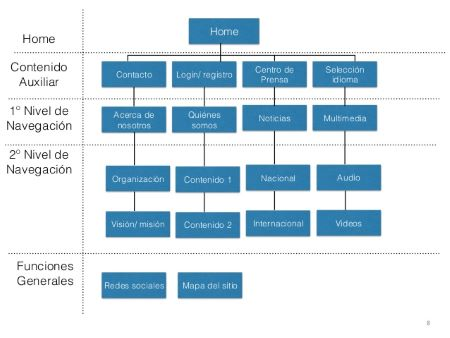
\includegraphics[width=.5\textwidth]{images/mapa}
		\caption{mapa}
		\label{fig:mapa}
	\end{center}
\end{figure}


%--------------------------------------
\section{IU1 Pantalla principal nutriologo}

\subsection{Objetivo}
	Permite al {\bf nutriologo} acceder a las principales funciones que tiene dentro del sistema

\subsection{Diseño}
	Esta pantalla \IUref{IU1}{Pantalla principal nutriologo} (ver figura~\ref{IU1}) aparece una vez que el usuario ha ingresado al sistema. 
 en la parte superior aparecen tres opciones de que acciones puede realizar el actor las cuales son {\bf añadir comida}, {\bf ver menú}, {\bf Cerrar Sesión}. 

 
%\IUfig[numero que modifica el tamaño de la imagen]{nombre de la imagen}{Id interfaz}{nombre interfaz.}
\IUfig[.7]{inicionutriologo}{IU1}{Pantalla principal nutriologo.}

\subsection{Salidas}

	Ninguna.

\subsection{Entradas}

        Ninguna.

\subsection{Comandos}
\begin{itemize}
	\item \IUbutton{Añadir comida}: muestra la \IUref{IU14}{Registrar comida}.
	\item \IUbutton{ver menú}: Muestra el menu de comidas de todo el mes
        \item \IUbutton{Cerrar sesión}Termina la sesion del usuario y lo saca del sistema
\end{itemize}

\subsection{Mensajes}
Ninguno.


\newpage
%--------------------------------------
\section{IU2 Pantalla principal medico}

\subsection{Objetivo}
	Permite al {\bf medico} acceder a las principales funciones que tiene dentro del sistema

\subsection{Diseño}
	Esta pantalla \IUref{IU2}{Pantalla principal medico} (ver figura~\ref{IU2}) aparece una vez que el usuario ha ingresado al sistema. 
 en la parte superior aparecen dos opciones de que acciones puede realizar el actor las cuales son {\bf Registrar incidente}, {\bf cerrar sesión}. 

 
%\IUfig[numero que modifica el tamaño de la imagen]{nombre de la imagen}{Id interfaz}{nombre interfaz.}
\IUfig[.7]{iniciomedico}{IU2}{Pantalla principal medico.}

\subsection{Salidas}

	Ninguna.

\subsection{Entradas}
        Ninguna.

\subsection{Comandos}
\begin{itemize}
	\item \IUbutton{Registrar incidente}: muestra la \IUref{IU20}{Incidencia médica}.
        \item \IUbutton{Cerrar sesión}Termina la sesion del usuario y lo saca del sistema
\end{itemize}

\subsection{Mensajes}

            Ninguno.

\newpage
%--------------------------------------
\section{IU3 Pantalla principal profesor}

\subsection{Objetivo}
	Permite al {\bf profesor} acceder a las principales funciones que tiene dentro del sistema

\subsection{Diseño}
	Esta pantalla \IUref{IU3}{Pantalla principal profesor} (ver figura~\ref{IU3}) aparece una vez que el usuario ha ingresado al sistema. 
 En la parte superior aparecen seis opciones de que acciones puede realizar el actor las cuales son: {\bf registrar ingesta}, {\bf registrar actividades}, {\bf Registrar tareas}, {\bf Registrar reporte}, {\bf Tomar asistencia}, {\bf Cerrar Sesión}. 

 
%\IUfig[numero que modifica el tamaño de la imagen]{nombre de la imagen}{Id interfaz}{nombre interfaz.}
\IUfig[.55]{iniciodocente}{IU3}{Pantalla principal profesor.}

\subsection{Salidas}

	Ninguna.

\subsection{Entradas}
        Ninguna.

\subsection{Comandos}
\begin{itemize}
	\item \IUbutton{Registrar ingesta}: muestra la \IUref{IU16}{Registrar ingesta}.
        \item \IUbutton{Registrar actividades}: muestra la \IUref{IU17}{Registrar actividades}.
        \item \IUbutton{Registrar tareas}: muestra la \IUref{IU18}{Registrar tareas}.
        \item \IUbutton{Registrar reporte}: muestra la \IUref{IU23}{Registrar reporte}.
        \item \IUbutton{Tomar asistencia}: muestra la \IUref{IU22}{Tomar asistencia}.
        \item \IUbutton{Cerrar sesión}Termina la sesion del usuario y lo saca del sistema
\end{itemize}

\subsection{Mensajes}

\begin{Citemize}
	\item Error al verificar los datos de acceso, vuelva a intentarlo.
\end{Citemize}


\newpage
%--------------------------------------
\newpage
\section{IU4 Pantalla principal Recursos Humanos}

\subsection{Objetivo}
	Permite a {\bf Recursos humanos} acceder a las principales funciones que tiene dentro del sistema

\subsection{Diseño}
	Esta pantalla \IUref{IU4}{Pantalla principal Recursos Humanos} (ver figura~\ref{IU4}) aparece una vez que el usuario ha ingresado al sistema. En la parte superior aparecen tres opciones de que acciones puede realizar el actor las cuales son {\bf Alimentacion},{\bf Docencia},{\bf Medicina}, {\bf Cerrar Sesión}.

 
%\IUfig[numero que modifica el tamaño de la imagen]{nombre de la imagen}{Id interfaz}{nombre interfaz.}
\IUfig[.9]{principalRecursosHumanos}{IU4}{Pantalla principal Recursos Humanos.}

\subsection{Salidas}

	Ninguna.

\subsection{Entradas}

Ninguna.

\subsection{Comandos}
\begin{itemize}
	\item \IUbutton{Alimentacion}: Muestra la \IUref{IU13}{registrar nutriologo}.
	\item \IUbutton{Docencia}: Muestra la \IUref{IU8}{registrar profesor}.
 	\item \IUbutton{Medicina}: Muestra la \IUref{IU19}{registrar medico}.
          \item \IUbutton{Cerrar sesión}Termina la sesion del usuario y lo saca del sistema
\end{itemize}

\subsection{Mensajes}

\begin{Citemize}
	\item Ninguno
\end{Citemize}


%--------------------------------------
\newpage
\section{IU5 Pantalla principal Capital humano}

\subsection{Objetivo}
	Permite a {\bf capital humano} acceder a las principales funciones que tiene dentro del sistema

\subsection{Diseño}
	La\IUref{IU5}{Pantalla principal de capital humano} (ver figura~\ref{IU5}) aparece una vez que el usuario ha ingresado al sistema. 
 en la parte superior aparecen tres opciones de que acciones puede realizar el actor las cuales son {\bf Tutor},{\bf Infantes},{\bf Salas},{\bf Cerrar Sesión}. 

 
%\IUfig[numero que modifica el tamaño de la imagen]{nombre de la imagen}{Id interfaz}{nombre interfaz.}
\IUfig[.9]{principalCapitalHumano}{IU5}{Pantalla principal capital humano.}

\subsection{Salidas}

	Ninguna.

\subsection{Entradas}
Ninguna.

\subsection{Comandos}
\begin{itemize}
	\item \IUbutton{Tutor}: Muestra la \IUref{IU9}{modificar tutores}.
	\item \IUbutton{Infantes}: Muestra la \IUref{IU10}{modificar  infantes}.
 	\item \IUbutton{Salas}: Muestra la \IUref{IU12}{modificar salas}.
        \item \IUbutton{Cerrar sesión}Termina la sesion del usuario y lo saca del sistema
\end{itemize}

\subsection{Mensajes}

\begin{Citemize}
	\item Ninguno.
\end{Citemize}


\newpage
%--------------------------------------
\section{IU6 Pantalla principal padre de familia}

\subsection{Objetivo}
	Permite al {\bf padre de familia} acceder a las principales funciones que tiene dentro del sistema

\subsection{Diseño}
	Esta pantalla \IUref{IU6}{Pantalla principal padre de familia} (ver figura~\ref{IU6}) aparece una vez que el usuario ha ingresado al sistema. 
 en la parte superior aparecen tres opciones de que acciones puede realizar el actor las cuales son {\bf Ver reportes},{\bf Contactar asesor},{\bf Cerrar Sesión}. 

 
%\IUfig[numero que modifica el tamaño de la imagen]{nombre de la imagen}{Id interfaz}{nombre interfaz.}
\IUfig[.9]{padreFamiliaIU}{IU6}{Pantalla principal padre de familia.}

\subsection{Salidas}

	Ninguna.

\subsection{Entradas}
nINGUNA

\subsection{Comandos}
\begin{itemize}
	\item \IUbutton{Ver reportes}: Muestra la \IUref{UI15}{Ver reportes de hijos}.
	\item \IUbutton{Contactar asesor}: Muestra el \IUref{UI15}{Formulario para contactarse con un asesor}.
          \item \IUbutton{Cerrar sesión}Termina la sesion del usuario y lo saca del sistema
\end{itemize}

\subsection{Mensajes}

\begin{Citemize}
	\item Ninguno
\end{Citemize}


%--------------------------------------
\newpage
\section{IU7 Pantalla principal director}

\subsection{Objetivo}
	Permite al {\bf director} acceder a las principales funciones que tiene dentro del sistema

\subsection{Diseño}
	Esta pantalla \IUref{IU7}{Pantalla principal director} (ver figura~\ref{IU7}) aparece una vez que el usuario ha ingresado al sistema. 
 en la parte superior aparecen tres opciones de que acciones puede realizar el actor las cuales son {\bf Agregar evento escolar},{\bf Cerrar Sesión}. 

 
%\IUfig[numero que modifica el tamaño de la imagen]{nombre de la imagen}{Id interfaz}{nombre interfaz.}
\IUfig[.9]{directorEventos}{IU7}{Pantalla principal del director.}

\subsection{Salidas}

	Ninguna.

\subsection{Entradas}
Ninguna

\subsection{Comandos}
\begin{itemize}
	\item \IUbutton{Agregar evento escolar}:Se muestra la \IUref{UI21}{Pantalla registrar evento escolar}.
          \item \IUbutton{Cerrar sesión}Termina la sesion del usuario y lo saca del sistema
\end{itemize}

\subsection{Mensajes}

\begin{Citemize}
	\item Nninguno.
\end{Citemize}


%--------------------------------------
\newpage
\section{IU8 Registrar profesor}

\subsection{Objetivo}
	Permite a {\bf Recursos Humanos} registrar un nuevo profesor.

\subsection{Diseño}
	Esta pantalla \IUref{IU8}{Registrar profesor} (ver figura~\ref{IU8}) aparece una vez que el usuario ha ingresado al aparte de Docente en la \IUref{IU4}{Pantalla principal Recursos Humanos}. 
    En la pantalla aparecen tres text area: {\bf Nombre},{\bf Dirección},{\bf Número de telefono}, y el botón{\bf Enviar}. 

 
%\IUfig[numero que modifica el tamaño de la imagen]{nombre de la imagen}{Id interfaz}{nombre interfaz.}
\IUfig[.9]{regdocente}{IU8}{Registrar profesor.}

\subsection{Salidas}

	Mensaje de registro éxitoso.

\subsection{Entradas}
Nombre, dirección y número de teléfono del profesor.

\subsection{Comandos}
\begin{itemize}
	\item \IUbutton{Enviar}: Envía el formulario para registar al profesor. 
\end{itemize}

\subsection{Mensajes}
\begin{Citemize}
	\item El profesor se registró con exito.
        \item Formato incorrecto, por favor vuelva a llenar el formulario.
        \item El profesor ya está registrado.
\end{Citemize}


\newpage
%--------------------------------------
\section{IU9 Registrar padre de familia}

\subsection{Objetivo}
	Permite a {\bf Capital Humano} registrar a un tutor o padre de familia.

\subsection{Diseño}
	Esta pantalla \IUref{IU9}{Registrar padre de familia} (ver figura~\ref{IU9}) aparece una vez que el usuario ha ingresado al apartado de Tutor en \IUref{IU5}{Pantalla principal de capital humano}. 
 En la pantalla aparecen tres text area: {\bf Nombre},{\bf Dirección},{\bf Número de telefono}, y el botón{\bf Enviar}. 
 
%\IUfig[numero que modifica el tamaño de la imagen]{nombre de la imagen}{Id interfaz}{nombre interfaz.}
\IUfig[.9]{regpadre}{IU9}{Registrar padre de familia.}

\subsection{Salidas}

	Ninguna.

\subsection{Entradas}
Número de Boleta y Contraseña del Estudiante.

\subsection{Comandos}
\begin{itemize}
	\item \IUbutton{Entrar}: Verifica que el Estudiante se encuentre registrado y la contraseña sea la correcta. Si la verificación es correcta, se muestra la \IUref{UI32}{Pantalla de Selección de Seminario}.
	\item \IUbutton{Ayuda}: Muestra la ayuda de esta pantalla \IUref{IU50}{Pantalla de Ayuda}.
\end{itemize}

\subsection{Mensajes}

\begin{Citemize}
	\item El tutor se registró con exito.
        \item Formato incorrecto, por favor vuelva a llenar el formulario.
        \item El tutor ya está registrado.
\end{Citemize}

\newpage
%--------------------------------------
\section{IU10 Registrar niño}

\subsection{Objetivo}
	Permite a {\bf Capital Humano} registrar a un nuevo niño en la guardería.

\subsection{Diseño}
	Esta pantalla \IUref{IU10}{Registrar niño} (ver figura~\ref{IU10}) aparece una vez que el usuario ha dado clic en la sección Infantes dentro de \IUref{IU5{Pantalla principal de capital humano}. 
    en la parte superior aparecen cinco cuadros de texto, las cuales son {\bf nombre},{\bf apellido paterno},{\bf apellido materno},{\bf fecha de nacimiento} y {\bf género}, además aparece el botón para enviar el formulario {\bf enviar}. 

 
%\IUfig[numero que modifica el tamaño de la imagen]{nombre de la imagen}{Id interfaz}{nombre interfaz.}
\IUfig[.9]{reginfante}{IU10}{Registrar niño.}

\subsection{Salidas}

	Mensaje de texto.

\subsection{Entradas}
Nombre completo, fecha de nacimiento y género del infante.

\subsection{Comandos}
\begin{itemize}
	\item \IUbutton{Enviar}: Envía el formulario para registar un nuevo infante
\end{itemize}

\subsection{Mensajes}

\begin{Citemize}
	\item Error con el formato de los datos, por favor vuelva a llenar el formulario.
        \item Infante registrado exitosamente.
        \item Error, el infante ya está registrado, por favor revise la información.
\end{Citemize}


\newpage
%--------------------------------------
\section{IU11 Enlazar infante}

\subsection{Objetivo}
	Permite a {\bf Capital HUmano} enlazar un tutor con un infante.

\subsection{Diseño}
	Esta pantalla \IUref{IU11}{Enlazar infante} (ver figura~\ref{IU11}) aparece una vez que el usuario ha ingresado al apartado de Infantes en \IUref{IU11}{Pantalla principal de capital humano}. 
    aparecen dos listas, una contiene a todos los tutores y la otra a los infantes con menos de dos tutores asignados, además el usuario puede seleccionar un padre y un niño para enlazar. Hay un botón para realizar esta acción: {\bf Enlazar}. 

 
%\IUfig[numero que modifica el tamaño de la imagen]{nombre de la imagen}{Id interfaz}{nombre interfaz.}
\IUfig[.9]{enlaceinfante}{IU11}{Enlazar infante.}

\subsection{Salidas}

	Mensaje de éxito.

\subsection{Entradas}
Tutor, Infante.

\subsection{Comandos}
\begin{itemize}
	\item \IUbutton{Enlazar}: Realiza una petición para enlazar el tutor seleccionado con el infante seleccionado.
\end{itemize}

\subsection{Mensajes}

\begin{Citemize}
	\item Éxito al enlzar.
\end{Citemize}


%--------------------------------------
\newpage
\section{IU12 Registrar sala}

\subsection{Objetivo}
	Permite a {\bf Capital Humano} registrar una sala donde se cuidaran a los infantes.

\subsection{Diseño}
	 Esta pantalla \IUref{IU12}{Registrar sala} (ver figura~\ref{IU12}) aparece cuando el            profesor selecciona el comando Salas en la \IUref{IU5}{Pantalla principal  profesor}. 
         en la parte superior aparecen tres opciones de que acciones puede realizar el actor las cuales son {\bf Tutor},{\bf Infantes},{\bf Salas},{\bf Cerrar Sesión}. 
         El contenido muestra dos inputs solicitando nombre de Sala y capacidad.
         en la parte de abajo tiene un boton que guarda las tareas en la bd
        
 
%\IUfig[numero que modifica el tamaño de la imagen]{nombre de la imagen}{Id interfaz}{nombre interfaz.}
\IUfig[.9]{regsala}{IU12}{Registrar sala.}

\subsection{Salidas}

	Ninguna.

\subsection{Entradas}
nombre de Sala y capacidad.

\subsection{Comandos}
\begin{itemize}
	\item \IUbutton{Tutor}: Muestra la \IUref{IU9}{modificar tutores}.
	\item \IUbutton{Infantes}: Muestra la \IUref{IU10}{modificar  infantes}.
 	\item \IUbutton{Salas}: Muestra la \IUref{IU12}{modificar salas}.
        \item \IUbutton{Cerrar sesión}Termina la sesion del usuario y lo saca del sistema.
        \item \IUbutton{Guardar} guarda la sala en la bd y muestra el MSGX
\end{itemize}

\subsection{Mensajes}

\begin{Citemize}
	\item Exito registrando la sala.
\end{Citemize}


%--------------------------------------
\section{IU13 Registrar nutriologo}

\subsection{Objetivo}
	Permite a {\bf recursos humanos} registrar a un nutriologo en el sistema

\subsection{Diseño}
	Esta pantalla \IUref{IU13}{Registrar nutriologo} (ver figura~\ref{IU13}) aparece una vez que el usuario ha ingresado al sistema y a seleccionado {\bf Alimentacion}
 en la parte superior aparecen una opcion la cual es {\bf regresar}, y en el contenido viene la lista de nutriologos actuales y la opcion de guardar un nuevo nutriologo o eliminar uno de la lista,{\bf Guardar},{\bf Eliminar}. 

 
%\IUfig[numero que modifica el tamaño de la imagen]{nombre de la imagen}{Id interfaz}{nombre interfaz.}
\IUfig[.9]{regnutriologo}{IU13}{Registrar nutriologo.}

\subsection{Salidas}

	Ninguna.

\subsection{Entradas}
Nombre, direccion, numero de telefono.

\subsection{Comandos}
\begin{itemize}
	\item \IUbutton{regresar}: permite al actor regresar a la \IUref{UI4}{Pantalla principal de recursos humanos}.
 	\item \IUbutton{Guardar}: permite a recursos humanos guardar un nuevo nutriologo en el sistema.
  	\item \IUbutton{Eliminar}: permite a recursos humanos eliminar a un nutriologo del sistema.
\end{itemize}

\subsection{Mensajes}

\begin{Citemize}
	\item Nuevo nutriologo registrado.
        \item Nutriologo eliminado.
\end{Citemize}


%--------------------------------------
\newpage
\section{IU14 Registrar comida}

\subsection{Objetivo}
	Permite al {\bf nutriologo} añadir una comida al menu del mes

\subsection{Diseño}
	Esta pantalla \IUref{IU14}{Registrar comida} (ver figura~\ref{IU14}) aparece cuando el nutriologo selecciona el comando registrar comida de la \IUref{IU1}{Pantalla principal nutriologo}. 
 En la parte superior aparecen tres opciones de que acciones puede realizar el actor las cuales son {\bf añadir comida}, {\bf ver menú}, {\bf Cerrar Sesión}. 
Tiene dos inputs para que el nutriologo los llena con el nombre de la comida y la fecha en la que se va a dar, ademas tiene tres radio boton donde se debe seleccionar uno para indicar el momento de la comida
 
%\IUfig[numero que modifica el tamaño de la imagen]{nombre de la imagen}{Id interfaz}{nombre interfaz.}
\IUfig[.9]{regcomida}{IU14}{Registrar comida.}

\subsection{Salidas}

	Ninguna.

\subsection{Entradas}
Nombre comida, KCalorias, Tiempo comida, Ingredientes

\subsection{Comandos}
\begin{itemize}
	\item \IUbutton{Añadir comida}: muestra la \IUref{IU14}{Registrar comida}.
	\item \IUbutton{ver menú}: Muestra el menu de comidas de todo el mes
        \item \IUbutton{Cerrar sesión}Termina la sesion del usuario y lo saca del sistema
        \item \IUbutton{Guardar} guarda la comida en la bd y muestra el MSGX
\end{itemize}

\subsection{Mensajes}

\begin{Citemize}
	\item MSGX Exito al guardar la comida
\end{Citemize}


%--------------------------------------
\section{IU15 Ver Reporte hijo}

\subsection{Objetivo}
	Permite al {\bf padre de familia} ver los reportes de su hijo creados por el sistema hasta el momento.

\subsection{Diseño}
	Esta pantalla \IUref{IU15}{Ver Reporte niño} (ver figura~\ref{IU15}) aparece una vez que el usuario ha ingresado al sistema y ha seleccionado el {\bf Ver reportes}. 
 en la parte superior aparecen una opcion de que acciones puede realizar el actor las cual es {\bf regresar} y en el contenido hay un calendario junto a un input de la fecha del reporte que requiera ver. 

 
%\IUfig[numero que modifica el tamaño de la imagen]{nombre de la imagen}{Id interfaz}{nombre interfaz.}
\IUfig[.9]{reporteinfante}{IU15}{Ver Reporte niño.}

\subsection{Salidas}

	Ninguna.

\subsection{Entradas}
Fecha.

\subsection{Comandos}
\begin{itemize}
	\item \IUbutton{Regresar}: Permite al padre de familia regresar a a la \IUref{UI6}{Pantalla principal padre de familia}.
\end{itemize}

\subsection{Mensajes}

\begin{Citemize}
	\item Ninguno.
\end{Citemize}


%--------------------------------------
\newpage
\section{IU16 Registrar ingesta}

\subsection{Objetivo}
	Permite al {\bf profesor} Registrar que tanto comieron los niños en una de las comidas del dia.

\subsection{Diseño}
	Esta pantalla \IUref{IU16}{Registrar ingesta} (ver figura~\ref{IU16}) aparece cuando el profesor selecciona el comando registrar ingesta en la \IUref{IU3}{Pantalla principal profesor}. 
 En la parte superior aparecen seis opciones de que acciones puede realizar el actor las cuales son: {\bf registrar ingesta}, {\bf registrar actividades}, {\bf Registrar tareas}, {\bf Registrar reporte}, {\bf Tomar asistencia}, {\bf Cerrar Sesión}. 
 El contenido muestra los nombres de los niños y tres opciones para mostrar cuanto comio
 en la parte de abajo tiene un boton que guarda las ingestas en la bd
 
%\IUfig[numero que modifica el tamaño de la imagen]{nombre de la imagen}{Id interfaz}{nombre interfaz.}
\IUfig[.7]{regingesta}{IU16}{Registrar ingesta.}

\subsection{Salidas}

	MSGX.

\subsection{Entradas}
TiempoComida

\subsection{Comandos}
\begin{itemize}
	\item \IUbutton{Registrar ingesta}: muestra la \IUref{IU16}{Registrar ingesta}.
        \item \IUbutton{Registrar actividades}: muestra la \IUref{IU17}{Registrar actividades}.
        \item \IUbutton{Registrar tareas}: muestra la \IUref{IU18}{Registrar tareas}.
        \item \IUbutton{Registrar reporte}: muestra la \IUref{IU23}{Registrar reporte}.
        \item \IUbutton{Tomar asistencia}: muestra la \IUref{IU22}{Tomar asistencia}.
        \item \IUbutton{Cerrar sesión}Termina la sesion del usuario y lo saca del sistema
        \item \IUbutton{Guardar} guarda las ingestas de los niños en la bd y muestra el MSGX
\end{itemize}


\subsection{Mensajes}

\begin{Citemize}
	\item MSGX Exito al guardar las ingestas
\end{Citemize}


%--------------------------------------
\newpage
\section{IU17 Registrar actividades}

\subsection{Objetivo}
	Permite al {\bf profesor} registrar las actividades que hicieron los infantes y que calificacion se les otorgo para que los padres puedan visualizarlo

\subsection{Diseño}
	 Esta pantalla \IUref{IU17}{Registrar actividades} (ver figura~\ref{IU17}) aparece cuando el            profesor selecciona el comando Registrar actividades en la \IUref{IU3}{Pantalla principal  profesor}. 
         En la parte superior aparecen seis opciones de que acciones puede realizar el actor las cuales son: {\bf registrar ingesta}, {\bf registrar actividades}, {\bf Registrar tareas}, {\bf Registrar reporte}, {\bf Tomar asistencia}, {\bf Cerrar Sesión}. 
         El contenido muestra tres inputs solicitando Número de Sala, detalles actividad, nombre actividad y ponderacion
         en la parte de abajo tiene un boton que guarda las actividades en la bd
         
%\IUfig[numero que modifica el tamaño de la imagen]{nombre de la imagen}{Id interfaz}{nombre interfaz.}
\IUfig[.9]{regactividades}{IU17}{Registrar actividades.}

\subsection{Salidas}

	Ninguna.

\subsection{Entradas}
Número de Sala, nombre actividad, detalles actividad, puntos.

\subsection{Comandos}
\begin{itemize}
	\item \IUbutton{Registrar ingesta}: muestra la \IUref{IU16}{Registrar ingesta}.
        \item \IUbutton{Registrar actividades}: muestra la \IUref{IU17}{Registrar actividades}.
        \item \IUbutton{Registrar tareas}: muestra la \IUref{IU18}{Registrar tareas}.
        \item \IUbutton{Registrar reporte}: muestra la \IUref{IU23}{Registrar reporte}.
        \item \IUbutton{Tomar asistencia}: muestra la \IUref{IU22}{Tomar asistencia}.
        \item \IUbutton{Cerrar sesión}Termina la sesion del usuario y lo saca del sistema
        \item \IUbutton{Guardar} guarda la actividad de los niños en la bd y muestra el MSGX
\end{itemize}

\subsection{Mensajes}

\begin{Citemize}
	\item Exito al guardar la actividad.
\end{Citemize}


%--------------------------------------
\newpage
\section{IU18 Registrar tareas}

\subsection{Objetivo}
	Permite al {\bf profesor} registrar las tareas que deben hacer los infantes en sus casas, para que los padres de familia esten enterados de estas.

\subsection{Diseño}
	 Esta pantalla \IUref{IU18}{Registrar tareas} (ver figura~\ref{IU18}) aparece cuando el            profesor selecciona el comando Registrar tareas en la \IUref{IU3}{Pantalla principal  profesor}. 
         En la parte superior aparecen seis opciones de que acciones puede realizar el actor las cuales son: {\bf registrar ingesta}, {\bf registrar actividades}, {\bf Registrar tareas}, {\bf Registrar reporte}, {\bf Tomar asistencia}, {\bf Cerrar Sesión}. 
         El contenido muestra tres inputs solicitando Número de Sala, detalles actividad, nombre actividad, ponderacion y fecha de entrega.
         en la parte de abajo tiene un boton que guarda las tareas en la bd
        
 
%\IUfig[numero que modifica el tamaño de la imagen]{nombre de la imagen}{Id interfaz}{nombre interfaz.}
\IUfig[.9]{regtareas}{IU18}{Registrar tareas.}

\subsection{Salidas}

	Ninguna.

\subsection{Entradas}
Número de Sala, detalles actividad, nombre actividad, ponderacion y fecha de entrega.

\subsection{Comandos}
\begin{itemize}
	\item \IUbutton{Registrar ingesta}: muestra la \IUref{IU16}{Registrar ingesta}.
        \item \IUbutton{Registrar actividades}: muestra la \IUref{IU17}{Registrar actividades}.
        \item \IUbutton{Registrar tareas}: muestra la \IUref{IU18}{Registrar tareas}.
        \item \IUbutton{Registrar reporte}: muestra la \IUref{IU23}{Registrar reporte}.
        \item \IUbutton{Tomar asistencia}: muestra la \IUref{IU22}{Tomar asistencia}.
        \item \IUbutton{Cerrar sesión}Termina la sesion del usuario y lo saca del sistema.
        \item \IUbutton{Guardar} guarda la tarea de los niños en la bd y muestra el MSGX.
\end{itemize}

\subsection{Mensajes}

\begin{Citemize}
	\item Exito al guardar la tarea.
\end{Citemize}


%--------------------------------------
\newpage
\section{IU19 Registrar medico}

\subsection{Objetivo}
	Permite a {\bf Recursos Humanos} registrar las actividades que hicieron los infantes y que calificacion se les otorgo para que los padres puedan visualizarlo

\subsection{Diseño}
	 Esta pantalla \IUref{IU19}{Registrar médico} (ver figura~\ref{IU19}) aparece cuando el            profesor selecciona el comando medicina en la \IUref{IU4}{Pantalla principal  recursos humanos}. 
         En la parte superior aparecen cuatro opciones de que acciones puede realizar el actor las cuales son: {\bf Alimentacion}, {\bf Docencia}, {\bf Medicina}, {\bf Cerrar sesión}. 
         El contenido muestra tres inputs solicitando Número de Sala, detalles actividad, nombre actividad y ponderacion
         en la parte de abajo tiene un boton que guarda al médico en la bd
 
%\IUfig[numero que modifica el tamaño de la imagen]{nombre de la imagen}{Id interfaz}{nombre interfaz.}
\IUfig[.9]{regmedico}{IU19}{Registrar medico.}

\subsection{Salidas}

	Ninguna.

\subsection{Entradas}
Nombre, licencia medica, fecha nacimiento, salario, curp, telefono, direccion.

\subsection{Comandos}
\begin{itemize}
	\item \IUbutton{Alimentacion}: Muestra la \IUref{IU13}{registrar nutriologo}.
	\item \IUbutton{Docencia}: Muestra la \IUref{IU8}{registrar profesor}.
 	\item \IUbutton{Medicina}: Muestra la \IUref{IU19}{registrar medico}.
        \item \IUbutton{Guardar}: Registra al médico en la BD y muestra el MSGX
        \item \IUbutton{Cerrar sesión}: Termina la sesion del usuario y lo saca del sistema
\end{itemize}

\subsection{Mensajes}

\begin{Citemize}
	\item Exito registrando al médico.
\end{Citemize}


%--------------------------------------
\newpage
\section{IU20 Registrar incidencia medica}

\subsection{Objetivo}
	Permite al {\bf médico} Registrar el estado de un infante cuando ocurre un incidente.

\subsection{Diseño}
	Esta pantalla \IUref{IU20}{Registrar incidencia medica} (ver figura~\ref{IU20}) aparece cuando el medico selecciona el comando registrar incidencia de la \IUref{IU2}{pantalla principal medico}. 
En la parte superior aparecen dos opciones de que acciones puede realizar el actor las cuales son {\bf Registrar incidente}, {\bf cerrar sesión}.
Se pueden observar dos input text que solicitan la boleta del infante y los detalles del incidente, asi como una seccion con rario button para que el medico seleccione una opcion de acuerdo con el status del infante
 
%\IUfig[numero que modifica el tamaño de la imagen]{nombre de la imagen}{Id interfaz}{nombre interfaz.}
\IUfig[.9]{regincidenciamedica}{IU20}{Registrar incidencia medica.}

\subsection{Salidas}

	Ninguna.

\subsection{Entradas}
Número de Boleta EstadoInfante y detalles.

\subsection{Comandos}
\begin{itemize}
	\item \IUbutton{Registrar incidente}: muestra la \IUref{IU20}{Incidencia médica}.
        \item \IUbutton{Cerrar sesión}Termina la sesion del usuario y lo saca del sistema
        \item \IUbutton{Guardar} guarda la incidencia del infante en la bd y muestra el MSGX
\end{itemize}

\subsection{Mensajes}

\begin{Citemize}
	\item Exito al guardar el incidente del infante.
\end{Citemize}


%--------------------------------------
\section{IU21 Registrar evento escolar}

\subsection{Objetivo}
	Permite al {\bf director} registrar un evento escolar

\subsection{Diseño}
	Esta pantalla \IUref{IU21}{Registrar evento escolar} (ver figura~\ref{IU21}) aparece una vez que el usuario ha ingresado al sistema y ha seleccionado agregar evento escolar,
 en la parte superior aparecen tres opciones de que acciones puede realizar el actor las cuales son {\bf Regresar} y en la parte de la pantalla un formulario con los datos para ingresar un nuevo evento escolar y la opcion de {\bf Guardar} o {\bf Eliminar} del calendario. 

 
%\IUfig[numero que modifica el tamaño de la imagen]{nombre de la imagen}{Id interfaz}{nombre interfaz.}
\IUfig[.9]{regeventoescolar}{IU21}{Registrar evento escolar.}

\subsection{Salidas}

	Ninguna.

\subsection{Entradas}
fecha del evento, nombre del evento, hora de inicio y fin del evento.

\subsection{Comandos}
\begin{itemize}
	\item \IUbutton{Regresar}: regresa a la \IUref{UI7}{Pantalla del director}.
	\item \IUbutton{Guardar}: Guarda el evento creado.
           \item \IUbutton{Elimnar}: Elimina el evento seleccionado.
\end{itemize}

\subsection{Mensajes}

\begin{Citemize}
	\item Error al verificar los datos de acceso, vuelva a intentarlo.
\end{Citemize}


%--------------------------------------
\newpage
\section{IU22 tomar asistencia}

\subsection{Objetivo}
	Permite al {\bf profesor} tomar la asistencia de los niños para saber que niños se encuentran en la guarderia el dia de hoy

\subsection{Diseño}
	   Esta pantalla \IUref{IU22}{Tomar asistencia} (ver figura~\ref{IU22}) aparece cuando el            profesor selecciona el comando Tomar asistencia en la \IUref{IU3}{Pantalla principal  profesor}. 
         En la parte superior aparecen seis opciones de que acciones puede realizar el actor las cuales son: {\bf registrar ingesta}, {\bf registrar actividades}, {\bf Registrar tareas}, {\bf Registrar reporte}, {\bf Tomar asistencia}, {\bf Cerrar Sesión}. 
         El contenido muestra los nombres de los niños y dos opciones para registrar si asistio o no
         en la parte de abajo tiene un boton que guarda las ingestas en la bd
         
 
%\IUfig[numero que modifica el tamaño de la imagen]{nombre de la imagen}{Id interfaz}{nombre interfaz.}
\IUfig[.8]{tomarasistencia}{IU22}{Tomar asistencia.}

\subsection{Salidas}

	Ninguna.

\subsection{Entradas}
        Ninguna.

\subsection{Comandos}
\begin{itemize}
	\item \IUbutton{Registrar ingesta}: muestra la \IUref{IU16}{Registrar ingesta}.
        \item \IUbutton{Registrar actividades}: muestra la \IUref{IU17}{Registrar actividades}.
        \item \IUbutton{Registrar tareas}: muestra la \IUref{IU18}{Registrar tareas}.
        \item \IUbutton{Registrar reporte}: muestra la \IUref{IU23}{Registrar reporte}.
        \item \IUbutton{Tomar asistencia}: muestra la \IUref{IU22}{Tomar asistencia}.
        \item \IUbutton{Cerrar sesión}Termina la sesion del usuario y lo saca del sistema
        \item \IUbutton{Guardar} guarda la asistencia de los niños en la bd y muestra el MSGX
\end{itemize}


\subsection{Mensajes}

\begin{Citemize}
	\item Exito al guardar la asistencia
\end{Citemize}


%--------------------------------------
\section{IU23 Registrar reporte}

\subsection{Objetivo}
	Generar los reportes y guardarlos con su respectivo infante.

\subsection{Diseño}
	 Esta pantalla \IUref{IU23}{Registrar reporte} (ver figura~\ref{IU23}) aparece cuando el            profesor selecciona el comando Registrar reporte en la \IUref{IU3}{Pantalla principal  profesor}. 
         En la parte superior aparecen seis opciones de que acciones puede realizar el actor las cuales son: {\bf registrar ingesta}, {\bf registrar actividades}, {\bf Registrar tareas}, {\bf Registrar reporte}, {\bf Tomar asistencia}, {\bf Cerrar Sesión}. 
         El contenido muestra cuatro inputs solicitando informacion adicional, numero de cambios de ropa, numero de evacuaciones y la opcion de generar el reporte para los infantes que ya tienen echo su reporte, con el boton de registrar.
         
        
\IUfig[.8]{regreporte}{IU23}{Registrar reporte.}

\subsection{Salidas}

	Ninguna.

\subsection{Entradas}
Evacuaciones, cambios de ropa, informacion adicional, registrar reporte, 

\subsection{Comandos}
\begin{itemize}
	\item \IUbutton{Registrar ingesta}: muestra la \IUref{IU16}{Registrar ingesta}.
        \item \IUbutton{Registrar actividades}: muestra la \IUref{IU17}{Registrar actividades}.
        \item \IUbutton{Registrar tareas}: muestra la \IUref{IU18}{Registrar tareas}.
        \item \IUbutton{Registrar reporte}: muestra la \IUref{IU23}{Registrar reporte}.
        \item \IUbutton{Tomar asistencia}: muestra la \IUref{IU22}{Tomar asistencia}.
        \item \IUbutton{Cerrar sesión}Termina la sesion del usuario y lo saca del sistema.
        \item \IUbutton{Registrar} registra el reporte creado anteriormente con los infantes seleccionados.
\end{itemize}

\subsection{Mensajes}

\begin{Citemize}
	\item Exito al registrar los reportes.
\end{Citemize}




%=========================================================
%=========================================================
\chapter{Modelo de manejo de la información.}	

El modelo de manejo de la información es un aspecto crucial en el diseño del sistema de la guardería "Guardería Burbujas". Este modelo se enfoca en cómo se gestiona y accede a la información dentro del sistema, especialmente a través de consultas a la base de datos. El manejo efectivo de la información es fundamental para garantizar un funcionamiento óptimo del sistema y satisfacer las necesidades de los usuarios.

En el contexto de la guardería "Guardería Burbujas", el modelo de manejo de la información se centra en cómo se almacenan y recuperan los datos relacionados con los niños, los padres, las actividades, los horarios y otros aspectos relevantes para la gestión de la guardería. Una base de datos es utilizada para almacenar esta información de manera estructurada y eficiente.
\\

El modelo de manejo de la información se basa en el uso de consultas para acceder y manipular los datos almacenados en la base de datos. Las consultas son instrucciones o comandos que se envían a la base de datos para recuperar información específica de acuerdo a ciertos criterios o realizar operaciones de actualización en los datos.

En el sistema de la guardería "Guardería Burbujas", se utilizan consultas para diversas funcionalidades, como:

\begin{itemize}
\item Obtener la lista de niños y sus datos personales.
\item Buscar los horarios de las actividades para un día determinado.
\item Registrar la asistencia de los niños a las actividades.
\end{itemize}

Para realizar estas consultas, se utilizan lenguajes de consultas se usan funciones de \textbf{Mongoose} para la base de datos MongoDB que pueden ser usadas tambien en \textbf{CosmosDB}

El diseño adecuado del modelo de manejo de la información es esencial para garantizar un acceso eficiente y preciso a los datos en el sistema de la guardería "Guardería Burbujas". Se deben considerar aspectos como la estructura de la base de datos, la indexación de los datos, la optimización de consultas y la seguridad de la información.
\\

En este capítulo, se presentarán las técnicas y consideraciones clave en el diseño del modelo de manejo de la información en el sistema de la guardería "Guardería Burbujas". Se analizará la estructura de la base de datos que son collecciones en base a las entidades previamente echas.


\begin{figure}[htbp]
\centering
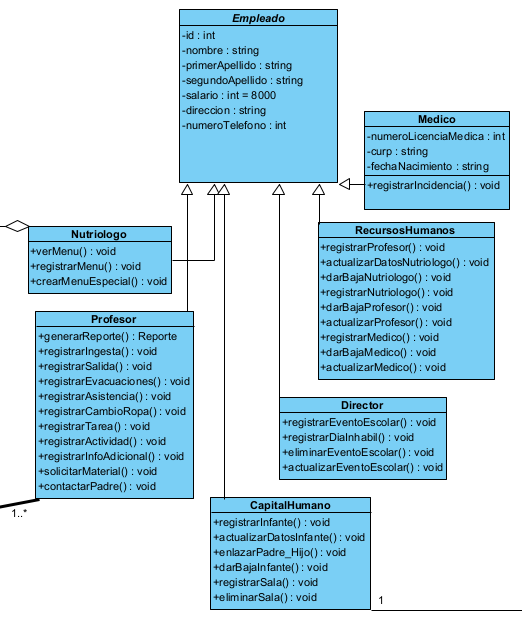
\includegraphics[width=0.4\textwidth]{images/arqui/comEmpleados.png}
\caption{Diagrama de la coleccion de las entidades de los empleados}
\label{fig:colecEmp}
\end{figure}

\begin{figure}[htbp]
\centering
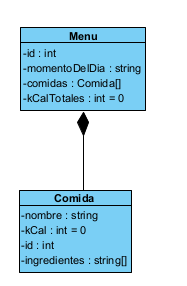
\includegraphics[width=0.4\textwidth]{images/arqui/colmenuComida.png}
\caption{Diagrama de la coleccion del menu y las comidas}
\label{fig:colecMenucCOM}
\end{figure}

\begin{figure}[htbp]
\centering
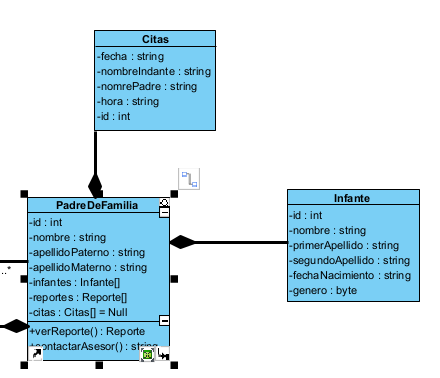
\includegraphics[width=0.4\textwidth]{images/arqui/colPadreFamilia.png}
\caption{Diagrama de la coleccion deL padre de familia}
\label{fig:colecPadre}
\end{figure}

\begin{figure}[htbp]
\centering
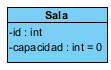
\includegraphics[width=0.4\textwidth]{images/arqui/sala.png}
\caption{Diagrama de la coleccion de una sala}
\label{fig:colecSala}
\end{figure}

\begin{figure}[htbp]
\centering
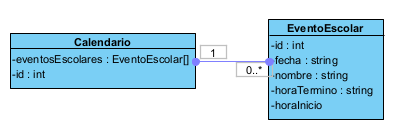
\includegraphics[width=0.4\textwidth]{images/arqui/colCaEv.png}
\caption{Diagrama de la coleccion deL calendario con Eventos Escolares}
\label{fig:colecEventCald}
\end{figure}
\clearpage

%======================================================================
\section{Consultas para el Caso de Uso CU1}

\begin{itemize}
    \item \textbf{Consulta001} usada para registrar un profesor
\end{itemize}

\begin{verbatim}
const nuevoProfesor = new Profesor({
  nombre: <nombreProfesor>,
  direccion: <direccionProfesor>,
  numeroTelefono: <numeroTelefonoProfesor>
});
    
nuevoProfesor.save();
\end{verbatim}


%======================================================================
\section{Consultas para el Caso de Uso CU2}

\begin{itemize}
    \item \textbf{Consulta002} usada para registrar un padre de familia.
\end{itemize}

\begin{verbatim}
const nuevoPadre = new PadredeFamilia({
  nombre: <nombrePadre>,
  direccion: <direccionPadre>,
  numeroTelefono: <numeroTelefonoPadre>
});
    
nuevoPadre.save();
\end{verbatim}


%======================================================================
\section{Consultas para el Caso de Uso CU3}

\begin{itemize}
    \item \textbf{Consulta003} usada para registrar un infante en el sistema.
\end{itemize}

\begin{verbatim}
const nuevoInfante = new Infante({
  nombre: <nombreInfante>,
  direccion: <direccionInfante>,
  fechaNacimiento: <fechaNacimientoInfante>
});
    
nuevoPadre.save();
\end{verbatim}


%======================================================================
\section{Consultas para el Caso de Uso CU4}

\begin{itemize}
    \item \textbf{Consulta004} usada para enlazar un padre con su hijo en la guarderia
\end{itemize}

\begin{verbatim}
Padre.findOne({ id: <idPadre> }).exec((error, padre) => {
  if (error) {
    console.log(error);
  } else {
    padre.infantes.push(<infante>);
    padre.save();
  }
});
\end{verbatim}


%======================================================================
\section{Consultas para el Caso de Uso CU5}

\begin{itemize}
    \item \textbf{Consulta005} llenado de datos de una sala para ser registrada
\end{itemize}

\begin{verbatim}
const nuevaSala = new Sala({
  capacidad: <numeroCapacidad>,
});
    
nuevaSala.save();
\end{verbatim}


%======================================================================
\section{Consultas para el Caso de Uso CU6}

\begin{itemize}
    \item \textbf{Consulta006} registro de un nuevo nutriologo
\end{itemize}

\begin{verbatim}
const nuevoNutriologo = new Nutriologo({
  nombre: <nombreNutriologo>,
  direccion: <direccionNutriologo>,
  numeroTelefono: <numeroTelefonoNutriologo>
});
    
nuevoNutriologo.save();

\end{verbatim}

\begin{itemize}
    \item \textbf{Consulta026} Eliminar nutriologo
\end{itemize}

\begin{verbatim}


nutriologo = Nutriologo.findOne({nombre: <nombreNutriologo> });

Nutriologo.deleteOne({id: <nutriolog.id> });
\end{verbatim}


%======================================================================
\section{Consultas para el Caso de Uso CU7}

\begin{itemize}
    \item \textbf{Consulta007} registro de comidas para el menu
\end{itemize}

\begin{verbatim}
const nuevoMenu = new Menu({
  momentoDelDia: <momentoDelDiaMenu>,

});
nuevoMenu.save();


const nuevaComida = new Comida({
  nombre: <nombreComida>,
  kCal: <numeroKCalorias>,
  ingredientes: <ingredientesComida>
});
    
nuevaComida.save();
nuevoMenu.comidas.push(nuevaComida);
nuevoMenu.save();

\end{verbatim}


%======================================================================
\section{Consultas para el Caso de Uso CU8}

\begin{itemize}
    \item \textbf{Consulta008} generar Cita con tutor
\end{itemize}

\begin{verbatim}
const nuevaCita = new Cita({
  nomreInfante: <nombreInfante>,
  nomrePadre: <nombrePadre>,
  fecha: <fechaCita>,
  hora: <horaCita>,
});
nuevaCita.save();

padre.citas.push(nuevaCita);
padre.save();

\end{verbatim}

%======================================================================
\section{Consultas para el Caso de Uso CU9}

\begin{itemize}
    \item \textbf{Consulta009} registrar ingesta en el reporte
\end{itemize}

\begin{verbatim}
reporteInfanteA.ingesta.push(<Ingesta>);
reporteInfanteA.save();
\end{verbatim}


%======================================================================
\section{Consultas para el Caso de Uso CU11}

\begin{itemize}
    \item \textbf{Consulta011} registrar actividades realizadas en el reporte
\end{itemize}

\begin{verbatim}
reporteInfanteA.actividades.push(<ActividadRealizada>);
reporteInfanteA.save();
\end{verbatim}

%======================================================================
\section{Consultas para el Caso de Uso CU12}

\begin{itemize}
    \item \textbf{Consulta012} registrar tareas en el reporte
\end{itemize}

\begin{verbatim}
reporteInfanteA.tareas.push(<tarea>);
reporteInfanteA.save();
\end{verbatim}

%======================================================================
\section{Consultas para el Caso de Uso CU14}

\begin{itemize}
    \item \textbf{Consulta014} registra medico en el sistema
\end{itemize}

\begin{verbatim}

const nuevoMedico = new Medico({
  nombre: <nombreMedico>,
  direccion: <direccionMedico>,
  numeroTelefono: <numeroTelefonoMedico>,
  numeroLicenciaMedica: <numeroLicenciaMedico>,
  curp: <curpMedico>,
  fechaNacimiento: <fechaNacimientoMedico>
});
    
nuevoMedico.save();

\end{verbatim}



\begin{itemize}
    \item \textbf{Consulta025} eliminar medico en el sistema
\end{itemize}

\begin{verbatim}
medico = Medico.findOne({nombre: <nombreMedico> });

Medico.deleteOne({id: <medico.id> });



\end{verbatim}

%======================================================================
\section{Consultas para el Caso de Uso CU15}

\begin{itemize}
    \item \textbf{Consulta015} registrar incidencia medica en el reporte
\end{itemize}

\begin{verbatim}
incidencia = ["Incidencia medica:", <Detalles>, <Estado infante>]
reporteInfanteA.informacionAdicional.push(<incidencia>);
\end{verbatim}

%======================================================================
\section{Consultas para el Caso de Uso CU17}

\begin{itemize}
    \item \textbf{Consulta017} registrar evento escolar
\end{itemize}

\begin{verbatim}
const nuevoEvento = new Evento({
  nombre: <nombreEvento>,
  fecha: <fechaEvento>,
  horaInicio: <horaInicioEvento>,
  horaTermino: <horaTerminoEvento>
});
nuevoEvento.save();
calendario.eventosEscolares.push(nuevoEvento);
calendario.save();
\end{verbatim}

\begin{itemize}
    \item \textbf{Consulta024} Eliminar evento escolar
\end{itemize}

\begin{verbatim}
calendario.updateOne(
  { $pull: { eventosEscolares: { id: <nuevoEvento.id> } } } 
);
\end{verbatim}


%======================================================================
\section{Consultas para el Caso de Uso CU19}

\begin{itemize}
    \item \textbf{Consulta019} Para que el profesor registre asistencia de los infantes
\end{itemize}

\begin{verbatim}
reporteInfanteA.asistencia = True;
reporteInfanteA.save();
\end{verbatim}

%======================================================================
\section{Consultas para el Caso de Uso CU22}

\begin{itemize}
    \item \textbf{Consulta022} El profesor registra el reporte del infante
\end{itemize}

\begin{verbatim}
const nuevoReporte = new Reporte({
  asistencia: <asistenciaInfante>,
  evacuaciones: <evacuacionesInfate>,
  ingesta: <ingestaInfante>,
  cambioRopa: <cambioRopaInfante>,
  actividades: <actividadesInfante>,
  tareas: <tareasInfante>,
  fecha: Date.now
});
nuevoReporte.save();

padre.reportes.push(nuevoReporte)
\end{verbatim}


%=========================================================
% ========================================================
%==========================================================
\part{Diseño}

%=========================================================
%=========================================================
\chapter{Introducción}

	Este documento contiene la Especificacion del diseño sobre el proyecto ``{\em "Guarderıa Burbujas”}'' correspondiente al trabajo realizado en el 2023/1 para la materia de Análisis y diseño de sistemas en el grupo 4BM1 por el equipo {\em Los bubulusuaves}.

%---------------------------------------------------------
\section{Presentación}

Este documento contiene la especificación de los requerimientos del usuario y del sistema para el diseño y desarrollo del sistema de la guardería. Su objetivo principal es establecer una base clara y precisa de los elementos necesarios para construir un sistema que cumpla con las necesidades y expectativas de los usuarios finales, así como con los requisitos técnicos y funcionales.

\begin{itemize}
\item Los requerimientos del usuario se centran en comprender y documentar las necesidades específicas de los usuarios finales de la guardería. Esto implica identificar las funcionalidades y características que el sistema debe ofrecer para satisfacer estas necesidades, como la gestión de la información de los infantes, el control de acceso de los padres, la generación de reportes, entre otros.


\item Los requerimientos del sistema se enfocan en definir las características técnicas, funcionales y de rendimiento que el sistema de la guardería debe cumplir. Esto incluye aspectos como la arquitectura del sistema, las interfaces de usuario, la seguridad de los datos, la escalabilidad para manejar un crecimiento futuro, la integración con otros sistemas, entre otros aspectos técnicos relevantes.
\end{itemize}

Al establecer estos requerimientos, se busca garantizar la calidad y el éxito del sistema de la guardería, asegurando su alineación con los objetivos del proyecto y la satisfacción de los usuarios finales. Además, estos requerimientos servirán como referencia durante todo el ciclo de vida del proyecto, facilitando la toma de decisiones, el seguimiento del progreso y la comunicación efectiva entre todos los involucrados en el desarrollo del sistema.

En resumen, este documento de especificación de requerimientos tiene como objetivo principal sentar las bases para el diseño y desarrollo exitoso del sistema de la guardería, asegurando una comprensión compartida de las necesidades y expectativas, tanto de los usuarios finales como del sistema en sí mismo
	
%---------------------------------------------------------
\section{Nomenclatura.}

	La información del presente documento se encuentra estructurada mediante diagramas, tablas y secciones con nomenclaturas y estándares específicos. Este capítulo tiene como finalidad indicar la forma en que se deben leer estos elementos para un mejor entendimiento.

%---------------------------------------------------------

%---------------------------------------------------------
\subsection{Diseño Arquitectónico}
El diseño arquitectónico se enfoca en definir la estructura general del sistema, incluyendo la distribución de los componentes, los patrones de interacción y las decisiones clave relacionadas con la arquitectura del sistema. Este diseño proporciona una visión de alto nivel de cómo se organiza y se relaciona cada componente del sistema, y cómo se cumplen los requerimientos funcionales y no funcionales. Al crear un diseño arquitectónico sólido, se busca maximizar la escalabilidad, la modularidad, la seguridad y el rendimiento del sistema.
%----------------------------------------------------------------

\subsection{ Modelado Estatico.}
Se enfoca en representar y describir la estructura y relaciones estáticas del sistema en desarrollo. Este modelado permite comprender los elementos del sistema y cómo se relacionan entre sí, sin tener en cuenta su comportamiento dinámico. El modelado estático incluye diagramas de clases, diagramas de componentes, diagramas de despliegue y otras técnicas que ayudan a visualizar y analizar la arquitectura del sistema desde una perspectiva estática mediante modulos.


El diseño de módulos se centra en la división del sistema en componentes más pequeños y cohesivos, llamados módulos. Estos módulos representan unidades funcionales independientes que pueden ser desarrolladas, probadas y mantenidas de manera individual. El diseño de módulos busca maximizar la cohesión dentro de cada módulo, lo que significa que las funcionalidades relacionadas se agrupan juntas, y minimizar la dependencia entre módulos, lo que permite cambios más fáciles y flexibilidad en el desarrollo del sistema.


Los diagramas de casos de uso son una herramienta usada para representar las transacciones entre un actor y el sistema, las cuales siempre tendrán un valor agregado o un propósito para que el actor las realice. En estos diagramas se podrán observar los siguientes elementos:

\begin{itemize}
    \item Representa al sistema mediante un óvalo.
    \begin{minipage}{0.2\textwidth}
        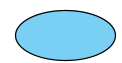
\includegraphics[width=0.1\linewidth]{images/ovalo.png}
    \end{minipage}
    \item Representa al actor que va a interactuar con el sistema.
    \begin{minipage}{0.2\textwidth}
        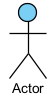
\includegraphics[width=0.1\linewidth]{images/actor.png}
    \end{minipage}
    \item Relación \texttt{<<extends>>}. Indica que un caso de uso puede ejecutarse a partir de otro.
    \item Relación \texttt{<<include>>}. Indica que un caso de uso debe ejecutarse a partir de otro.
\end{itemize}

La conexión entre un actor y un caso de uso se realiza mediante una línea como se muestra en la Figura 1.1.

\begin{figure}[htbp]
    \centering
    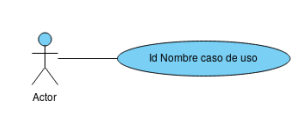
\includegraphics[width=0.4\textwidth]{images/interaccion.png}
    \caption{Interacción del actor con el caso de uso}
    \label{fig:interaccion-actor-caso-uso}
\end{figure}

Los casos de uso se encontrarán dentro de paquetes (representados por carpetas) indicando así que pertenecen a un mismo módulo, como se muestra en la Figura 1.2.

\begin{figure}[htbp]
    \centering
    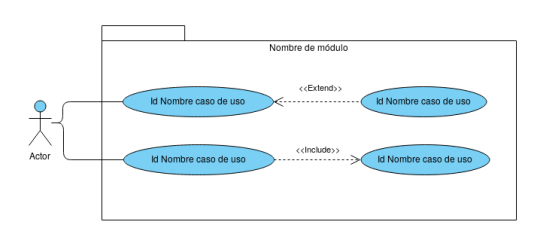
\includegraphics[width=0.6\textwidth]{images/interaccion2.png}
    \caption{Un Actor con varios casos de uso dentro de un módulo}
    \label{fig:actor-varios-casos-uso-modulo}
\end{figure}


%---------------------------------------------------------
\subsection{ Modelado Dinámico.}

Se centra en capturar y representar el comportamiento y las interacciones del sistema a lo largo del tiempo. Se utiliza para describir cómo los diferentes componentes del sistema interactúan entre sí y cómo se llevan a cabo las acciones y procesos. El modelado dinámico se realiza mediante diagramas de secuencia, diagramas de actividad, diagramas de estado y otras técnicas que permiten visualizar y analizar el flujo de eventos y el comportamiento dinámico del sistema.




%---------------------------------------------------------
\subsection{Modelos de Manejo de la Información}
Los modelos de manejo de la información se refieren a la representación y estructuración de los datos que serán almacenados y manipulados por el sistema. Estos modelos describen las entidades, atributos y relaciones entre los datos, y pueden incluir diagramas de entidad-relación, diagramas de clase y otros diagramas que ayudan a visualizar y comprender la estructura de los datos. El diseño de los modelos de manejo de la información busca garantizar la integridad, consistencia y eficiencia en la gestión de los datos, así como la adaptación a las necesidades específicas del sistema de la guardería.

Al abordar estos temas en el diseño del sistema de la guardería, se busca establecer una arquitectura sólida, modular y eficiente, así como una gestión efectiva de la información. Estos elementos son fundamentales para garantizar el rendimiento, la escalabilidad y la usabilidad del sistema, y para satisfacer las necesidades y expectativas de los usuarios finales.

%=========================================================
%=========================================================
\chapter{Diseño Arquitectónico}
\label{cap:reqUsr}

	Es una etapa clave en el desarrollo del sistema, donde se establecen las bases para su construcción y funcionamiento. En esta sección, se abordarán diversos aspectos relacionados con la arquitectura del sistema, como las propiedades del software, la plataforma utilizada, el costo y la arquitectura misma.

En cuanto a las propiedades del software, se considerarán aspectos como la modularidad, la escalabilidad, la flexibilidad y la fiabilidad. Estas propiedades son fundamentales para garantizar que el sistema pueda adaptarse a cambios futuros, crecer en función de las necesidades del usuario y mantener un rendimiento óptimo en diferentes situaciones.\\

La elección de la plataforma del sistema es otro aspecto importante a considerar. Esto incluye seleccionar el entorno de desarrollo, el lenguaje de programación, las herramientas y los frameworks que serán utilizados para implementar el sistema. La elección adecuada de la plataforma puede tener un impacto significativo en la eficiencia del desarrollo y en el rendimiento del sistema final.

El costo es otro factor crítico a tener en cuenta durante el diseño arquitectónico. Se deben considerar los recursos financieros disponibles, así como los costos asociados con la adquisición de hardware, licencias de software, mantenimiento y capacitación. El diseño arquitectónico debe buscar un equilibrio entre las funcionalidades y características deseadas y los recursos disponibles.\\

En cuanto a la arquitectura del sistema, se definirán los componentes principales, sus interacciones y la estructura global del sistema. Esto implica decidir si se utilizará una arquitectura monolítica, cliente-servidor, basada en microservicios u otra opción. La elección de la arquitectura adecuada dependerá de factores como los requisitos funcionales y no funcionales del sistema, la escalabilidad y el rendimiento esperado.

En resumen, el capítulo de "Diseño Arquitectónico" abarca diversos aspectos fundamentales para el desarrollo del sistema. Se consideran las propiedades del software, la elección de la plataforma, el costo y la definición de la arquitectura. Estos elementos sientan las bases para la construcción de un sistema robusto, eficiente y que cumpla con los requisitos establecidos.


%---------------------------------------------------------
\section{Propiedades del Software.}
En el diseño arquitectónico de un sistema, es importante tener en cuenta diversas propiedades del software que pueden influir en su calidad, rendimiento y mantenibilidad. Estas propiedades abarcan diferentes aspectos del sistema y su comportamiento, y se consideran como criterios clave para evaluar su eficacia y adecuación a los requisitos establecidos.

Algunas propiedades del software relevantes para el diseño arquitectónico del sistema son:

\begin{itemize}
\item \textbf{Escalabilidad de datos}: La escalabilidad de datos se refiere a la capacidad de un sistema para manejar y gestionar grandes volúmenes de datos a medida que crece. Implica diseñar y construir una infraestructura de datos que pueda adaptarse y mantener un rendimiento óptimo a medida que la cantidad de datos aumenta, debido al fácil aumento de reportes por día para cada infante.\
Dentro del sistema se buscó hacer escalable gracias a la base de datos \textbf{Cosmos DB}, que ofrece características y funcionalidades que permiten escalar datos de manera efectiva, ya sea a través de la escalabilidad horizontal, la replicación global, los índices eficientes y la integración con servicios en la nube.

Cosmos DB es una base de datos multimodelo y globalmente distribuida ofrecida por Azure. Permite almacenar y consultar datos de manera escalable y de alto rendimiento, con soporte para múltiples modelos de datos, como documentos, grafos, clave-valor y columnas. Al aprovechar la escalabilidad horizontal, Cosmos DB puede manejar grandes volúmenes de datos y crecer a medida que aumenta la carga de trabajo.

Además, Cosmos DB ofrece replicación global, lo que garantiza que los datos estén disponibles en múltiples regiones geográficas, mejorando la disponibilidad y la latencia de acceso a los datos en todo el mundo. Los índices eficientes permiten acelerar las consultas y mejorar el rendimiento de las operaciones, lo que es crucial para gestionar grandes volúmenes de datos en un tiempo razonable.


\item \textbf{Flexibilidad}: Capacidad del sistema para adaptarse a cambios y requerimientos futuros sin necesidad de realizar modificaciones mayores en la arquitectura. Un diseño arquitectónico flexible permite incorporar nuevas funcionalidades, integrar tecnologías emergentes o adaptarse a diferentes entornos sin comprometer la estabilidad del sistema.

\item \textbf{Seguridad}: La seguridad del software es esencial para proteger los datos, las funcionalidades y los usuarios del sistema. Un diseño arquitectónico seguro debe incluir mecanismos y controles adecuados para prevenir ataques, garantizar la confidencialidad, la integridad y la disponibilidad de la información, y mitigar posibles vulnerabilidades. Para ello es que se han agregado medidas de autenticacion A través del uso de middlewares en Express.js, se pueden implementar mecanismos de autenticación, como \texttt{JSON Web Tokens (JWT)}, para verificar la identidad de los usuarios y controlar el acceso a las funcionalidades del sistema.
Ademas de la gestión de permisos y roles dentro del sistema.

\item \textbf{Rendimiento}: El rendimiento se refiere a la capacidad del sistema para responder de manera eficiente a las solicitudes de los usuarios y procesar grandes volúmenes de datos en un tiempo razonable. Un diseño arquitectónico que optimice el rendimiento debe considerar aspectos como la optimización de algoritmos, el uso eficiente de recursos y la minimización de cuellos de botella.

Para lograr un alto rendimiento en el sistema, se busca implementar una infraestructura en la nube utilizando Azure. Azure es una plataforma de servicios en la nube que ofrece diversas ventajas en términos de rendimiento, escalabilidad y disponibilidad. Algunas de las razones por las cuales se elige Azure son:

\item \textbf{Mantenibilidad}: La mantenibilidad se refiere a la facilidad con la que se puede realizar el mantenimiento y la evolución del sistema a lo largo del tiempo. Un diseño arquitectónico mantenible facilita la identificación y corrección de errores, la incorporación de mejoras y la adaptación a cambios en los requisitos o tecnologías subyacentes. Esto se logró dividiendo cada subsistema en una careta distinta en la REST API, la carpeta \texttt{controladores}, contiene todos los controlladores de cada entidad, y llevan toda las acciones y logica de los usuarios, la carpeta \texttt{modelos} contiene a los objetos creados dentro de la base de datos, la carpeta \texttt{rutas} definen las rutas y la gestión de las solicitudes HTTP de cada entidad.
\end{itemize}

Estas propiedades del software son solo algunas de las muchas consideraciones que deben tenerse en cuenta durante el diseño arquitectónico. La elección adecuada de estas propiedades dependerá de los requisitos y objetivos específicos del sistema, así como de las restricciones y contextos en los que se desarrolla. Al optimizar y equilibrar estas propiedades, se puede lograr un diseño arquitectónico sólido y efectivo que cumpla con las necesidades de la guarderia.


%---------------------------------------------------------
\section{Plataforma}

La plataforma se refiere al entorno o conjunto de recursos tecnológicos utilizados para alojar y ejecutar la aplicación o sistema. En otras palabras, es la infraestructura sobre la cual se implementa y se ejecuta el sistema.

\begin{itemize}
\item \textbf{Cosmos DB}: Es una base de datos multimodelo y globalmente distribuida ofrecida por Azure como un servicio de base de datos como servicio (DBaaS). Cosmos DB permite almacenar y consultar datos de manera escalable y de alto rendimiento. Ofrece soporte para múltiples modelos de datos, como documentos, grafos, clave-valor y columnas, lo que brinda flexibilidad en el diseño de la base de datos según las necesidades del sistema. Además, Cosmos DB proporciona características como la replicación global, la latencia baja y la alta disponibilidad, lo que garantiza un acceso rápido y confiable a los datos en todo el mundo.

\item \textbf{Express.js}: Es un framework de desarrollo web para Node.js. Express.js se encarga de construir la parte del servidor de la aplicación web, permitiendo definir rutas, manejar peticiones HTTP y establecer la lógica de negocio del sistema.

\item \textbf{Vue.js}: Es un framework de JavaScript utilizado para construir la interfaz de usuario y la parte del cliente de la aplicación web. Vue.js facilita la creación de componentes reutilizables y la gestión del estado de la aplicación, lo que mejora la experiencia del usuario y la interactividad del sistema.

\item \textbf{Node.js}: Es un entorno de ejecución de JavaScript basado en el motor V8 de Google Chrome. Node.js permite ejecutar código JavaScript en el lado del servidor, lo que proporciona un entorno coherente tanto en el cliente como en el servidor. Node.js ofrece una amplia gama de bibliotecas y módulos que facilitan el desarrollo de aplicaciones web robustas y escalables.

\item \textbf{Azure PaaS}: Azure Platform as a Service (PaaS) es un conjunto de servicios en la nube ofrecidos por Azure que permite a los desarrolladores construir, desplegar y administrar aplicaciones sin tener que preocuparse por la infraestructura subyacente. Azure PaaS ofrece servicios específicos para el desarrollo y despliegue de aplicaciones web, como Azure App Service, que permite desplegar aplicaciones web basadas en Node.js, Express.js y Vue.js de manera rápida y sencilla.

\item \textbf{Azure DBaaS}: Azure Database as a Service (DBaaS) es un servicio ofrecido por Azure que permite a los desarrolladores utilizar bases de datos en la nube sin tener que administrar la infraestructura subyacente. Azure DBaaS incluye servicios como Cosmos DB, que es una base de datos multimodelo globalmente distribuida. Estos servicios ofrecen escalabilidad, disponibilidad y rendimiento optimizados, lo que facilita el almacenamiento y acceso a datos de manera eficiente en el sistema.

\item \textbf{Azure}: Se utiliza la plataforma en la nube Azure para alojar y desplegar el sistema. Azure proporciona una infraestructura escalable y altamente disponible, lo que garantiza un rendimiento óptimo y una disponibilidad continua del sistema. Además, Azure ofrece una amplia gama de servicios y herramientas que pueden utilizarse para optimizar y mejorar el rendimiento del sistema, como la escalabilidad automática, el equilibrio de carga y la gestión de recursos.
\end{itemize}

La elección de la MEVN stack como arquitectura del sistema, junto con el uso de servicios como Cosmos DB y Azure PaaS, ofrece numerosos beneficios, como la flexibilidad en el manejo de datos, la eficiencia en el manejo de peticiones, la capacidad de crear interfaces de usuario interactivas y una infraestructura escalable y confiable. Esto permite construir un sistema web moderno, escalable y de alto rendimiento.

En la Figura \ref{fig:plataforma} se muestra una representación visual de la plataforma mencionada en operación.

\begin{figure}[htbp]
\centering
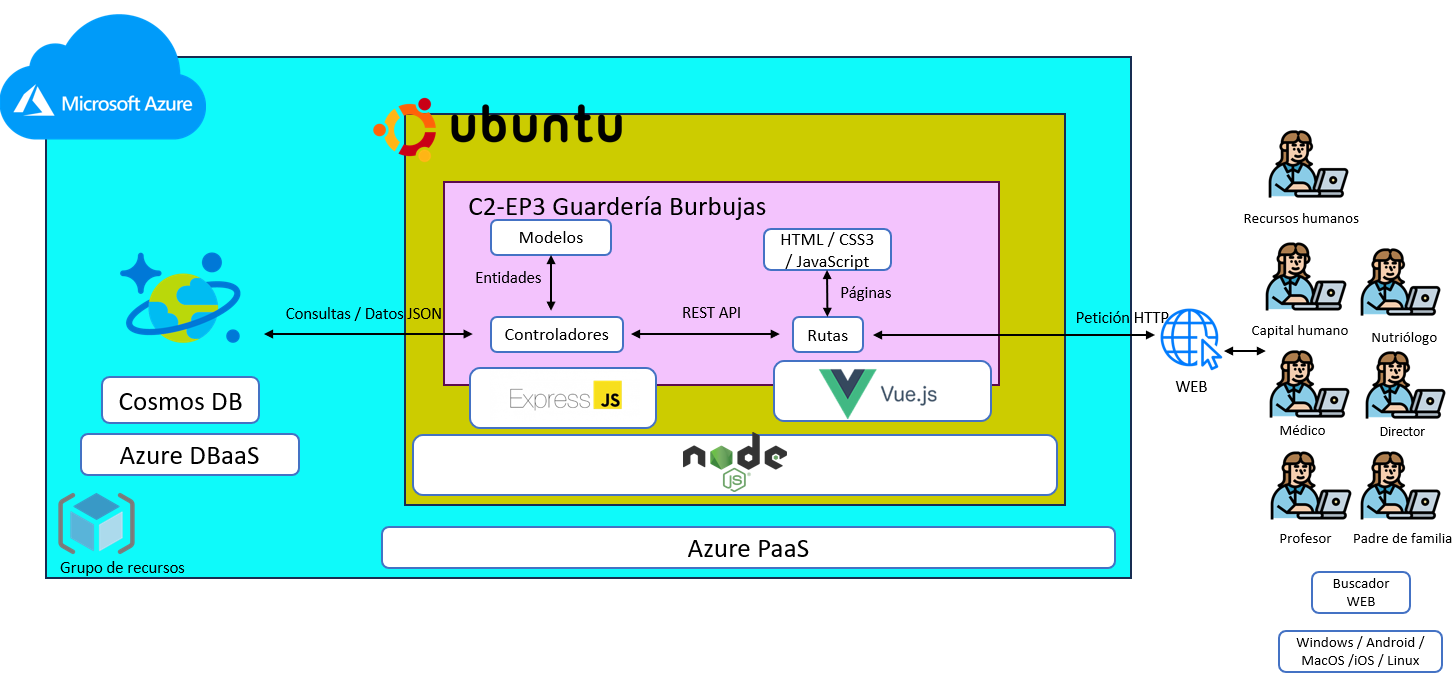
\includegraphics[width=0.9\textwidth]{images/arqui/plataforma.png}
\caption{Plataforma del sistema.}
\label{fig:plataforma}
\end{figure}

%---------------------------------------------------------
\section{Arquitectura.}	

Se puede considerar una arquitectura de tres capas que esta basado en la arquitectura del modelo vista controlador (MVC), que consiste en dividir la aplicación en capas lógicas distintas, cada una con su propósito y responsabilidades específicas. Estas capas son:

\begin{enumerate}
\item Capa de presentación o interfaz de usuario: Esta capa es responsable de la interacción con los usuarios finales y la presentación de la información de manera visualmente atractiva y fácil de usar. En este caso, Vue.js se encarga de construir la interfaz de usuario y proporcionar una experiencia interactiva al usuario. Esta capa también puede incluir la gestión de eventos del lado del cliente y la comunicación con el backend a través de API.

\item Capa de lógica de negocio: Esta capa contiene la lógica y reglas de negocio de la aplicación. Aquí es donde se procesan las solicitudes de los usuarios, se realizan operaciones en la base de datos y se aplican las reglas y validaciones necesarias. En la arquitectura MEVN stack, Express.js se encarga de construir el backend y manejar las solicitudes HTTP, las rutas y la lógica de negocio. En esta capa también se puede implementar la seguridad, la validación de datos y otras funcionalidades relacionadas con la lógica de negocio.

\item Capa de persistencia de datos: Esta capa se encarga del almacenamiento y acceso a los datos. Aquí es donde se interactúa con la base de datos para realizar operaciones de lectura y escritura. En el caso de este sistema, se utiliza Cosmos DB como la base de datos principal. Cosmos DB ofrece una integración nativa con Node.js y permite almacenar y consultar datos de manera eficiente y escalable. En esta capa también se pueden implementar estrategias de caché, gestión de transacciones y otros mecanismos relacionados con la persistencia de datos.

\end{enumerate}

La arquitectura de tres capas proporciona varios beneficios, como la separación de responsabilidades, la modularidad, la reutilización de código y la facilidad de mantenimiento. Cada capa puede desarrollarse y escalarse de forma independiente, lo que permite un desarrollo ágil y una mayor flexibilidad a medida que el sistema evoluciona.

En la Figura \ref{fig:arquitectura-tres-capas} se muestra una representación visual de la arquitectura de tres capas dentro del sistema.

\begin{figure}[htbp]
\centering
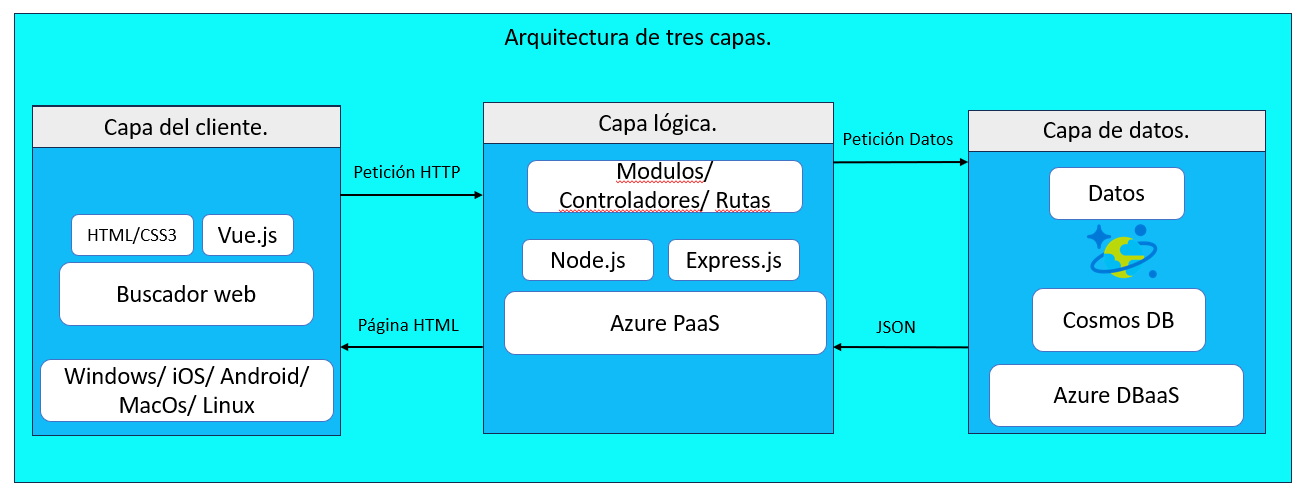
\includegraphics[width=0.9\textwidth]{images/arqui/3capas.png}
\caption{Arquitectura de tres capas en el sistema.}
\label{fig:arquitectura-tres-capas}
\end{figure}

La utilización de la arquitectura MEVN stack junto con la arquitectura de tres capas permite construir un sistema web robusto, escalable y modular. La combinación de estas tecnologías y enfoques arquitectónicos proporciona una base sólida para desarrollar y desplegar aplicaciones web modernas y eficientes en la nube de Azure.

%=========================================================
%=========================================================
\chapter{Modelo Estatico}	

En el diseño de sistemas de software, el enfoque modular es esencial para crear aplicaciones eficientes, mantenibles y escalables. El diseño de módulos se basa en la división del sistema en componentes más pequeños y autónomos, conocidos como módulos, que encapsulan funcionalidades específicas y se comunican entre sí de manera coherente. En el contexto del sistema de la guardería "Burbujas", el diseño de módulos desempeña un papel crucial en la organización y la implementación de las diversas características y procesos que son necesarios para su funcionamiento.

El objetivo del diseño de módulos en el sistema de la "Guardería burbujas" es garantizar una estructura clara y modular, donde cada módulo se encargue de una funcionalidad específica y pueda ser desarrollado, probado y mantenido de forma independiente. Esto permite una mayor flexibilidad en el desarrollo y facilita la colaboración entre el equipo de desarrollo. Además, el diseño de módulos promueve la reutilización de código, ya que los módulos pueden ser utilizados en diferentes partes del sistema o en proyectos futuros.
\\

Al diseñar los módulos del sistema de la "Guardería burbujas", se deben tener en cuenta diferentes aspectos, como la cohesión, la modularidad y la interoperabilidad. La cohesión se refiere a la medida en que los elementos dentro de un módulo están relacionados y trabajan juntos para cumplir una funcionalidad específica. Una alta cohesión indica que un módulo tiene una única responsabilidad y se centra en una tarea concreta. Por otro lado, la modularidad se refiere a la capacidad de un módulo de ser independiente y reemplazable sin afectar el funcionamiento de otros módulos. La interoperabilidad implica que los módulos deben poder comunicarse entre sí de manera eficiente y consistente, a través de interfaces bien definidas y protocolos de interacción.

%-----------------------------------------------------------------------
\section{Diseño de Subsistemas}

En el diseño de sistemas complejos, como es el caso del sistema de la guardería "Guardería Burbujas", se utiliza el concepto de subsistemas para organizar y estructurar las diferentes partes o componentes del sistema. Un subsistema es una unidad funcionalmente independiente dentro de un sistema más grande, que tiene la capacidad de realizar tareas específicas y contribuir al funcionamiento global del sistema.

Los subsistemas se utilizan para dividir un sistema en componentes más pequeños y manejables, lo cual facilita el diseño, la implementación y el mantenimiento del sistema en su conjunto. Cada subsistema tiene su propia funcionalidad y responsabilidades, y puede interactuar con otros subsistemas para lograr los objetivos del sistema en su conjunto.

El diseño de subsistemas implica identificar las diferentes partes o módulos del sistema que pueden funcionar de manera independiente pero también interactuar entre sí. Cada subsistema puede tener su propia arquitectura interna, sus interfaces con otros subsistemas y sus propias reglas y lógica de funcionamiento.

El diseño de subsistemas se basa en el principio de modularidad, que consiste en dividir un sistema en componentes más pequeños y cohesivos. Cada subsistema se enfoca en una funcionalidad específica y puede ser desarrollado y probado de manera independiente. Esto permite un desarrollo paralelo y una mayor reutilización de componentes en futuros proyectos.

En el contexto del sistema de la guardería "Guardería Burbujas", se pueden identificar varios subsistemas, como el subsistema de Gestion infantes, el subsistema de Gestión de padres de familia, el subsistema Gestión de días hábiles, el subsistema de Gestión de personal, el subsistema de Gestión de clases y el subsitema de Salud

\begin{figure}[htbp]
	\begin{center}
		\fbox{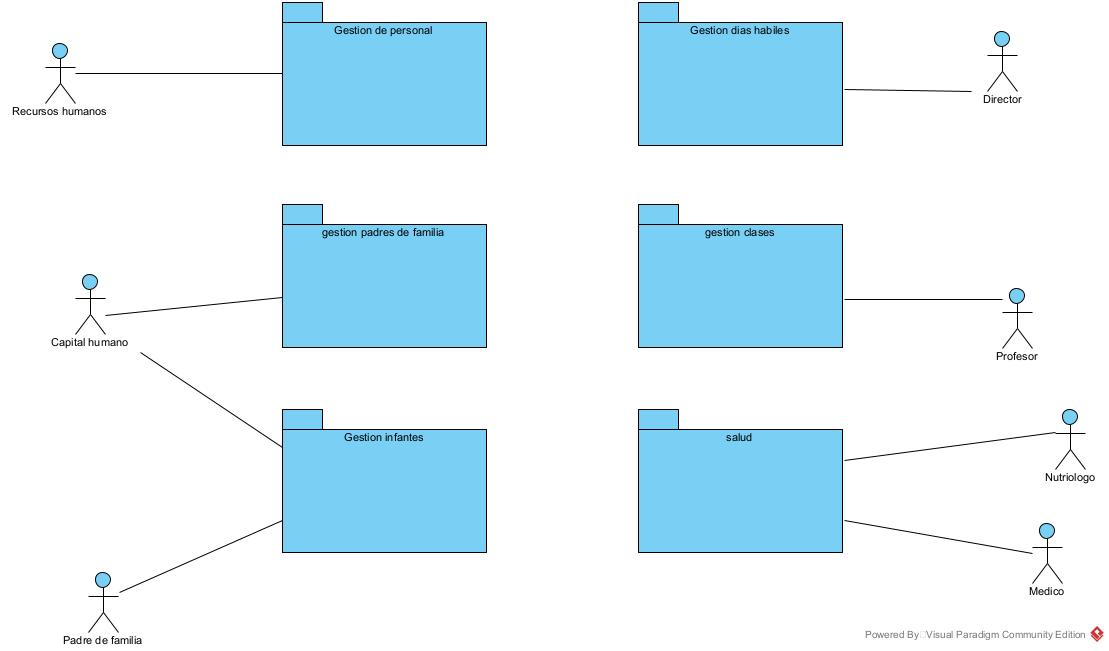
\includegraphics[width=.8\textwidth]{images/casosDeUso}}
		\caption{Diagrama de casos de uso del sistema.}
		\label{fig:casosDeUso}
	\end{center}
\end{figure}

Que son los subsitemas para los actores Recursos Humanos, Capital humano, Padre de familia, Médico, Nutriólogo, Director y Profesor.

\clearpage
%------------------------------------------------------------------
\subsection{Subsistema de Gestión de personal}
El personal de la guardería es un elemento clave para brindar un ambiente seguro, cuidadoso y estimulante para los niños. El subsistema de Gestión de Personal tiene como objetivo garantizar que se cuente con un equipo de profesionales capacitados y comprometidos, que cumplan con los requisitos de calificación necesarios y estén disponibles en los momentos adecuados para brindar atención y cuidado a los infantes.
\\
Este subsistema involucra diferentes actores, como el Director de la guardería, los Recursos Humanos y los propios miembros del personal. Cada actor desempeña un papel específico en la gestión del personal, desde la contratación y el proceso de selección hasta la asignación de tareas y la supervisión del rendimiento.

\begin{figure}[htbp]
\centering
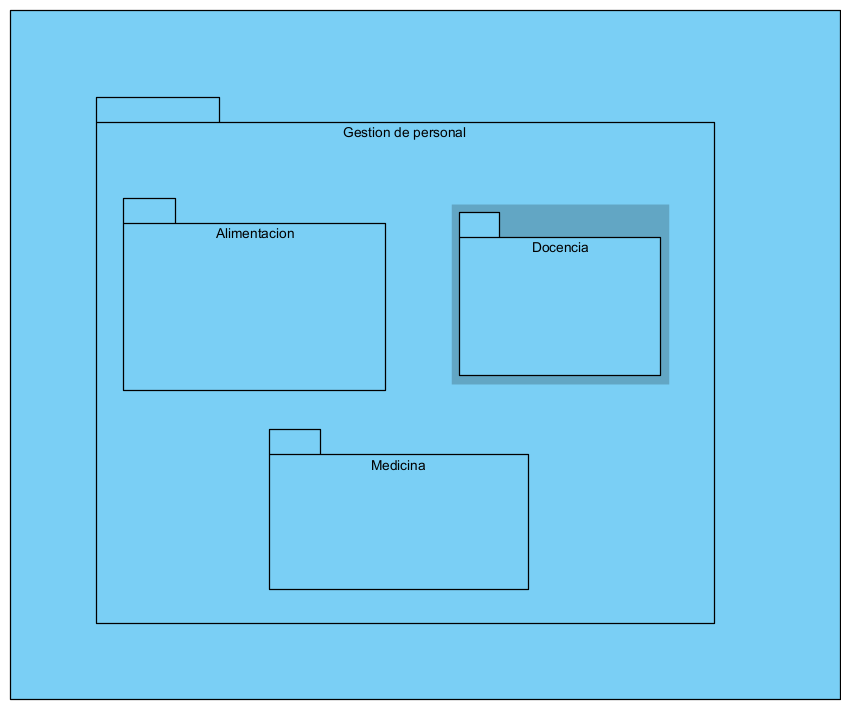
\includegraphics[width=0.7\textwidth]{images/arqui/subPersonal.png}
\caption{Subsistema Gestion de personal.}
\label{fig:subsistsalud}
\end{figure}

\subsubsection{Submódulo de Docencia}
El modulo "Docencia" es una parte integral del sistema de la guardería "Guardería Burbujas" y se encarga de gestionar todos los aspectos relacionados con el personal docente. Este módulo permite llevar un control eficiente del cuerpo docente, garantizando una educación de calidad y un entorno de aprendizaje óptimo para los niños.

El módulo de Docencia ofrece las siguientes funcionalidades:

\begin{itemize}
\item[*] Registro de profesor: Esta funcionalidad permite ingresar y almacenar la información relevante de los profesores que formarán parte del equipo docente de la guardería. Se recopilan datos como el nombre, la experiencia educativa, las especialidades y cualquier otra información necesaria para la asignación adecuada de los profesores a los grupos de niños.
\item[*] Dar de baja a profesor: En caso de que sea necesario, esta funcionalidad permite dar de baja a un profesor del sistema. Esto puede ocurrir por diversos motivos, como cambios en el personal, finalización de contrato o cualquier otra circunstancia que requiera la eliminación de un profesor del registro del sistema. Al dar de baja a un profesor, se actualiza la información de disponibilidad del personal docente.
\item[*] Actualización de datos del profesor: Esta funcionalidad permite realizar modificaciones y actualizaciones en la información de los profesores registrados. Puede incluir cambios en la información de contacto, actualización de experiencia educativa, incorporación de nuevas especialidades o cualquier otro dato relevante para mantener los registros del profesorado al día.
\end{itemize}

El módulo de Docencia es esencial para garantizar que el personal docente esté adecuadamente registrado, actualizado y asignado a los grupos de niños correspondientes. Esto facilita la planificación y organización de las clases, asegurando una distribución equitativa de los profesores y una atención de calidad en el proceso educativo de los infantes.

\begin{figure}[htbp]
\centering
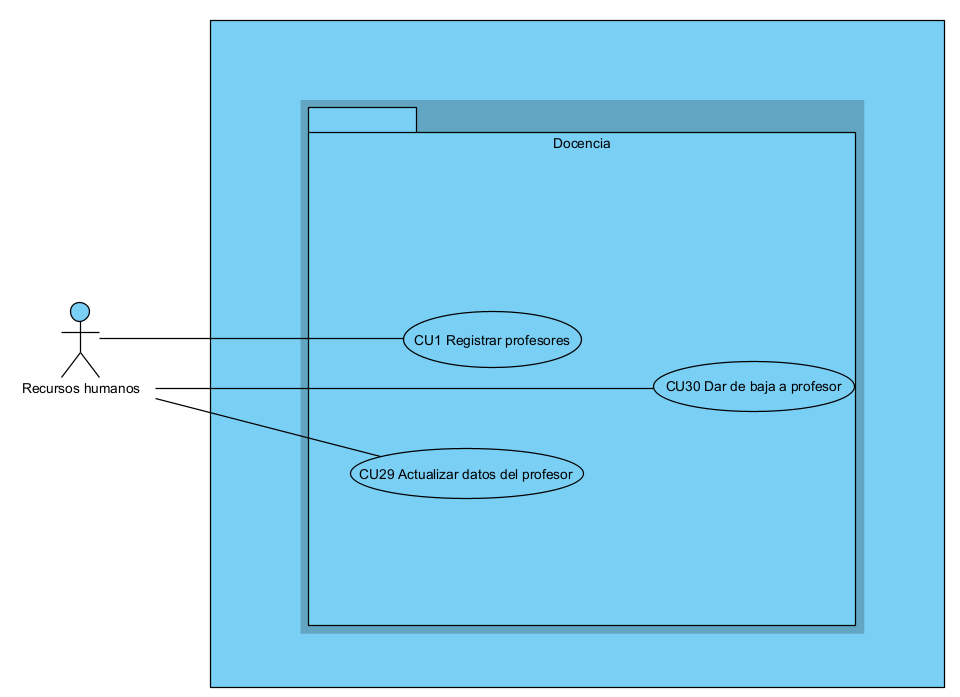
\includegraphics[width=0.7\textwidth]{images/arqui/subConsulDoce.png}
\caption{Modulo de Docencia del subsistema Gestion de personal.}
\label{fig:subsistGestDoce}
\end{figure}


\subsubsection{Submódulo de Alimentacion}

El módulo "Alimentacion" es una parte integral del sistema de la guardería "Guardería Burbujas" y se encarga de gestionar todos los aspectos relacionados con el personal de nutrición y alimentación. Este módulo permite llevar un control eficiente de los nutriólogos, asegurando una alimentación adecuada y equilibrada para los niños.

El módulo de Nutriólogo ofrece las siguientes funcionalidades:

\begin{itemize}
\item[*] Registro de nutriólogo: Esta funcionalidad permite ingresar y almacenar la información relevante de los nutriólogos que formarán parte del equipo encargado de la alimentación en la guardería. Se recopilan datos como el nombre, la experiencia en nutrición, las especialidades y cualquier otra información necesaria para la asignación adecuada de los nutriólogos a los grupos de niños.
\item[*] Dar de baja a nutriólogo: En caso de que sea necesario, esta funcionalidad permite dar de baja a un nutriólogo del sistema. Esto puede ocurrir por diversos motivos, como cambios en el personal, finalización de contrato o cualquier otra circunstancia que requiera la eliminación de un nutriólogo del registro del sistema. Al dar de baja a un nutriólogo, se actualiza la información de disponibilidad del personal de nutrición.
\item[*] Actualización de datos del nutriólogo: Esta funcionalidad permite realizar modificaciones y actualizaciones en la información de los nutriólogos registrados. Puede incluir cambios en la información de contacto, actualización de experiencia en nutrición, incorporación de nuevas especialidades o cualquier otro dato relevante para mantener los registros del personal de nutrición al día.
\end{itemize}


\begin{figure}[htbp]
\centering
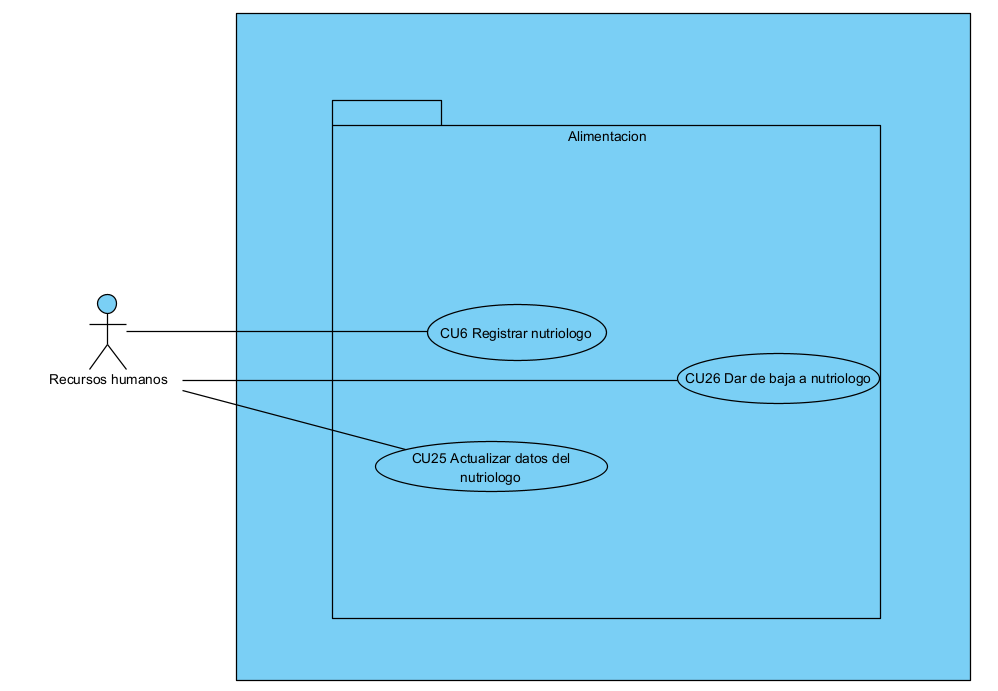
\includegraphics[width=0.7\textwidth]{images/arqui/subConsulAlimentac.png}
\caption{Modulo de Alimentacion del subsistema Gestion de personal.}
\label{fig:subsistGestalim}
\end{figure}


\subsubsection{Submódulo de Medicina}

El módulo "Medicina" es una parte integral del sistema de la guardería "Guardería Burbujas" y se encarga de gestionar todos los aspectos relacionados con el personal médico. Este módulo permite llevar un control eficiente de los médicos, asegurando la salud y el bienestar de los niños.

El módulo de Medicina ofrece las siguientes funcionalidades:

\begin{itemize}
\item[*] Registro de médico: Esta funcionalidad permite ingresar y almacenar la información relevante de los médicos que formarán parte del equipo médico de la guardería. Se recopilan datos como el nombre, la especialidad médica, la experiencia y cualquier otra información necesaria para la asignación adecuada de los médicos en el cuidado de los niños.
\item[*] Dar de baja a médico: En caso de que sea necesario, esta funcionalidad permite dar de baja a un médico del sistema. Esto puede ocurrir por diversos motivos, como cambios en el personal, finalización de contrato o cualquier otra circunstancia que requiera la eliminación de un médico del registro del sistema. Al dar de baja a un médico, se actualiza la información de disponibilidad del personal médico.
\item[*] Actualización de datos del médico: Esta funcionalidad permite realizar modificaciones y actualizaciones en la información de los médicos registrados. Puede incluir cambios en la información de contacto, actualización de especialidades médicas, incorporación de nuevas certificaciones o cualquier otro dato relevante para mantener los registros del personal médico al día.
\end{itemize}

El módulo de Medicina es esencial para garantizar que el personal médico esté adecuadamente registrado, actualizado y asignado a las tareas correspondientes. Esto facilita la atención médica de los niños, asegurando que reciban la atención adecuada en caso de enfermedades, lesiones u otras situaciones médicas que puedan surgir.


\begin{figure}[htbp]
\centering
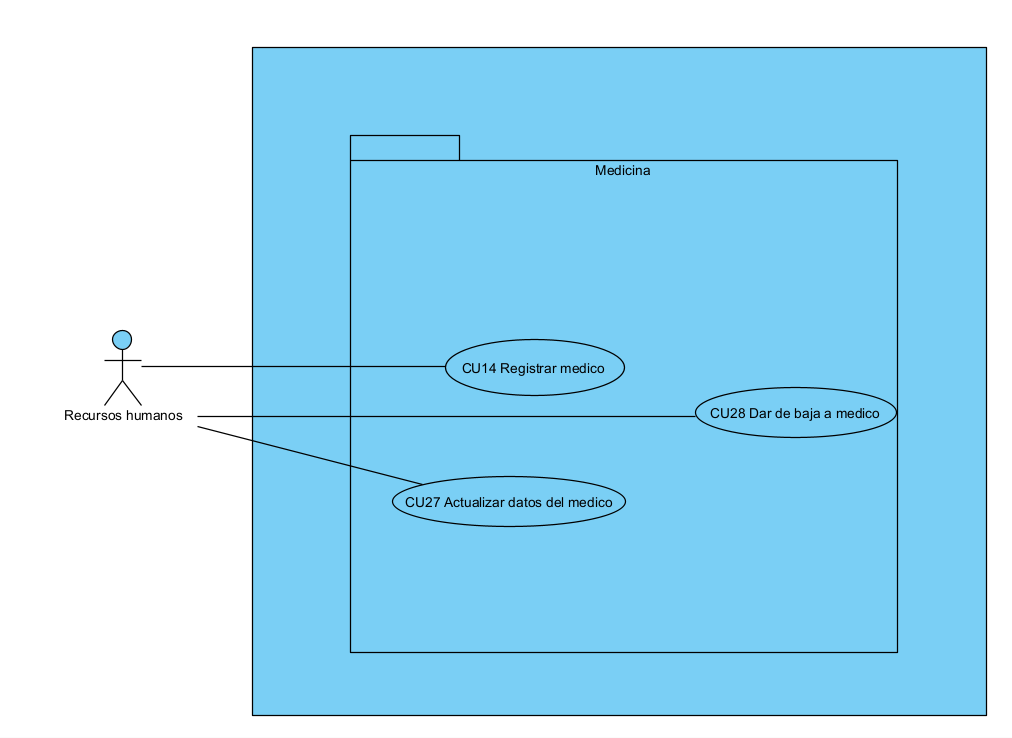
\includegraphics[width=0.7\textwidth]{images/arqui/subConsulMedicina.png}
\caption{Modulo de Medicina del subsistema Gestion de personal.}
\label{fig:subsistMedic}
\end{figure}

\clearpage
%------------------------------------------------------------------
\subsection{Subsistema de Gestión padres de familia}
El subsistema de "Gestión de padres de familia" es una parte esencial del sistema de la guardería "Guardería Burbujas". Este subsistema se encarga de administrar y mantener actualizada la información de los padres de familia de los infantes que asisten a la guardería. Su objetivo principal es tener la informacion de todos los padres de familia registrados para brindarles información relevante sobre sus hijos y garantizar una participación activa en el cuidado y desarrollo de los niños.

\begin{figure}[htbp]
\centering
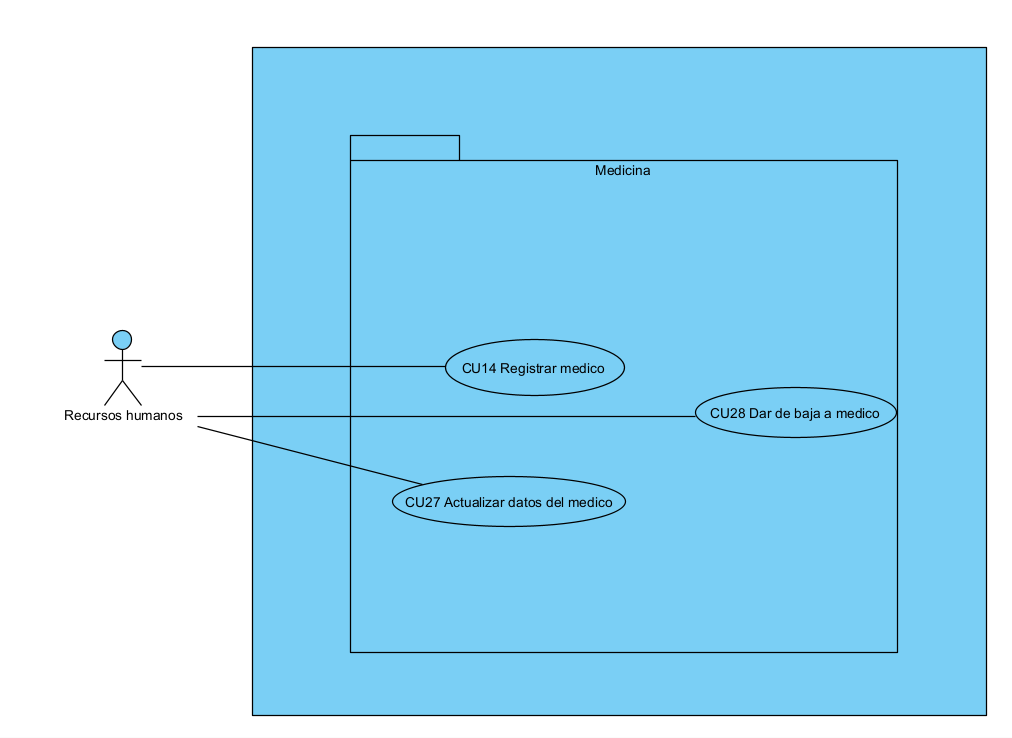
\includegraphics[width=0.7\textwidth]{images/arqui/subConsulMedicina.png}
\caption{Subsistema Gestion padres de familia.}
\label{fig:subsistGestionpapa}
\end{figure}
\clearpage
%------------------------------------------------------------------
\subsection{Subsistema de Gestión infantes}

El subsistema de "Gestión de infantes" es una parte fundamental del sistema de la guardería "Guardería Burbujas". Este subsistema se encarga de administrar y mantener actualizada la información de los infantes que asisten a la guardería, así como de supervisar su bienestar, progreso y desarrollo durante su estancia en el centro.


\begin{figure}[htbp]
\centering
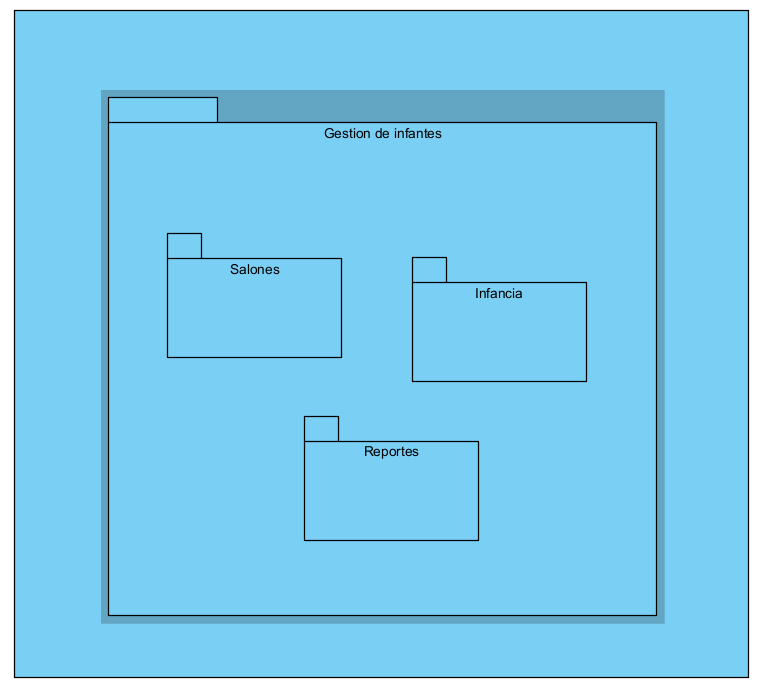
\includegraphics[width=0.7\textwidth]{images/arqui/subSisGestInfant.png}
\caption{Subsistema Gestion infantes.}
\label{fig:subsistGestionInfan}
\end{figure}

El subsistema de Gestión de infantes se divide en varios submódulos, que son los siguientes:

\subsubsection{Submódulo de salones}
El submódulo de salones tiene como objetivo principal organizar y administrar los diferentes salones de la guardería. En este submódulo se gestionan aspectos como la asignación de infantes a los salones correspondientes, la distribución equitativa de niños por grupo de edad y la supervisión de la capacidad máxima de cada salón. Además, se registran y actualizan datos relevantes de cada salón, como el nombre, la ubicación, los horarios y las actividades programadas.


\begin{figure}[htbp]
\centering
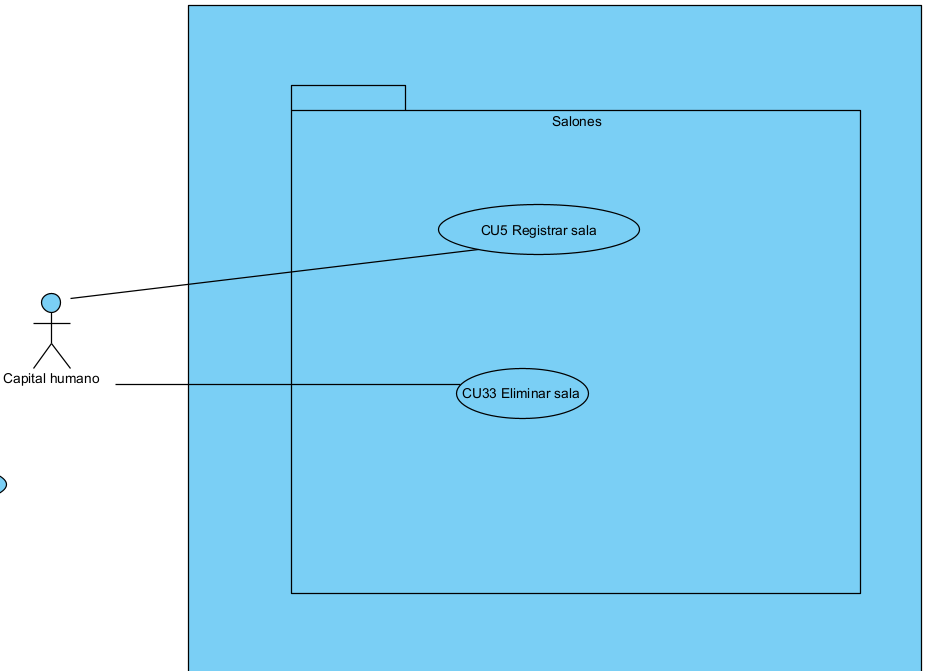
\includegraphics[width=0.7\textwidth]{images/arqui/subSisGestInfantSalon.png}
\caption{Diagrama del Submodulo de salones.}
\label{fig:subsistGestionInfansalones}
\end{figure}

\subsubsection{Submódulo de infancia}
El submódulo de infancia se encarga de recopilar y mantener actualizada la información personal y médica de cada infante. En este submódulo se registran datos como el nombre, la fecha de nacimiento, los contactos de emergencia, las alergias, las enfermedades crónicas y cualquier otra información relevante para brindar una atención adecuada y personalizada a cada niño. Además, se realiza un seguimiento del desarrollo y los hitos alcanzados por cada infante, lo que permite detectar y abordar oportunamente cualquier necesidad o preocupación.

\begin{figure}[htbp]
\centering
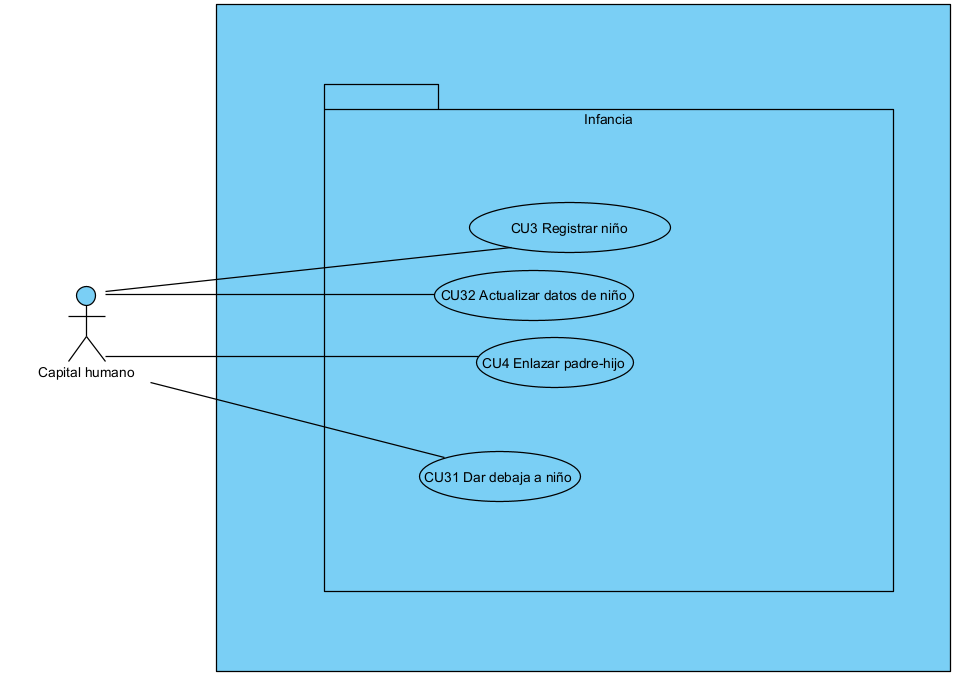
\includegraphics[width=0.7\textwidth]{images/arqui/subSisGestInfantInfancia.png}
\caption{Diagrama del Submodulo de infancia.}
\label{fig:subsistGestionInfanInfancia}
\end{figure}



\subsubsection{Submódulo de reportes}
El submódulo de reportes tiene como finalidad generar y proporcionar informes periódicos sobre el progreso y el bienestar de los infantes en la guardería. Estos informes incluyen aspectos como la asistencia, el desarrollo físico, emocional y cognitivo, las actividades realizadas, los logros alcanzados y cualquier otra información relevante. Estos reportes se comparten con los padres de familia y también pueden ser utilizados por el personal docente y administrativo para evaluar el desempeño de los infantes y realizar ajustes en los planes de atención y enseñanza.

\begin{figure}[htbp]
\centering
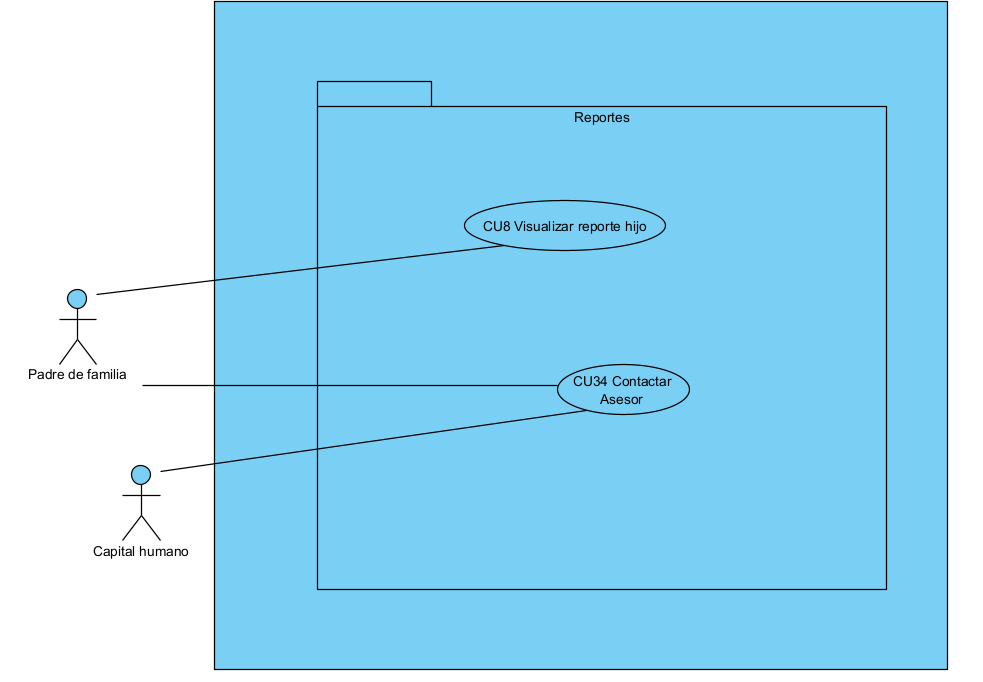
\includegraphics[width=0.7\textwidth]{images/arqui/subSisGestInfantReportes.png}
\caption{Diagrama del Submodulo de reportes.}
\label{fig:subsistGestionInfanReportes}
\end{figure}

\clearpage
%------------------------------------------------------------------
\subsection{Subsistema de Gestión días hábiles}

El subsistema de "Gestión de días hábiles" se encarga de administrar y gestionar los días hábiles, eventos escolares y días inhábiles en la guardería, con el objetivo de asegurar una planificación eficiente y un funcionamiento adecuado del centro.

El subsistema de Gestión de días hábiles consta de dos casos de uso directos, que son los siguientes:

\subsubsection{Registrar evento escolar}
Este caso de uso permite registrar y programar eventos escolares en el calendario de la guardería. Estos eventos pueden incluir actividades especiales, celebraciones, salidas educativas, visitas de invitados, entre otros. Al registrar un evento escolar, se asigna una fecha y se proporciona información relevante como la descripción, los horarios y las personas involucradas. Esto facilita la planificación y organización de las actividades, permitiendo que tanto el personal docente como los padres de familia estén informados y preparados para el evento.

\subsubsection{Registrar día inhábil}
Este caso de uso permite registrar y marcar como día inhábil aquellos días en los que la guardería no estará operativa. Estos días pueden corresponder a feriados, días de descanso programados, mantenimiento o cualquier otra circunstancia que requiera que el centro esté cerrado. Al registrar un día inhábil, se bloquea esa fecha en el calendario de la guardería, evitando la asignación de actividades y la presencia de personal y niños en el centro. Esto permite una gestión adecuada de los recursos y una planificación acorde a los días disponibles de funcionamiento.
\\
El subsistema de Gestión de días hábiles desempeña un papel crucial en la organización y planificación de la guardería "Guardería Burbujas". A través de los casos de uso de registrar eventos escolares y registrar días inhábiles, se establece un calendario que ayuda a mantener la coherencia y la eficiencia en el funcionamiento diario del centro. Esto garantiza que tanto el personal docente como los padres de familia estén al tanto de las actividades programadas y de los días en los que la guardería estará cerrada. En última instancia, este subsistema contribuye a crear un entorno estable y predecible para el desarrollo y cuidado de los infantes en la guardería.


\begin{figure}[htbp]
\centering
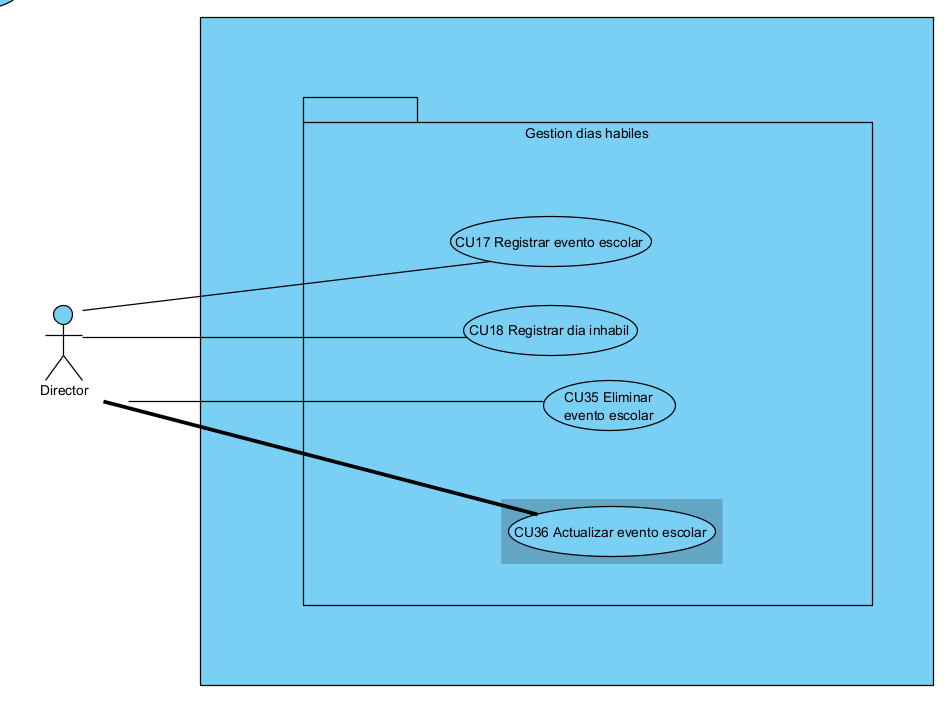
\includegraphics[width=0.7\textwidth]{images/arqui/subSisGestdias.png}
\caption{Diagrama del Subsistema de Gestion dias habiles.}
\label{fig:subsistGestiondias}
\end{figure}
\clearpage
%------------------------------------------------------------------
\subsection{Subsistema de Gestión clases}

El subsistema de "Gestión de clases" es una parte fundamental del sistema de la guardería "Guardería Burbujas". Este subsistema se encarga de la administración y control de las actividades relacionadas con las clases impartidas a los niños en la guardería. El objetivo principal de este subsistema es garantizar un ambiente educativo adecuado y facilitar el proceso de enseñanza-aprendizaje.

El subsistema de Gestión de clases consta de los siguientes submódulos:

\begin{itemize}
\item \textbf{Asistencia}: Este módulo permite realizar el registro y seguimiento de la asistencia de los niños a las clases. El profesor puede marcar la asistencia de cada estudiante y mantener un registro actualizado de su asistencia diaria. Esto facilita el control de la asistencia y proporciona información valiosa para evaluar la participación y el progreso de los niños en las actividades escolares.

\item \textbf{Reporte}: El módulo de Reporte permite generar informes y reportes sobre el desempeño y el progreso de los niños en las clases. El profesor puede ingresar datos relevantes, como calificaciones, observaciones y comentarios sobre el rendimiento de cada estudiante. Estos informes son útiles para evaluar el desarrollo de los niños, comunicarse con los padres y tomar decisiones educativas informadas.

\item \textbf{Avisos}: El módulo de Avisos es una herramienta de comunicación entre el profesor y los padres. Permite enviar notificaciones, recordatorios y mensajes importantes relacionados con las clases y el progreso de los niños. Los profesores pueden compartir información relevante, como fechas de eventos, tareas o cualquier otra comunicación necesaria para mantener una buena comunicación con los padres y garantizar su participación activa en la educación de sus hijos.

\end{itemize}

El actor principal que interactúa con el subsistema de Gestión de clases es el profesor. El profesor utiliza los diferentes módulos para tomar el control de las clases, registrar la asistencia de los niños, evaluar su desempeño y comunicarse de manera efectiva con los padres. A través de este subsistema, se busca promover un entorno educativo dinámico y propicio para el crecimiento y desarrollo de los niños en la guardería "Guardería Burbujas".


\begin{figure}[htbp]
\centering
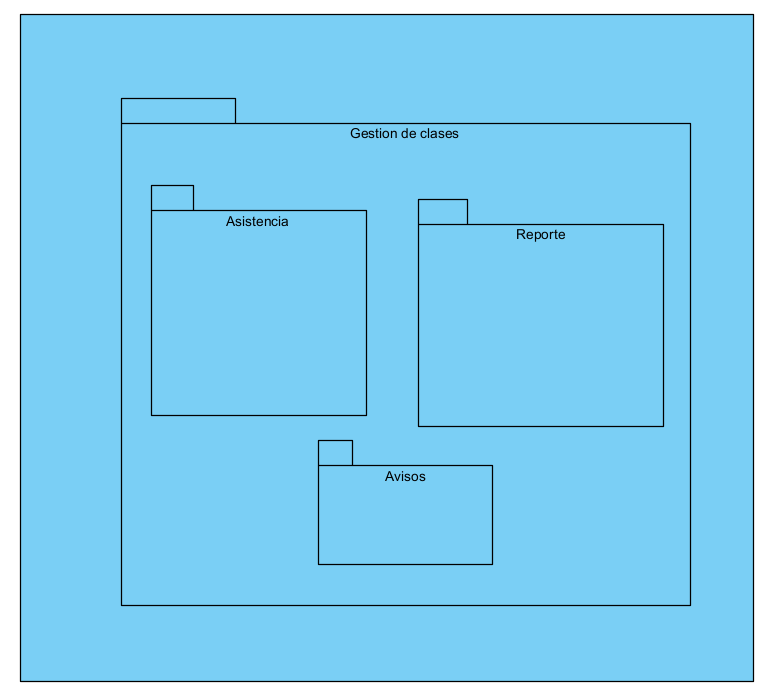
\includegraphics[width=0.7\textwidth]{images/arqui/subSisGestClases.png}
\caption{Diagrama del Subsistema de Gestion de Clases.}
\label{fig:subsistGestionClases}
\end{figure}

\subsubsection{Submódulo de Asistencia}

Este submódulo se encarga de realizar el registro y seguimiento de la asistencia de los niños a las clases, así como de registrar su salida al finalizar la jornada escolar. Su objetivo principal es mantener un control preciso y actualizado de la asistencia de los niños, lo que facilita la organización de las clases y proporciona información valiosa sobre su participación en las actividades escolares.

El submódulo de Asistencia ofrece las siguientes funcionalidades:

\begin{itemize}
\item \textbf{Tomar asistencia}: Esta funcionalidad permite al profesor tomar la asistencia de los niños al comienzo de cada clase. El profesor puede registrar la presencia o ausencia de cada estudiante, lo cual se refleja en el sistema. Esta información se utiliza para mantener un registro actualizado de la asistencia y generar informes precisos sobre la participación de los niños en las clases.

\item \textbf{Registrar salida}: Al finalizar la jornada escolar, el profesor puede registrar la salida de los niños en el submódulo de Asistencia. Esto asegura que se tenga un registro completo de las horas de asistencia de cada niño y brinda a los padres la tranquilidad de saber que sus hijos han sido debidamente registrados al ingresar y salir de la guardería.
\end{itemize}




\begin{figure}[htbp]
\centering
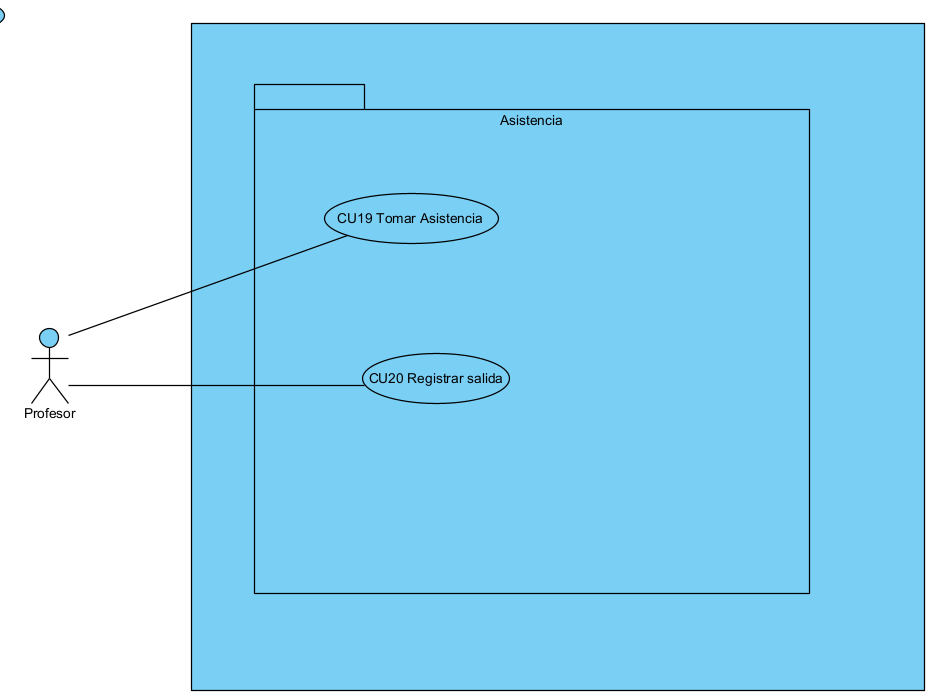
\includegraphics[width=0.7\textwidth]{images/arqui/subSisGestClasesAsis.png}
\caption{Diagrama del Submodulo de Asistencia.}
\label{fig:subsistGestionClasesAsis}
\end{figure}


\subsubsection{Submódulo de Avisos}

tiene como objetivo facilitar la comunicación entre el profesor y los padres de familia, brindando un canal eficiente para enviar y recibir avisos relevantes sobre actividades, eventos o cualquier otra información importante relacionada con la educación y el bienestar de los niños.

El submódulo de Avisos ofrece las siguientes funcionalidades:

\begin{itemize}
\item \textbf{Solicitar material}: Mediante esta funcionalidad, el profesor puede enviar avisos a los padres de familia solicitando materiales específicos para actividades escolares. Por ejemplo, si se va a realizar una manualidad, el profesor puede solicitar a los padres que envíen ciertos materiales como papel, pegamento, tijeras, entre otros. Esta funcionalidad agiliza el proceso de comunicación y permite al profesor asegurarse de contar con los recursos necesarios para llevar a cabo las actividades planificadas.

\item \textbf{Contactar padre de familia}: Esta funcionalidad permite al profesor establecer comunicación directa con los padres de familia para tratar asuntos específicos relacionados con los niños. Puede ser utilizada para compartir información personalizada, responder preguntas o resolver cualquier inquietud que pueda surgir. La capacidad de contactar directamente a los padres de familia a través del submódulo de Avisos fomenta una comunicación fluida y eficiente entre ambas partes, promoviendo una colaboración activa en la educación y cuidado de los niños.

\end{itemize}

\begin{figure}[htbp]
\centering
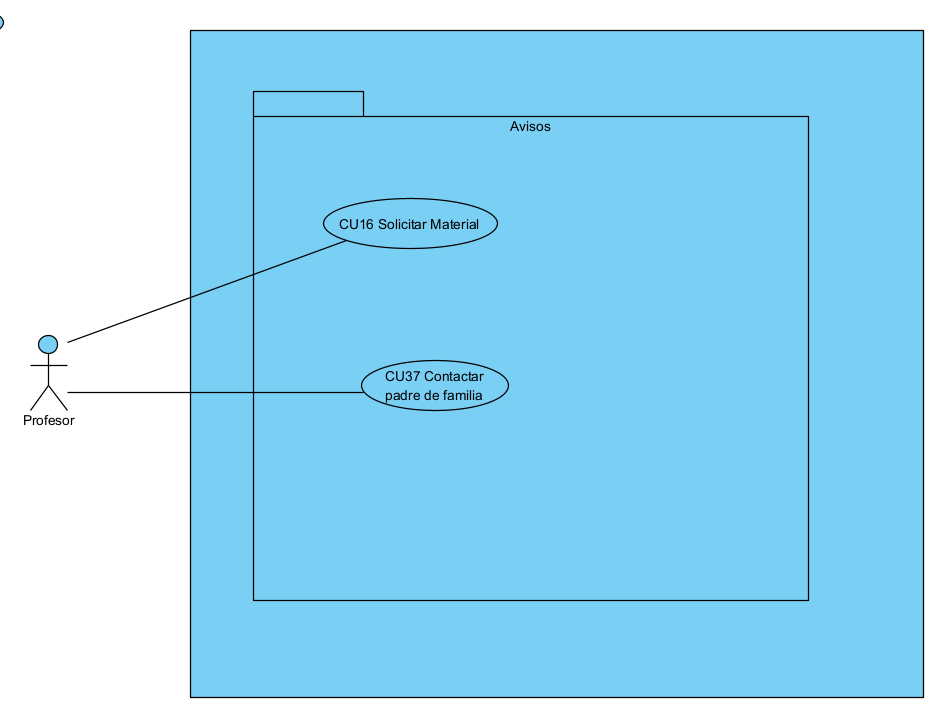
\includegraphics[width=0.7\textwidth]{images/arqui/subSisGestClasesAvis.png}
\caption{Diagrama del Submodulo de Avisos.}
\label{fig:subsistGestionClasesAvis}
\end{figure}

\subsubsection{Submódulo de Reportes}
El submódulo de Reportes es una parte esencial del subsistema de Gestión de clases en la guardería "Guardería Burbujas" se encarga de recopilar y registrar información relevante sobre diferentes aspectos relacionados con el cuidado y el desarrollo de los niños durante su estancia en la guardería.

El submódulo de Reportes ofrece las siguientes funcionalidades:

\begin{itemize}
\item \textbf{Registrar evacuaciones}: Esta funcionalidad permite al profesor registrar y documentar las evacuaciones realizadas por cada niño. Se registra información como la fecha, hora y características de la evacuación, lo cual es importante para llevar un control adecuado de la salud y bienestar de los infantes.

\item \textbf{Registrar ingesta}: Mediante esta funcionalidad, el profesor puede registrar la información sobre la ingesta de alimentos y bebidas de cada niño durante su estancia en la guardería. Se registra el tipo de alimento, la cantidad y cualquier otra observación relevante relacionada con la alimentación de los niños.

\item \textbf{Registrar cambio de ropa}: Esta funcionalidad permite al profesor registrar cualquier cambio de ropa que deba realizarse a un niño durante el día. Se registra la fecha, hora y motivo del cambio de ropa, lo cual es útil para mantener un seguimiento adecuado de las necesidades individuales de los niños.

\item \textbf{Registrar información adicional}: Esta funcionalidad permite al profesor registrar cualquier información adicional relevante sobre los niños. Puede incluir observaciones específicas, comportamientos destacados, eventos especiales o cualquier otra información que sea importante para comprender y atender las necesidades de los niños de manera individualizada.

\item \textbf{Generar reporte}: Una vez registrada la información en los submódulos anteriores, el profesor puede utilizar esta funcionalidad para generar un reporte consolidado. El reporte contiene un resumen de la información registrada en cuanto a evacuaciones, ingesta, cambios de ropa, información adicional, tareas y actividades realizadas por los niños. Estos reportes pueden ser utilizados para compartir información con los padres de familia, evaluar el progreso de los niños y realizar un seguimiento adecuado de su desarrollo.

\item \textbf{Registrar tareas y actividades}: Esta funcionalidad permite al profesor registrar las tareas y actividades que se realizan con los niños durante su estancia en la guardería. Se registra información como el tipo de tarea o actividad, la fecha, la duración y cualquier observación relevante. Esto facilita la planificación y organización de las actividades educativas y recreativas para el beneficio de los niños.

\end{itemize}

El submódulo de Reportes del subsistema de Gestión de clases juega un papel fundamental en la recopilación, registro y generación de información relevante sobre el cuidado y desarrollo de los niños en la guardería. Al utilizar este submódulo, se garantiza una documentación adecuada de las evacuaciones, la ingesta de alimentos, los cambios de ropa, la información adicional, las tareas y las actividades realizadas por los niños. Esto contribuye a la evaluación integral de su progreso, el seguimiento de sus necesidades individuales y la comunicación


\begin{figure}[htbp]
\centering
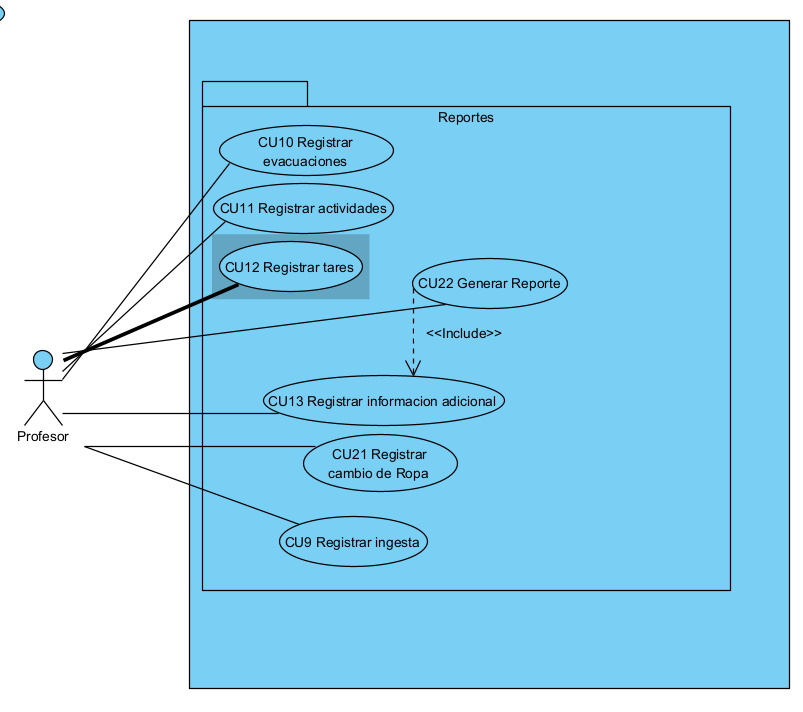
\includegraphics[width=0.7\textwidth]{images/arqui/subSisGestClasesRepor.png}
\caption{Diagrama del Submodulo de Reportes.}
\label{fig:subsistGestionClasesRepor}
\end{figure}


\clearpage
%------------------------------------------------------------------
\subsection{Subsistema Salud}

El subsistema de Salud es una parte fundamental del sistema de la guardería "Guardería Burbujas". Este subsistema se encarga de garantizar el bienestar y la salud de los niños que asisten a la guardería. En este subsistema, se involucran dos actores principales: el Médico y el Nutriólogo.\\

El Médico es responsable de llevar a cabo acciones relacionadas con la salud de los niños. Esto incluye generar consultas médicas, evaluar el estado de salud de los infantes, realizar diagnósticos, prescribir medicamentos y llevar un registro de las incidencias médicas de cada niño. El Médico juega un papel crucial en el cuidado y la atención médica de los niños, asegurándose de que estén sanos y respondiendo de manera adecuada a cualquier problema de salud que puedan presentar.

Por otro lado, el Nutriólogo desempeña un papel importante en el aspecto nutricional de los niños. Su tarea principal es crear los menús balanceados y adecuados para cada niño, teniendo en cuenta sus necesidades dietéticas individuales, alergias, preferencias y restricciones alimentarias. El Nutriólogo se asegura de proporcionar una alimentación saludable y equilibrada, promoviendo hábitos alimentarios saludables y fomentando el bienestar nutricional de los niños.

\begin{figure}[htbp]
\centering
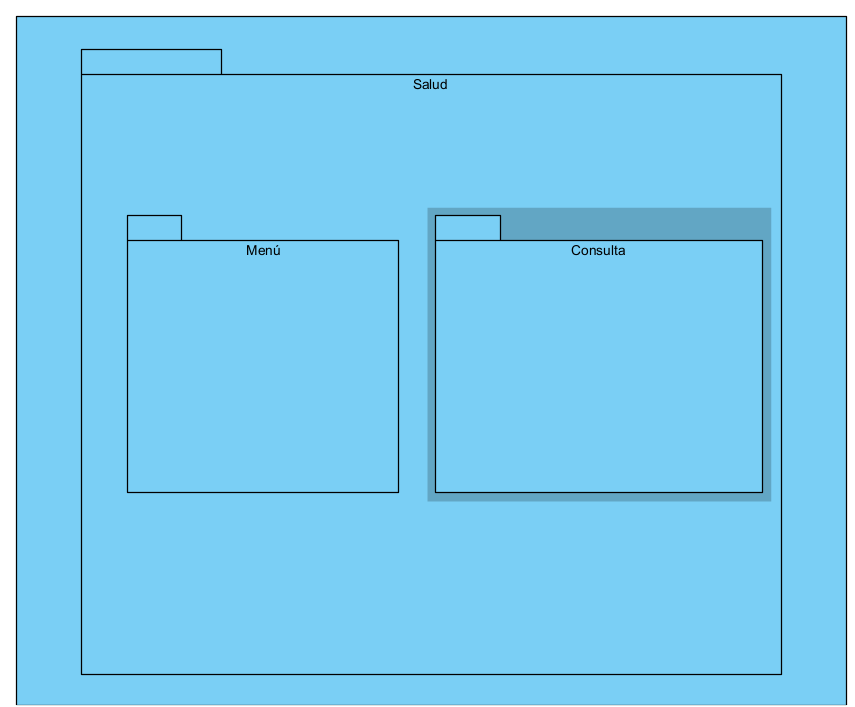
\includegraphics[width=0.7\textwidth]{images/arqui/subSalud.png}
\caption{Subsistema Salud.}
\label{fig:subsistsalud}
\end{figure}

\subsubsection{Submódulo de Menu}
La subsección "Menú" dentro del subsistema de Salud se encarga de gestionar las acciones relacionadas con la creación y registro de menús para los niños en la guardería "Guardería Burbujas". Este módulo es fundamental para garantizar una alimentación adecuada y equilibrada para los infantes, asegurando que se cumplan sus necesidades nutricionales.

El módulo del Menú permite realizar las siguientes acciones:

\begin{itemize}
    \item[*] Registro de menú: En esta funcionalidad, el nutriólogo encargado puede registrar los menús diarios o semanales para los diferentes grupos de niños. El nutriólogo puede seleccionar los alimentos adecuados y planificar las comidas de acuerdo con las necesidades nutricionales y restricciones dietéticas de cada niño.
    \item[*] Creación de menú especial: En algunos casos, es posible que se requiera crear menús especiales para niños con necesidades dietéticas específicas, como alergias o intolerancias alimentarias. El nutriólogo puede diseñar menús especiales adaptados a las necesidades individuales de cada niño, garantizando su seguridad y bienestar.
    \item[*] Visualización de menú: El nutriologo pueden acceder a la visualización de los menús registrados. Esta funcionalidad les permite planear de antemano las comidas que se servirán a los niños en la guardería, lo que les brinda tranquilidad y les permite tomar decisiones informadas sobre la alimentación de los infantes

\end{itemize}

\begin{figure}[htbp]
\centering
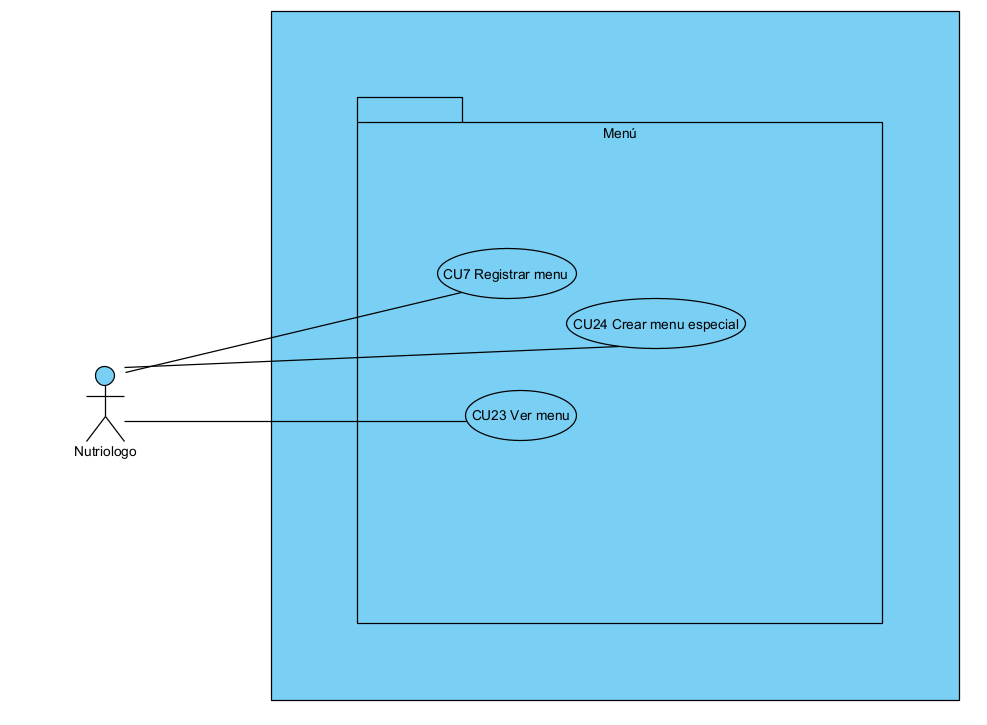
\includegraphics[width=0.7\textwidth]{images/arqui/subSaludMenu.png}
\caption{Modulo del Menu del subsistema Salud.}
\label{fig:subsistsaludmenu}
\end{figure}



\subsubsection{Submódulo de Consulta}
La subsección "Consulta" dentro del subsistema de Salud se encarga de gestionar las acciones relacionadas con la atención médica y el registro de incidencias médicas en la guardería "Guardería Burbujas". Este módulo es fundamental para asegurar el cuidado y bienestar de los niños, proporcionando un seguimiento adecuado de su estado de salud.

El módulo de Consulta permite realizar las siguientes acciones:

\begin{itemize}
\item[*] Registro de incidencia médica: En esta funcionalidad, el médico de la guardería puede registrar y documentar cualquier incidencia o situación médica que ocurra con un niño. Esto incluye enfermedades, lesiones, alergias u otras condiciones de salud relevantes. El médico puede ingresar detalles sobre el diagnóstico, tratamiento, medicamentos recetados y cualquier recomendación adicional para el cuidado del niño.


\end{itemize}

\begin{figure}[htbp]
\centering
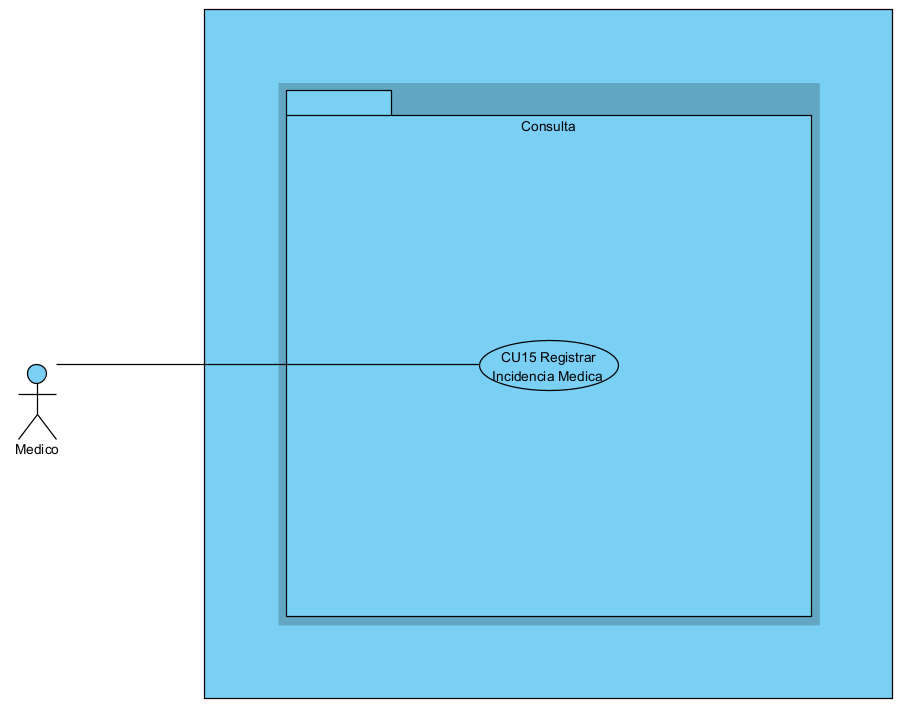
\includegraphics[width=0.7\textwidth]{images/arqui/subSaludConsulta.png}
\caption{Modulo de Consulta del subsistema Salud.}
\label{fig:subsistsaludcons}
\end{figure}
\clearpage


%==========================================================================
%-----------------------------------------------------------------------
\section{Diseño de clases}

El diseño de clases es una etapa esencial en el desarrollo de software basado en programación orientada a objetos (POO). En esta sección, nos centraremos en el diseño de clases relacionadas con diferentes entidades que forman parte de un sistema. Estas entidades incluyen a capital humano, los recursos humanos, los reportes, el menú de comidas, los padres de familia, los infantes, el director, el médico, el nutriólogo y el profesor.\\

En esta sección, abordaremos el diseño de clases para cada una de estas entidades, definiendo sus atributos, métodos y relaciones con otras clases. Un diseño de clases bien estructurado y coherente es fundamental para construir un sistema robusto y escalable, que cumpla con los requisitos y funcionalidades deseadas.


\begin{figure}[htbp]
\centering
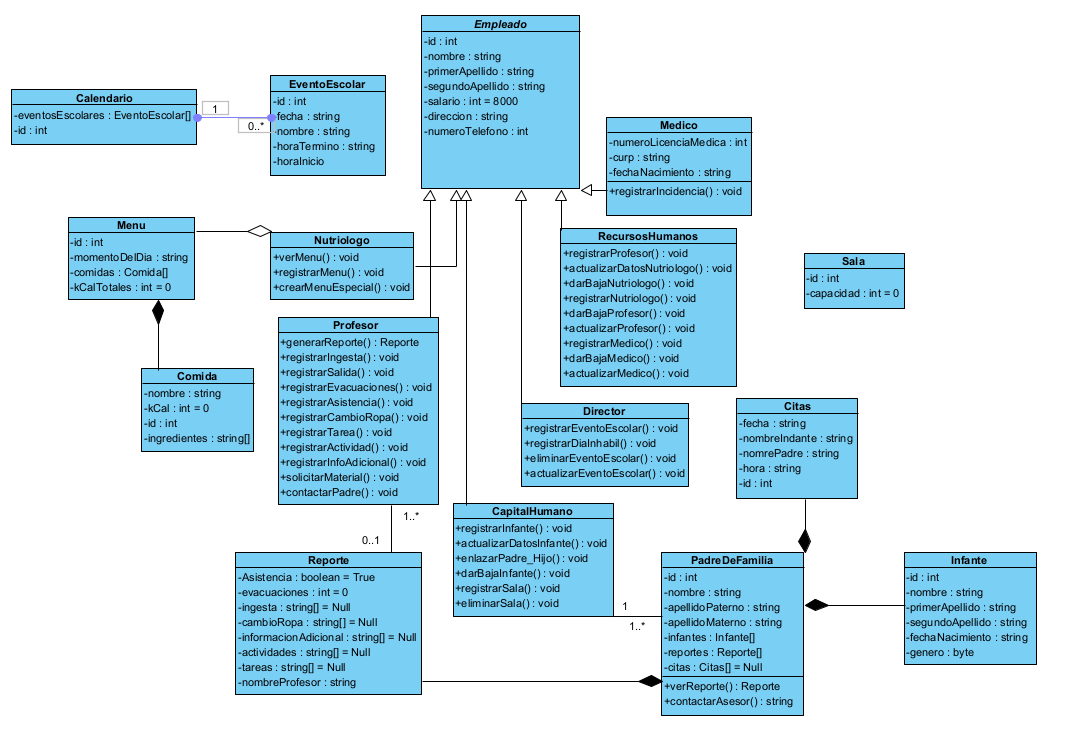
\includegraphics[width=0.9\textwidth]{images/arqui/entidades.png}
\caption{Diagrama de entidades del sistema.}
\label{fig:entidades}
\end{figure}
\clearpage

\subsection{Empleado}

En esta subsección, se aborda el diseño de la clase abstracta que representa a un empleado dentro del sistema. Un empleado es una entidad fundamental en cualquier organización y puede tener diferentes roles y responsabilidades. A continuación, se definen los atributos principales de la clase abstracta \texttt{Empleado}.

La clase abstracta \texttt{Empleado} contiene los siguientes atributos:

\begin{itemize}
\item \texttt{nombre}: Representa el nombre del empleado, que puede incluir su primer nombre o nombres.

\item \texttt{apellidoPaterno}: Indica el apellido paterno del empleado, que forma parte de su nombre completo.

\item \texttt{apellidoMaterno}: Representa el apellido materno del empleado, que también forma parte de su nombre completo.

\item \texttt{salario}: Indica la remuneración económica o sueldo que recibe el empleado por su trabajo.

\item \texttt{direccion}: Representa la ubicación física o geográfica donde el empleado desempeña sus funciones dentro de la organización.


\item \texttt{numeroTelefono}: Es el número de contacto telefónico del empleado, utilizado para comunicaciones y coordinación.

\item \texttt{id}: Es un identificador único asignado al empleado dentro del sistema, que se utiliza para realizar operaciones y realizar seguimiento de su información.

\end{itemize}

La clase abstracta \texttt{Empleado} se utiliza como base para definir clases más específicas que representan diferentes tipos de empleados en el sistema, como \texttt{Director}, \texttt{Medico}, \texttt{Nutriologo} y otros. Al ser una clase abstracta, no se puede instanciar directamente, pero proporciona una estructura común y atributos compartidos para las clases derivadas.

\begin{figure}[htbp]
\centering
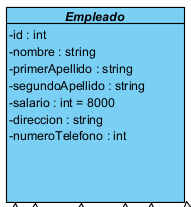
\includegraphics[width=0.4\textwidth]{images/arqui/empleado.png}
\caption{Diagrama de la clase abstracta empleado.}
\label{fig:entidadempleado}
\end{figure}
\clearpage
%------------------------------------------------------------------
\subsection{Nutriólogo}

La entidad \texttt{Nutriologo}, que es una subclase de la clase abstracta \texttt{Empleado}. El nutriólogo es un tipo específico de empleado que se especializa en la planificación y supervisión de la alimentación y nutrición de los infantes en la guardería "Guardería Burbujas".

La clase \texttt{Nutriologo} hereda los atributos de la clase \texttt{Empleado}, que incluyen:

\begin{itemize}
\item \textbf{nombre}: el nombre del nutriólogo.
\item \textbf{apellido paterno}: el apellido paterno del nutriólogo.
\item \textbf{apellido materno}: el apellido materno del nutriólogo.

\item \textbf{salario}: el salario del nutriólogo.
\item \textbf{ubicación}: la ubicación del nutriólogo en la guardería.

\item \textbf{número de teléfono}: el número de teléfono del nutriólogo.
\item \textbf{id}: el identificador único del nutriólogo en el sistema.
\end{itemize}

La clase \texttt{Nutriologo} también tiene los siguientes métodos:

\begin{itemize}
\item \textbf{verMenú()}: este método permite al nutriólogo ver el menú registrado para los infantes en la guardería. Proporciona al nutriólogo una visión general de las comidas planificadas y les permite realizar ajustes si es necesario.
\item \textbf{crearMenúEspecial()}: este método permite al nutriólogo crear un menú especial para un infante con necesidades dietéticas específicas, como alergias o intolerancias alimentarias. El nutriólogo puede diseñar un menú adaptado a las necesidades individuales del infante, asegurando una alimentación segura y saludable.
\item \textbf{registrarMenú()}: este método permite al nutriólogo registrar el menú diario o semanal para los infantes en la guardería. El nutriólogo puede seleccionar los alimentos adecuados y planificar las comidas de acuerdo con las necesidades nutricionales y restricciones dietéticas de cada infante.
\end{itemize}

La clase \texttt{Nutriologo} desempeña un papel fundamental en el subsistema de gestión de personal de la guardería "Guardería Burbujas". Con su experiencia y conocimientos en nutrición, contribuye a garantizar una alimentación adecuada y equilibrada para los infantes, promoviendo su bienestar y desarrollo saludable.


\begin{figure}[htbp]
\centering
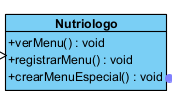
\includegraphics[width=0.4\textwidth]{images/arqui/nutriologo.png}
\caption{Diagrama de la clase anutriologo.}
\label{fig:entidadNutriologo}
\end{figure}

\clearpage
%------------------------------------------------------------------
\subsection{Medico}

La entidad \texttt{Médico}, que es una subclase de la clase abstracta \texttt{Empleado}. El médico es un tipo específico de empleado que brinda atención médica y cuidado de la salud a los infantes en la guardería "Guardería Burbujas".

La clase \texttt{Médico} hereda los atributos de la clase \texttt{Empleado}, que incluyen:

\begin{itemize}
\item \textbf{nombre}: el nombre del médico.
\item \textbf{apellido paterno}: el apellido paterno del médico.
\item \textbf{apellido materno}: el apellido materno del médico.

\item \textbf{salario}: el salario del médico.
\item \textbf{direccion}: la ubicación del médico en la guardería.

\item \textbf{número de teléfono}: el número de teléfono del médico.
\item \textbf{id }: el identificador único del médico en el sistema.
\end{itemize}

Además, la clase \texttt{Médico} tiene el atributo adicional:

\begin{itemize}
\item \textbf{numeroLicenciaMedica}: el número de licencia médica del médico, que identifica su autorización legal para ejercer la medicina.
\end{itemize}

La clase \texttt{Médico} también tiene el siguiente método:

\begin{itemize}
\item \textbf{registrarIncidencia()}: este método permite al médico registrar incidencias o eventos médicos relacionados con los infantes en la guardería. Puede incluir registros de enfermedades, lesiones o cualquier otra situación médica relevante. El médico puede proporcionar detalles y seguimiento adecuado para garantizar la salud y el bienestar de los infantes.
\end{itemize}

La clase \texttt{Médico} desempeña un papel crucial en el cuidado de la salud de los infantes en la guardería "Guardería Burbujas". Su experiencia médica y conocimientos permiten una atención adecuada en caso de enfermedad, lesiones o situaciones médicas imprevistas. Trabaja en estrecha colaboración con el personal y los padres de familia para garantizar un entorno seguro y saludable para los infantes.+

\begin{figure}[htbp]
\centering
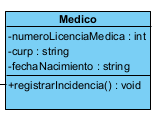
\includegraphics[width=0.4\textwidth]{images/arqui/medico.png}
\caption{Diagrama de la clase del Medico.}
\label{fig:entidadMedico}
\end{figure}

\clearpage
%------------------------------------------------------------------
\subsection{Profesor}
La entidad \texttt{Profesor}, que es una subclase de la clase abstracta \texttt{Empleado}. El profesor es un tipo específico de empleado que se encarga del cuidado y la educación de los infantes en la guardería "Guardería Burbujas".

La clase \texttt{Profesor} hereda los atributos de la clase \texttt{Empleado}, que incluyen:

\begin{itemize}
\item \textbf{nombre}: el nombre del profesor.
\item \textbf{apellido paterno}: el apellido paterno del profesor.
\item \textbf{apellido materno}: el apellido materno del profesor.

\item \textbf{salario}: el salario del profesor.
\item \textbf{direccion}: la ubicación del profesor en la guardería.

\item \textbf{número de teléfono}: el número de teléfono del profesor.
\item \textbf{id}: el identificador único del profesor en el sistema.
\end{itemize}

Además, la clase \texttt{Profesor} tiene los siguientes atributos adicionales:

\begin{itemize}
\item \textbf{registrarReporte}: este atributo representa la capacidad del profesor para registrar reportes sobre el progreso y el comportamiento de los infantes.
\item \textbf{registrarIngesta}: este atributo indica la capacidad del profesor para registrar la ingesta de alimentos de los infantes durante las comidas.
\item \textbf{registrarSalida}: este atributo permite al profesor registrar la hora de salida de los infantes al final del día.
\item \textbf{registrarEvacuaciones}: este atributo representa la capacidad del profesor para registrar las evacuaciones o visitas al baño de los infantes.
\item \textbf{registrarAsistencia}: este atributo indica la capacidad del profesor para registrar la asistencia de los infantes en la guardería.
\item \textbf{registrarCambioRopa}: este atributo permite al profesor registrar los cambios de ropa de los infantes, por ejemplo, después de actividades o en caso de accidentes.
\item \textbf{registrarTarea}: este atributo representa la capacidad del profesor para registrar las tareas asignadas a los infantes, como actividades de aprendizaje o tareas creativas.
\item \textbf{registrarActividad}: este atributo indica la capacidad del profesor para registrar las actividades realizadas por los infantes, como juegos, ejercicios o proyectos.
\item \textbf{registrarInfoAdicional}: este atributo permite al profesor registrar información adicional relevante sobre los infantes, como notas de comportamiento, preferencias o necesidades especiales.
\item \textbf{solicitarMaterial}: este atributo representa la capacidad del profesor para solicitar material o recursos necesarios para las actividades y el cuidado de los infantes.
\item \textbf{contactarPadre}: este atributo indica la capacidad del profesor para contactar a los padres de familia en caso de situaciones importantes, actualizaciones o consultas relacionadas con los infantes.
\end{itemize}

La clase \texttt{Profesor} desempeña un papel vital en el cuidado y la educación de los infantes en la guardería "Guardería Burbujas". Su responsabilidad incluye la supervisión, el apoyo y la instrucción de los infantes durante su estancia en la guardería. El profesor trabaja en estrecha colaboración con el personal y los padres de familia para garantizar el bienestar, el desarrollo y el aprendizaje de los infantes en un entorno seguro y estimulante.


\begin{figure}[htbp]
\centering
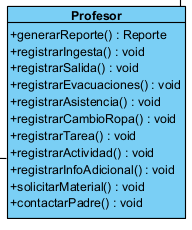
\includegraphics[width=0.4\textwidth]{images/arqui/profesor.png}
\caption{Diagrama de la clase del profesor.}
\label{fig:entidadProfesor}
\end{figure}

\clearpage
%------------------------------------------------------------------
\subsection{Capital Humano}

\texttt{CapitalHumano}, que es una subclase de la clase abstracta \texttt{Empleado}. La clase \texttt{CapitalHumano} se encarga de la gestión y administración de los recursos humanos relacionados con el cuidado de los infantes en la guardería "Guardería Burbujas".

La clase \texttt{CapitalHumano} hereda los atributos y métodos de la clase \texttt{Empleado}, y también tiene los siguientes métodos adicionales:

\begin{itemize}
\item \texttt{registrarInfante}: Este método permite registrar a un nuevo infante en el sistema. Se recopilan los datos necesarios del infante, como nombre, apellido, CURP, ubicación, edad, número de teléfono y ID en el sistema. Estos datos se utilizan para crear una nueva instancia de la clase \texttt{Infante} y agregarla al registro de infantes.

\item \texttt{actualizarDatosInfante}: Este método permite actualizar los datos de un infante registrado en el sistema. Se identifica al infante por su ID en el sistema y se actualizan los atributos correspondientes, como nombre, apellido, CURP, ubicación, edad y número de teléfono.

\item \texttt{enlazarPadre\_Hijo}: Este método permite establecer una relación entre un padre de familia y su hijo en el sistema. Se recopilan los datos del padre de familia y del infante, y se realiza el enlace correspondiente en el registro de padres e infantes.

\item \texttt{darBajaInfante}: Este método permite dar de baja a un infante del sistema. Se realiza mediante la identificación del infante por su ID en el sistema y eliminando su instancia correspondiente del registro de infantes.

\item \texttt{registrarSala}: Este método permite registrar una nueva sala en el sistema. Se recopilan los datos necesarios de la sala, como nombre, capacidad y ubicación, y se crea una nueva instancia de la clase \texttt{Sala} para agregarla al registro de salas.

\item \texttt{eliminarSala}: Este método permite eliminar una sala del sistema. Se realiza mediante la identificación de la sala por su ID en el sistema y eliminando su instancia correspondiente del registro de salas.
\end{itemize}

\begin{figure}[htbp]
\centering
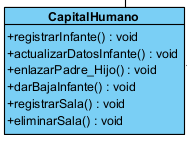
\includegraphics[width=0.4\textwidth]{images/arqui/capitalhumano.png}
\caption{Diagrama de la clase del Capital humano.}
\label{fig:entidadCaH}
\end{figure}

\clearpage
%------------------------------------------------------------------
\subsection{Director}

\texttt{Director}, que es una subclase de la clase abstracta \texttt{Empleado}. La clase \texttt{Director} representa al director de la guardería "Guardería Burbujas" y se encarga de la gestión y supervisión general de la institución.

La clase \texttt{Director} hereda los atributos y métodos de la clase \texttt{Empleado}, y también tiene los siguientes métodos adicionales:

\begin{itemize}
\item \texttt{registrarEventoEscolar}: Este método permite registrar un evento escolar en el sistema. Se recopilan los datos del evento, como el nombre, la fecha, la descripción y cualquier otra información relevante. El evento se agrega al registro de eventos escolares y se asocia con los infantes y el personal correspondiente.

\item \texttt{registrarDiaInhabil}: Este método permite registrar un día inhabil en el sistema. Se especifica la fecha y se agrega al registro de días inhabiles. Esto puede ser útil para planificar días en los que la guardería estará cerrada o no se ofrecerán servicios regulares.

\item \texttt{eliminarEventoEscolar}: Este método permite eliminar un evento escolar del sistema. Se realiza mediante la identificación del evento por su ID en el sistema y eliminando su instancia correspondiente del registro de eventos escolares.

\item \texttt{actualizarEventoEscolar}: Este método permite actualizar los datos de un evento escolar registrado en el sistema. Se identifica el evento por su ID en el sistema y se actualizan los atributos correspondientes, como el nombre, la fecha, la descripción y cualquier otra información relevante.

\end{itemize}



\begin{figure}[htbp]
\centering
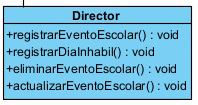
\includegraphics[width=0.4\textwidth]{images/arqui/director.png}
\caption{Diagrama de la clase director.}
\label{fig:entidadDirector}
\end{figure}

\clearpage
%------------------------------------------------------------------
\subsection{Recursos humanos}

\texttt{RecursosHumanos}, que es una subclase de la clase abstracta \texttt{Empleado}. La clase \texttt{RecursosHumanos} se encarga de la gestión y administración del personal en la guardería "Guardería Burbujas".

La clase \texttt{RecursosHumanos} hereda los atributos y métodos de la clase \texttt{Empleado}, y también tiene los siguientes métodos adicionales:

\begin{itemize}
\item \texttt{registrarProfesor}: Este método permite registrar a un nuevo profesor en el sistema. Se recopilan los datos necesarios del profesor, como nombre, apellido, CURP, salario, ubicación, edad, número de teléfono y ID en el sistema. Estos datos se utilizan para crear una nueva instancia de la clase \texttt{Profesor} y agregarla al registro de profesores.

\item \texttt{darBajaProfesor}: Este método permite dar de baja a un profesor del sistema. Se realiza mediante la identificación del profesor por su ID en el sistema y eliminando su instancia correspondiente del registro de profesores.

\item \texttt{actualizarDatosProfesor}: Este método permite actualizar los datos de un profesor registrado en el sistema. Se identifica al profesor por su ID en el sistema y se actualizan los atributos correspondientes, como nombre, apellido, CURP, salario, ubicación, edad y número de teléfono.

\item \texttt{actualizarDatosNutriologo}: Este método permite actualizar los datos de un nutriólogo registrado en el sistema. Se identifica al nutriólogo por su ID en el sistema y se actualizan los atributos correspondientes, como nombre, apellido, CURP, salario, ubicación, edad y número de teléfono.

\item \texttt{registrarNutriologo}: Este método permite registrar a un nuevo nutriólogo en el sistema. Se recopilan los datos necesarios del nutriólogo, como nombre, apellido, CURP, salario, ubicación, edad, número de teléfono y ID en el sistema. Estos datos se utilizan para crear una nueva instancia de la clase \texttt{Nutriologo} y agregarla al registro de nutriólogos.

\item \texttt{darBajaNutriologo}: Este método permite dar de baja a un nutriólogo del sistema. Se realiza mediante la identificación del nutriólogo por su ID en el sistema y eliminando su instancia correspondiente del registro de nutriólogos.

\item \texttt{actualizarDatosMedico}: Este método permite actualizar los datos de un médico registrado en el sistema. Se identifica al médico por su ID en el sistema y se actualizan los atributos correspondientes, como nombre, apellido, CURP, salario, ubicación, edad y número de teléfono.

\item \texttt{registrarMedico}: Este método permite registrar a un nuevo médico en el sistema. Se recopilan los datos necesarios del médico, como nombre, apellido, CURP, salario, ubicación, edad, número de teléfono y ID en el sistema. Estos datos se utilizan para crear una nueva instancia de la clase \texttt{Medico} y agregarla al registro de médicos.

\item \texttt{darBajaMedico}: Este método permite dar de baja a un médico del sistema. Se realiza mediante la identificación del médico por su ID en el sistema y eliminando su instancia correspondiente del registro de médicos.
\end{itemize}

\begin{figure}[htbp]
\centering
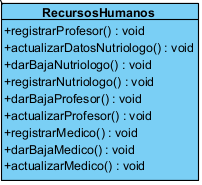
\includegraphics[width=0.4\textwidth]{images/arqui/recursoshumanos.png}
\caption{Diagrama de la clase recursos humanos.}
\label{fig:entidadRH}
\end{figure}

\clearpage
%------------------------------------------------------------------
\subsection{Padre de familia}
\texttt{Padre de familia}, que representa a los padres o tutores de los infantes inscritos en la guardería "Guardería Burbujas". Los padres de familia son parte integral del sistema y desempeñan un papel importante en la comunicación y el seguimiento del progreso de sus hijos.

La entidad \texttt{Padre de familia} tiene los siguientes atributos:

\begin{itemize}
\item \texttt{id}: Identificador único del padre de familia.
\item \texttt{nombre, apellidos}: El nombre y apellidos del padre de familia.
\item \texttt{infantes}: Una lista que contiene los infantes asociados a este padre de familia. Cada infante está representado por un objeto de la clase \texttt{Infante}.
\end{itemize}

Además, la entidad \texttt{Padre de familia} tiene los siguientes métodos:

\begin{itemize}
\item \texttt{verReporte}: Este método permite al padre de familia ver el reporte del progreso y desarrollo de sus infantes. El reporte puede incluir información sobre la asistencia, la alimentación, las actividades realizadas y cualquier otra observación relevante sobre el infante.

\item \texttt{contactarAsesor}: Este método permite al padre de familia contactar al asesor o profesor encargado del cuidado y educación del infante. El padre de familia puede utilizar este método para realizar consultas, programar reuniones o comunicar cualquier inquietud o necesidad relacionada con su hijo.

\end{itemize}

Estos métodos facilitan la interacción y comunicación entre los padres de familia y el personal de la guardería, promoviendo una colaboración efectiva en el cuidado y desarrollo de los infantes. Los atributos de la entidad \texttt{Padre de familia} permiten mantener un registro y una asociación adecuada entre los padres y sus hijos inscritos en la guardería.


\begin{figure}[htbp]
\centering
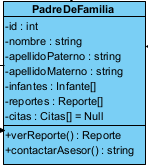
\includegraphics[width=0.4\textwidth]{images/arqui/padreFamilia.png}
\caption{Diagrama de la clase padre de familia.}
\label{fig:entidadpadre}
\end{figure}
\clearpage
%------------------------------------------------------------------
\subsection{Infante}
\texttt{Infante}, que representa a los niños inscritos en la guardería "Guardería Burbujas". Los infantes son el enfoque principal del sistema, ya que se centra en su cuidado, educación y bienestar.

La entidad \texttt{Infante} tiene los siguientes atributos:

\begin{itemize}
\item \texttt{id}: Identificador único del infante.
\item \texttt{nombre, apellidos}: El nombre y apellidos del infante.
\item \texttt{fechaNacimiento}: La fecha de nacimiento del infante.
\item \texttt{género}: El género del infante, que puede ser masculino, femenino o cualquier otra categoría aplicable.
\end{itemize}

Además de estos atributos, la entidad \texttt{Infante} puede tener otros atributos adicionales según las necesidades específicas del sistema, como información médica relevante, alergias, requerimientos especiales, entre otros.

No se especifican métodos específicos para la entidad \texttt{Infante} en esta descripción, ya que los métodos y funcionalidades relacionadas con el cuidado y la gestión de los infantes pueden ser implementados en las clases que heredan de esta entidad, como el \texttt{Profesor} o el \texttt{Padre de familia}.

\begin{figure}[htbp]
\centering
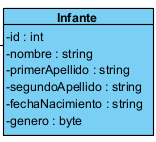
\includegraphics[width=0.4\textwidth]{images/arqui/infante.png}
\caption{Diagrama de la clase infante.}
\label{fig:entidadinfan}
\end{figure}


\begin{figure}[htbp]
\centering
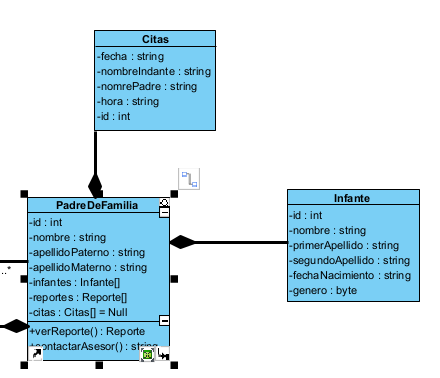
\includegraphics[width=0.4\textwidth]{images/arqui/colPadreFamilia.png}
\caption{Diagrama de la relacion del padre de familia con infantes.}
\label{fig:entidadpadin}
\end{figure}

\begin{figure}[htbp]
\centering
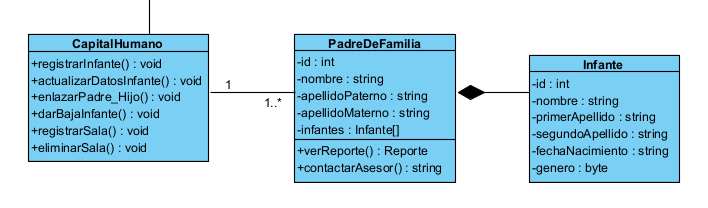
\includegraphics[width=0.4\textwidth]{images/arqui/capin.png}
\caption{Diagrama de la relacion de capital humano con padre e infantes.}
\label{fig:entidadpadin}
\end{figure}

\clearpage
%------------------------------------------------------------------
\subsection{Reporte}


\texttt{Reporte}, que representa un informe o registro de actividades y eventos relacionados con un infante en la guardería "Guardería Burbujas". Los reportes se utilizan para documentar diferentes aspectos del cuidado y el progreso del infante durante su estancia en la guardería.

La entidad \texttt{Reporte} tiene los siguientes atributos:

\begin{itemize}
\item \texttt{asistencia}: Registra la asistencia del infante a la guardería en un día específico.
\item \texttt{evacuaciones}: Registra las evacuaciones realizadas por el infante durante su estancia en la guardería, incluyendo información relevante como la frecuencia y características.
\item \texttt{ingesta}: Registra la información sobre la alimentación del infante, incluyendo la cantidad y tipo de alimentos consumidos.
\item \texttt{cambioRopa}: Registra los cambios de ropa realizados al infante, por ejemplo, en caso de accidentes o necesidades de higiene.
\item \texttt{informacionAdicional}: Permite registrar información adicional relevante sobre el infante, como observaciones especiales, necesidades particulares o eventos destacados.
\item \texttt{actividades}: Registra las actividades en las que el infante ha participado durante su jornada en la guardería, como juegos, ejercicios o tareas educativas.
\item \texttt{tareas}: Registra las tareas asignadas al infante para realizar en la guardería, como actividades de aprendizaje o responsabilidades específicas.
\item \texttt{nombreProfesor}: Almacena el nombre del profesor o encargado responsable de registrar el reporte del infante.
\end{itemize}


\begin{figure}[htbp]
\centering
\includegraphics[width=0.4\textwidth]{images/arqui/Reporte.png}
\caption{Diagrama de la clase reporte.}
\label{fig:entidadreporte}
\end{figure}

\begin{figure}[htbp]
\centering
\includegraphics[width=0.4\textwidth]{images/arqui/reprof.png}
\caption{Diagrama de la relacion del profesor y los reportes.}
\label{fig:entidadpadre}
\end{figure}


\clearpage
%------------------------------------------------------------------
\subsection{Menu y comidas}


Esta entidad \texttt{Menú} y se compone de la entidad \texttt{Comida} es importante para planificar y organizar las comidas ofrecidas a los infantes.

La entidad \texttt{Menú} tiene los siguientes atributos:

\begin{itemize}
\item \texttt{id}: Identificador único del menú.
\item \texttt{comidas}: Una lista de comidas que conforman el menú. Cada comida está representada por un objeto de la entidad \texttt{Comida}.
\item \texttt{momentoDelDia}: Indica el momento del día al que corresponde el menú, como desayuno, almuerzo o merienda.
\item \texttt{kCalTotales}: El total de calorías estimadas para todas las comidas del menú.
\end{itemize}

La entidad \texttt{Comida} representa una comida específica que forma parte del menú. Tiene los siguientes atributos:

\begin{itemize}
\item \texttt{id}: Identificador único de la comida.
\item \texttt{nombre}: Nombre de la comida.
\item \texttt{ingredientes}: Lista de ingredientes utilizados en la preparación de la comida.
\item \texttt{kCal}: Cantidad de calorías estimadas para la comida.
\end{itemize}

La entidad \texttt{Menú} se compone de varias instancias de la entidad \texttt{Comida}, lo que permite definir y organizar las opciones de alimentación para los infantes en la guardería. Cada comida tiene su propio conjunto de atributos, como nombre, ingredientes y calorías, lo que facilita la planificación de las comidas de acuerdo con los requisitos nutricionales y las preferencias alimenticias.

La entidad \texttt{Menú y Comidas} es esencial en el contexto de la guardería, ya que garantiza que se ofrezcan opciones de alimentación equilibradas y adecuadas para los infantes, promoviendo su salud y bienestar. Además, permite mantener un registro de los alimentos servidos y proporcionar información relevante a los padres de familia y al personal encargado de la alimentación.



\begin{figure}[htbp]
\centering
\includegraphics[width=0.4\textwidth]{images/arqui/menuComida.png}
\caption{Diagrama de la clase de Menu y de clase Comidas.}
\label{fig:entidamenucomida}
\end{figure}


\begin{figure}[htbp]
\centering
\includegraphics[width=0.4\textwidth]{images/arqui/comimennutr.png}
\caption{Diagrama de la relacion del menu con el nutriologo.}
\label{fig:entidamenucomida}
\end{figure}

\clearpage


%------------------------------------------------------------------
\subsection{Calendario y Eventos escolares.}

Para llevar un correcto manejo de los eventos escolares es que se usa un calendario, el cual se divide en dos entidades:
La entidad "Eventos Escolares" tiene los siguientes atributos:

\begin{itemize}
\item \textbf{ID:} Identificador único del evento escolar.
\item \textbf{Fecha:} Fecha en la que se llevará a cabo el evento escolar.
\item \textbf{Hora de Inicio:} Hora de inicio del evento escolar.
\item \textbf{Hora de Término:} Hora de término del evento escolar.
\item \textbf{Nombre:} Nombre o descripción del evento escolar.
\end{itemize}

La entidad "Calendario" tiene los siguientes atributos:

\begin{itemize}
\item \textbf{ID:} Identificador único del calendario.
\item \textbf{Eventos Escolares:} Un arreglo que almacena los eventos escolares programados en el calendario.
\end{itemize}


\begin{figure}[htbp]
\centering
\includegraphics[width=0.4\textwidth]{images/arqui/colCaEv.png}
\caption{Diagrama de la relacion Eventos Escolares con calendario}
\label{fig:colecEventCald}
\end{figure}

\clearpage


%------------------------------------------------------------------
\subsection{Salas.}

Las Salas son nuestras Salas en la guarderia, es por eso que es indispensable llevar un control de estas con su identificador y numero de capacidad.
La entidad "Sala" tiene los siguientes atributos:

\begin{itemize}
\item \textbf{ID:} Identificador único del evento escolar.
\item \textbf{Capacidad:} La capacidad maxima de esa sala
\end{itemize}


\begin{figure}[htbp]
\centering
\includegraphics[width=0.4\textwidth]{images/arqui/sala.png}
\caption{Diagrama de la entidad sala}
\label{fig:colecSala}
\end{figure}
\clearpage

%=========================================================
%=========================================================
\chapter{Modelo dinámico}	
\label{cap:modDinamico}

	Este capítulo describe en modelo dinámico del sistema. en el se detallan todos los escenarios de ejecución del sistema. La figura~\ref{fig:casosDeUso} muestra el diagrama general del sistema y sus sib sistemas, y la figura~\ref{fig:casosDeUsoDetalle} muestra todos los casos de uso del sistema. En este documento solo detallamos los casos de uso del subsistema de gestión de cursos.
	
\begin{figure}[htbp]
	\begin{center}
		\fbox{\includegraphics[width=.8\textwidth]{images/casosDeUso}}
		\caption{Diagrama de casos de uso del sistema.}
		\label{fig:casosDeUso}
	\end{center}
\end{figure}

\begin{figure}[htbp]
	\begin{center}
		\includegraphics[angle=90, width=.7\textwidth]{images/casosDeUsoDetalle}
		\caption{Diagrama detallado del sistema.}
		\label{fig:casosDeUsoDetalle}
	\end{center}
\end{figure}

%---------------------------------------------------------
\section{Descripción de actores}

%---------------------------------------------------------
\begin{Usuario}{\hypertarget{recursosHumanos}{\subsection{Recursos humanos}}}{
	Es el responsable de la gestion del personal dentro de la guarderia.
}
    \item[Responsabilidades:] \cdtEmpty
    \begin{itemize}
		\item Administrar la contratacion y despido del personal
		
    \end{itemize}

	\item[Perfil:] \cdtEmpty
    \begin{itemize}
		\item Licenciatura en recursos humanos, administracion de empresas o afin.
		\item un año de experiencia minimo en gestion de recursos humanos.
		\item Habilidades de liderazgo y trato humano.
    \end{itemize}
\end{Usuario}

\begin{Usuario}{\hypertarget{capitalHumano}{\subsection{Capital humano}}}{
	Es el encargado de la inscripcion de los infantes, asi como de recolectar la informacion de sus padres de familia
}
    \item[Responsabilidades:] \cdtEmpty
    \begin{itemize}
		\item Gestionar los expedientes de los infantes.
		\item Gestionar el estatus del infante dentro de la guarderia.
		\item Es el enlace entre los padres de familia y la guarderia.
    \end{itemize}

	\item[Perfil:] \cdtEmpty
    \begin{itemize}
		\item Licenciatura en trabajo social o afin.
		\item Experiencia en la gestion de documentacion de personas, preferiblemente ede               infantes.
		\item Tener un buen trato con las personas.
    \end{itemize}
\end{Usuario}

\begin{Usuario}{\hypertarget{medico}{\subsection{Médico}}}{
	Es el encargado de mantener la salud y el bienestar de los infantes en la guarderia.
}
    \item[Responsabilidades:] \cdtEmpty
    \begin{itemize}
		\item Supervisar la salud de los infantes.
		\item Proporcionar atencion medica a los infantes en caso de algun incidente.
		\item Proporcionar informacion sobre la salud de los infantes a sus padres.
    \end{itemize}

	\item[Perfil:] \cdtEmpty
    \begin{itemize}
		\item Titulo en medicina, preferiblemente con especialidad en pediatria.
		\item Licencia medica valida.
    \end{itemize}
\end{Usuario}

\begin{Usuario}{\hypertarget{nutriologo}{\subsection{Nutriologo}}}{
	Es el encargado de la buena alimentacion de los infantes.
}
    \item[Responsabilidades:] \cdtEmpty
    \begin{itemize}
		\item Diseñar un plan alimenticio para los infantes que sea saludable.
		\item Dar equivalencias de comida en caso de alergias.
    \end{itemize}

	\item[Perfil:] \cdtEmpty
    \begin{itemize}
		\item Licenciatura en alimentos o afin.
		\item Experiencia en nutricion pediatrica.
    \end{itemize}
\end{Usuario}

\begin{Usuario}{\hypertarget{director}{\subsection{Director}}}{
	Es la cabeza de la guarderia, es el encargado de la planeacion de los eventos.
}
    \item[Responsabilidades:] \cdtEmpty
    \begin{itemize}
		\item Creacion de eventos escolares.
		\item Gestiona los dias habiles de la guarderia.
    \end{itemize}

	\item[Perfil:] \cdtEmpty
    \begin{itemize}
		\item Maestria en el campo de la educacion.
    \end{itemize}
\end{Usuario}

\begin{Usuario}{\hypertarget{docente}{\subsection{Profesor}}}{
	Es el encargado de la educacion de los infantes, asi como de su cuidado.
}
    \item[Responsabilidades:] \cdtEmpty
    \begin{itemize}
		\item Supervisar a los infantes.
		\item Dar clases a los infantes.
		\item Dar informe a los padres de familia sobre el progreso de sus hijos y de su                  actividad academica.
            \item Llevar un registro de las comidas evacuaciones y cambios de ropa de los infantes
            \item Notificar sobre los materialies que se requieran para la realizacion de actividades.
    \end{itemize}

	\item[Perfil:] \cdtEmpty
    \begin{itemize}
		\item Titulo en pedagogia o afin.
		\item Experiencia en el cuidado de infantes.
    \end{itemize}
\end{Usuario}

\begin{Usuario}{\hypertarget{padre}{\subsection{Padre de familia}}}{
	Es el encargado legal del niño inscrito en la guarderia, recibe y proporciona informacion sobre el infante
}
    \item[Responsabilidades:] \cdtEmpty
    \begin{itemize}
		\item Llevar al niño a la guarderia a tiempo.
		\item Recoger al niño de la guarderia a tiempo.
		\item Brindar a la guarderia cambios de ropa para el niño.
            \item Asegurarse de la realizacion de actividades en casa del niño
            \item Llevar el material solicitado por la guarderia
    \end{itemize}

	\item[Perfil:] \cdtEmpty
    \begin{itemize}
		\item Es el responsable legal del niño.
		\item Responsabilidad.
    \end{itemize}
\end{Usuario}

A continuación se detallan los casos de uso.

%---------------------------------------------------------
% CASOS DE USO

% \IUref{IUAdmPS}{Administrar Planta de Selección}
% \IUref{IUModPS}{Modificar Planta de Selección}
% \IUref{IUEliPS}{Eliminar Planta de Selección}

% 


% Copie este bloque por cada caso de uso:
%-------------------------------------- COMIENZA descripción del caso de uso.

%\begin{UseCase}[archivo de imágen]{UCX}{Nombre del Caso de uso}{
%--------------------------------------
	\begin{UseCase}{CU1}{Registrar profesores}{
		Recursos humanos llenara los datos de un profesor para registrarla en el sistema.
	}
		\UCitem{Versión}{\color{Gray}0.1}
		\UCitem{Autor}{\color{Gray}Diego Rosas Cruz}
		\UCitem{Supervisa}{\color{Gray}Ulises Vélez Saldaña.}
		\UCitem{Actor}{\hyperlink{recursosHumanos}{Recursos humanos}}
		\UCitem{Propósito}{Se necesita registrar a los profesores para asignarlos a salas y luego asignar niños que vayan a tomar clase con cada uno de estos profesores.}
		\UCitem{Entradas}{nombre, dirección, no. de teléfono.}
		\UCitem{Origen}{Pantalla}
		\UCitem{Salidas}{MSGX.}
		\UCitem{Destino}{IUX}
		\UCitem{Precondiciones}{El profesor no debe estar registrado.}
		\UCitem{Postcondiciones}{Habrá un profesor nuevo registrado en el sistema.}
		\UCitem{Errores}{
            \begin{itemize}
                \item Si el profesor que intenta registar ya existe el sistema mostrará el mensaje de error y solicitará otra vez los datos.
                \item No se llenaron los datos correctamente; el sistema mostrara en que campos se tiene error y solicitara su corrección.
            \end{itemize}
            }
		\UCitem{Tipo}{Caso de uso primario}
		\UCitem{Observaciones}{ninguna}
	\end{UseCase}
%--------------------------------------
%--------------------------------------
	\begin{UCtrayectoria}
		\UCpaso[\UCactor] Accede al sistema.
		\UCpaso muestra la \IUref{IU4}{Pantalla principal Recursos Humanos}.
		\UCpaso[\UCactor] solicita registrar un profesor.
		\UCpaso muestra la \IUref{IUX}{Registrar Profesor}.
		\UCpaso[\UCactor] llena todos los datos solicitados para registrar un profesor.
		\UCpaso verifica que ese profesor no esté registrado\Trayref{A}.
		\UCpaso Verifica que todos los datos esten llenados correctamente \Trayref{B}.
		\UCpaso registra el nuevo profesor y muestra al actor el mensaje de éxito {\bf MSGX}:.
	\end{UCtrayectoria}
 %--------------------------------------		
		\begin{UCtrayectoriaA}{A}{El profesor ya existe}
			\UCpaso Muestra el Mensaje {\bf MSGX}``Ese profesor ya está registrado, por favor revise los datos.''.
			\UCpaso Continua en el paso 7 del caso de uso.
		\end{UCtrayectoriaA}
		
%--------------------------------------
		\begin{UCtrayectoriaA}{B}{Algun dato del formulario incorrecto}
			\UCpaso Muestra el Mensaje {\bf MSGX}``Revise los datos ingresados.''.
                \UCpaso Subraya de rojo los campos que tienen problemas con los datos ingresados.
			\UCpaso Continua en el paso 5 del caso de uso.
		\end{UCtrayectoriaA}

%-------------------------------------- TERMINA descripción del caso de uso.
% \IUref{IUAdmPS}{Administrar Planta de Selección}
% \IUref{IUModPS}{Modificar Planta de Selección}
% \IUref{IUEliPS}{Eliminar Planta de Selección}

% 


% Copie este bloque por cada caso de uso:
%-------------------------------------- COMIENZA descripción del caso de uso.

%\begin{UseCase}[archivo de imágen]{UCX}{Nombre del Caso de uso}{
%--------------------------------------
	\begin{UseCase}{CU2}{Registrar padre de familia}{
		Capital humano llenara los datos de un padre o tutor para registrarlo en el sistema.
	}
		\UCitem{Versión}{\color{Gray}0.1}
		\UCitem{Autor}{\color{Gray}Diego Rosas Cruz}
		\UCitem{Supervisa}{\color{Gray}Ulises Vélez Saldaña.}
		\UCitem{Actor}{\hyperlink{capitalHumano}{Capital humano}}
		\UCitem{Propósito}{Es necesario conocer al tutor o tutores de cada niño que entra en la guardería para poder notificarles cada que se requiera..}
		\UCitem{Entradas}{Nombre, dirección, no. de telefono.}
		\UCitem{Origen}{Pantalla}
		\UCitem{Salidas}{MSGX.}
		\UCitem{Destino}{IUX}
		\UCitem{Precondiciones}{El padre o tutor no debe estar registrado.}
		\UCitem{Postcondiciones}{Habrá un padre o tutor nuevo registrado en el sistema y uno o más niños se asignarán a este tutor.}
		\UCitem{Errores}{
            \begin{itemize}
                \item Si el tutor que intenta registar ya existe el sistema mostrará el mensaje de error y solicitará otra vez los datos.
                \item No se llenaron los datos correctamente; el sistema mostrara en que campos se tiene error y solicitara su corrección.
            \end{itemize}
            }
		\UCitem{Tipo}{Caso de uso primario}
		\UCitem{Observaciones}{ninguna}
	\end{UseCase}
%--------------------------------------
%--------------------------------------
	\begin{UCtrayectoria}
		\UCpaso[\UCactor] Accede al sistema.
		\UCpaso muestra la \IUref{IU5}{Pantalla principal Capital humano}.
		\UCpaso[\UCactor] solicita registrar un padre o tutor.
		\UCpaso muestra la \IUref{IUX}{Registrar Padre o tutor}.
		\UCpaso[\UCactor] llena todos los datos solicitados para registrar un padre o tutor.
		\UCpaso verifica que ese padre o tutor no esté registrado\Trayref{A}.
		\UCpaso Verifica que todos los datos esten llenados correctamente \Trayref{B}.
		\UCpaso registra el nuevo padre o tutor y muestra al actor el mensaje de éxito {\bf MSGX}:.
	\end{UCtrayectoria}
 %--------------------------------------		
		\begin{UCtrayectoriaA}{A}{El padre o tutor ya existe}
			\UCpaso Muestra el Mensaje {\bf MSGX}``Ese padre o tutor ya está registrado, por favor revise los datos.''.
			\UCpaso Continua en el paso 7 del caso de uso.
		\end{UCtrayectoriaA}
		
%--------------------------------------
		\begin{UCtrayectoriaA}{B}{Algun dato del formulario incorrecto}
			\UCpaso Muestra el Mensaje {\bf MSGX}``Revise los datos ingresados.''.
                \UCpaso Subraya de rojo los campos que tienen problemas con los datos ingresados.
			\UCpaso Continua en el paso 5 del caso de uso.
		\end{UCtrayectoriaA}

%-------------------------------------- TERMINA descripción del caso de uso.
% \IUref{IUAdmPS}{Administrar Planta de Selección}
% \IUref{IUModPS}{Modificar Planta de Selección}
% \IUref{IUEliPS}{Eliminar Planta de Selección}

% 


% Copie este bloque por cada caso de uso:
%-------------------------------------- COMIENZA descripción del caso de uso.

%\begin{UseCase}[archivo de imágen]{UCX}{Nombre del Caso de uso}{
%--------------------------------------
	\begin{UseCase}{CU3}{Registrar niño}{
		Capital humano llenará los datos de un niño para registrarlo en el sistema.
	}
		\UCitem{Versión}{\color{Gray}0.1}
		\UCitem{Autor}{\color{Gray}Diego Rosas Cruz}
		\UCitem{Supervisa}{\color{Gray}Ulises Vélez Saldaña.}
		\UCitem{Actor}{\hyperlink{capitalHumano}{Capital humano}}
		\UCitem{Propósito}{Es necesario tener los datos del niño en caso de que ocurra una incidencia, además los dos se requerien para tener al niño registrado en una sala, así como llevar un registro de todo lo relacionado con el niño.}
		\UCitem{Entradas}{Nombre, dirección, fecha de nacimiento.}
		\UCitem{Origen}{Pantalla}
		\UCitem{Salidas}{MSGX.}
		\UCitem{Destino}{IUX}
		\UCitem{Precondiciones}{El niño no debe estar registrado}
		\UCitem{Postcondiciones}{Habrá un niño nuevo registrado en el sistema.}
		\UCitem{Errores}{
            \begin{itemize}
                \item Si el niño que intenta registar ya existe el sistema mostrará el mensaje de error y solicitará otra vez los datos.
                \item No se llenaron los datos correctamente; el sistema mostrara en que campos se tiene error y solicitara su corrección.
            \end{itemize}
            }
		\UCitem{Tipo}{Caso de uso primario}
		\UCitem{Observaciones}{ninguna}
	\end{UseCase}
%--------------------------------------
%--------------------------------------
	\begin{UCtrayectoria}
		\UCpaso[\UCactor] Accede al sistema.
		\UCpaso muestra la \IUref{IU5}{Pantalla principal Capital humano}.
		\UCpaso[\UCactor] solicita registrar un niño.
		\UCpaso muestra la \IUref{IUX}{Registrar niño}.
		\UCpaso[\UCactor] llena todos los datos solicitados para registrar un niño.
		\UCpaso verifica que ese niño no esté registrado\Trayref{A}.
		\UCpaso Verifica que todos los datos esten llenados correctamente \Trayref{B}.
		\UCpaso registra el nuevo niño y muestra al actor el mensaje de éxito {\bf MSGX}:.
	\end{UCtrayectoria}
 %--------------------------------------		
		\begin{UCtrayectoriaA}{A}{El niño ya existe}
			\UCpaso Muestra el Mensaje {\bf MSGX}``Ese niño ya está registrado, por favor revise los datos.''.
			\UCpaso Continua en el paso 7 del caso de uso.
		\end{UCtrayectoriaA}
		
%--------------------------------------
		\begin{UCtrayectoriaA}{B}{Algun dato del formulario incorrecto}
			\UCpaso Muestra el Mensaje {\bf MSGX}``Revise los datos ingresados.''.
                \UCpaso Subraya de rojo los campos que tienen problemas con los datos ingresados.
			\UCpaso Continua en el paso 5 del caso de uso.
		\end{UCtrayectoriaA}

%-------------------------------------- TERMINA descripción del caso de uso.
% \IUref{IUAdmPS}{Administrar Planta de Selección}
% \IUref{IUModPS}{Modificar Planta de Selección}
% \IUref{IUEliPS}{Eliminar Planta de Selección}

% 


% Copie este bloque por cada caso de uso:
%-------------------------------------- COMIENZA descripción del caso de uso.

%\begin{UseCase}[archivo de imágen]{UCX}{Nombre del Caso de uso}{
%--------------------------------------
	\begin{UseCase}{CU4}{Enlazar padre hijo}{
		Capital humano enlazará cada niño con su padre o tutor.
	}
		\UCitem{Versión}{\color{Gray}0.1}
		\UCitem{Autor}{\color{Gray}Diego Rosas Cruz}
		\UCitem{Supervisa}{\color{Gray}Ulises Vélez Saldaña.}
		\UCitem{Actor}{\hyperlink{capitalHumano}{Capital humano}}
		\UCitem{Propósito}{Es necesario enlazar cada niño con su padre o tutor para saber a quién enviar avisos o llamar en caso de alguna incidencia con el niño.}
		\UCitem{Entradas}{IdNiño, IdPadre}
		\UCitem{Origen}{Pantalla}
		\UCitem{Salidas}{MSGX.}
		\UCitem{Destino}{IUX}
		\UCitem{Precondiciones}{El niño y el padre que serán enlazados tienen que estar registrados en la guardería.
  El niño no debe estar enlazado con más de dos tutores.
  El padre o tutor puede o no estar enlazado con otros niños.}
		\UCitem{Postcondiciones}{Un niño y un padre o tutor estarán enlazados en el sistema.}
		\UCitem{Errores}{
            \begin{itemize}
                \item El niño que se intenta enlazar ya está enlazado con dos tutores. El sistema mostrará un mensaje de error al enlazar.
            \end{itemize}
            }
		\UCitem{Tipo}{Caso de uso primario}
		\UCitem{Observaciones}{ninguna}
	\end{UseCase}
%--------------------------------------
%--------------------------------------
	\begin{UCtrayectoria}
		\UCpaso[\UCactor] Accede al sistema.
		\UCpaso muestra la \IUref{IU5}{Pantalla principal Capital humano}.
		\UCpaso[\UCactor] solicita enlazar un niño con un tutor,.
		\UCpaso muestra la \IUref{IUX}{Enlazar niño padre}.
		\UCpaso[\UCactor] Selecciona un padre
        \UCpaso[\UCactor] Selecciona un niño
		\UCpaso verifica que ese niño no esté enlazado con dos tutores.\Trayref{A}.
		\UCpaso enlaza al niño con el padre o tutor y muestra al actor el mensaje de éxito {\bf MSGX}:.
	\end{UCtrayectoria}
 %--------------------------------------		
		\begin{UCtrayectoriaA}{A}{El niño ya está enlazado con dos tutores.}
			\UCpaso Muestra el Mensaje {\bf MSGX}``Ese niño ya está enlazados con dos tutores, por favor escoja otro niño''.
			\UCpaso Continua en el paso 7 del caso de uso.
		\end{UCtrayectoriaA}

%-------------------------------------- TERMINA descripción del caso de uso.
% \IUref{IUAdmPS}{Administrar Planta de Selección}
% \IUref{IUModPS}{Modificar Planta de Selección}
% \IUref{IUEliPS}{Eliminar Planta de Selección}

% 


% Copie este bloque por cada caso de uso:
%-------------------------------------- COMIENZA descripción del caso de uso.

%\begin{UseCase}[archivo de imágen]{UCX}{Nombre del Caso de uso}{
%--------------------------------------
	\begin{UseCase}{CU5}{Registrar sala}{
		Capital humano llenara los datos de una sala para registrarla en el sistema.
	}
		\UCitem{Versión}{\color{Gray}0.1}
		\UCitem{Autor}{\color{Gray}Jose Angel Robles Otero}
		\UCitem{Supervisa}{\color{Gray}Ulises Vélez Saldaña.}
		\UCitem{Actor}{\hyperlink{capitalHumano}{Capital humano}}
		\UCitem{Propósito}{Se necesita tener registradas las salas existentes y su capacidad para saber cuantos menores más se pueden aceptar.}
		\UCitem{Entradas}{IdSala, capacidad.}
		\UCitem{Origen}{Pantalla}
		\UCitem{Salidas}{MSGX.}
		\UCitem{Destino}{IUX}
		\UCitem{Precondiciones}{La Sala no debe estar registrada.}
		\UCitem{Postcondiciones}{Habrá una sala más registrada en el sistema.}
		\UCitem{Errores}{
            \begin{itemize}
                \item Si la sala que intenta registrar ya existe el sistema mostrara el mensaje de error y solicitara otra vez los datos.
                \item No se llenaron los datos correctamente; el sistema mostrara en que campos se tiene error y solicitara su corrección.
            \end{itemize}
            }
		\UCitem{Tipo}{Caso de uso primario}
		\UCitem{Observaciones}{ninguna}
	\end{UseCase}
%--------------------------------------
	\begin{UCtrayectoria}
		\UCpaso[\UCactor] Accede al sistema.
		\UCpaso muestra la \IUref{IU5}{Pantalla principal Capital humano}.
		\UCpaso[\UCactor] solicita registrar una sala.
		\UCpaso muestra la \IUref{IU12}{Registrar sala}.
		\UCpaso[\UCactor] llena todos los datos solicitados para registrar una sala.
		\UCpaso verifica que no exista esa sala\Trayref{A}.
		\UCpaso Verifica que todos los datos esten llenados correctamente \Trayref{B}.
		\UCpaso registra la nueva sala y muestra al actor el mensaje de éxito {\bf MSGX}:.
	\end{UCtrayectoria}

%--------------------------------------		
		\begin{UCtrayectoriaA}{A}{La sala ya existe}
			\UCpaso Muestra el Mensaje {\bf MSGX}``Esa sala ya existe, favor de comprobar los datos de la sala a registrar.''.
			\UCpaso Continua en el paso 7 del caso de uso.
		\end{UCtrayectoriaA}
		
%--------------------------------------
		\begin{UCtrayectoriaA}{B}{Algun dato del formulario incorrecto}
			\UCpaso Muestra el Mensaje {\bf MSGX}``Revise los datos ingresados.''.
                \UCpaso Subraya de rojo los campos que tienen problemas con los datos ingresados.
			\UCpaso Continua en el paso 5 del caso de uso.
		\end{UCtrayectoriaA}

%-------------------------------------- TERMINA descripción del caso de uso.
% \IUref{IUAdmPS}{Administrar Planta de Selección}
% \IUref{IUModPS}{Modificar Planta de Selección}
% \IUref{IUEliPS}{Eliminar Planta de Selección}

% 


% Copie este bloque por cada caso de uso:
%-------------------------------------- COMIENZA descripción del caso de uso.

%\begin{UseCase}[archivo de imágen]{UCX}{Nombre del Caso de uso}{
%--------------------------------------
	\begin{UseCase}{CU6}{Registrar nutriólogo}{
		Recursos humanos registrará a un nuevo nutriólogo.
	}
		\UCitem{Versión}{\color{Gray}0.1}
		\UCitem{Autor}{\color{Gray}Diego Rosas Cruz}
		\UCitem{Supervisa}{\color{Gray}Ulises Vélez Saldaña.}
		\UCitem{Actor}{\hyperlink{recursosHumanos}{Recursos humanos}}
		\UCitem{Propósito}{Se necesita tener a cada nutriólogo registrado para saber quién está haciendo el menú en caso de que ocurra alguna incidencia.}
		\UCitem{Entradas}{nombre, dirección, numero de telefono.}
		\UCitem{Origen}{Pantalla}
		\UCitem{Salidas}{MSGX.}
		\UCitem{Destino}{IUX}
		\UCitem{Precondiciones}{El nutriólogo que se busca registrar no debe estar registrado en el sistema..}
		\UCitem{Postcondiciones}{Habrá un nuevo nutriólogo registrado en el sistema.}
	   \UCitem{Errores}{
            \begin{itemize}
                \item Si el nutriólogo que intenta registrar ya existe el sistema mostrará el mensaje de error y solicitará otra vez los datos.
                \item No se llenaron los datos correctamente; el sistema mostrara en que campos se tiene error y solicitara su corrección.
            \end{itemize}
            }
		\UCitem{Tipo}{Caso de uso primario}
		\UCitem{Observaciones}{ninguna}
	\end{UseCase}
%--------------------------------------
%--------------------------------------
	\begin{UCtrayectoria}
		\UCpaso[\UCactor] Accede al sistema.
		\UCpaso muestra la \IUref{IU4}{Pantalla principal Recursos humanos}.
		\UCpaso[\UCactor] solicita registrar nutriólogo
		\UCpaso muestra la \IUref{IUX}{Registrar nutriólogo}.
		\UCpaso[\UCactor] Ingresa datos del nutriólgo
		\UCpaso verifica que el nutriólogo no exista en el sistema..\Trayref{A}.
        \UCpaso Verifica que todos los datos estén llenados correctamente \Trayref{B}.
		\UCpaso registra un nuevo nutriólgo y muestra al actor el mensaje de éxito {\bf MSGX}:.
	\end{UCtrayectoria}
 %--------------------------------------		
		\begin{UCtrayectoriaA}{A}{El nutriólogo ya está registrado en el sistema.}
			\UCpaso Muestra el Mensaje {\bf MSGX}``Ese nutriólogo ya está registrado en el sistema, por favor ingrese los datos de un nuevo nutriólogo''.
			\UCpaso Continua en el paso 7 del caso de uso.
		\end{UCtrayectoriaA}
  %--------------------------------------
		\begin{UCtrayectoriaA}{B}{Algun dato del formulario incorrecto}
			\UCpaso Muestra el Mensaje {\bf MSGX}``Revise los datos ingresados.''.
                \UCpaso Subraya de rojo los campos que tienen problemas con los datos ingresados.
			\UCpaso Continua en el paso 5 del caso de uso.
		\end{UCtrayectoriaA}

%-------------------------------------- TERMINA descripción del caso de uso.
% Copie este bloque por cada caso de uso:
%-------------------------------------- COMIENZA descripción del caso de uso.

%\begin{UseCase}[archivo de imágen]{UCX}{Nombre del Caso de uso}{
%--------------------------------------
	\begin{UseCase}{CU7}{Registrar menú}{
		El nutriólogo llenara los datos de las comidas que se planean dar durante el mes y la fecha en que se planea que se den.
	}
		\UCitem{Versión}{\color{Gray}0.1}
		\UCitem{Autor}{\color{Gray}Jose Angel Robles Otero}
		\UCitem{Supervisa}{\color{Gray}Ulises Vélez Saldaña.}
		\UCitem{Actor}{\hyperlink{nutriologo}{Nutriologo}}
		\UCitem{Propósito}{Que los padres tengan conocimiento de las comidas que se le darán a los niños durante todo el mes.}
		\UCitem{Entradas}{NombrePlatillo, kCal, ingredientes, momentoComida.}
		\UCitem{Origen}{Pantalla}
		\UCitem{Salidas}{MSGX.}
		\UCitem{Destino}{Pantalla}
		\UCitem{Precondiciones}{la fecha de la comida a registrar debe ser posterior a la fecha del día de hoy}
		\UCitem{Postcondiciones}{Se visualizará en el calendario de comidas la comida registrada.}
		\UCitem{Errores}{{\bf 1}: Si la fecha de la comida a registrar es la del día de hoy o alguna anterior, se mostrara el mensaje Err2 y se solicitara que cambie ese dato
        \newline
  
	{\bf 2}: No se llenaron los datos correctamente; el sistema mostrara        en que campos se tiene error y solicitara su corrección.
        \newline
 
        {\bf 3}: Si la fecha y momento del dia de la comida a registrar coinciden con los de alguna comida ya registrada, el sistema dará la opción de modificar la comida ya registrada o de cambiar la comida por registrar a través del mensaje msg3}
		\UCitem{Tipo}{Caso de uso primario}
		\UCitem{Observaciones}{ninguna}
	\end{UseCase}
%--------------------------------------
	\begin{UCtrayectoria}
		\UCpaso[\UCactor] Accede al sistema.
		\UCpaso muestra la \IUref{IU1}{pantalla principal del nutriologo} .
		\UCpaso[\UCactor] solicita registrar una comida.
		\UCpaso muestra la \IUref{IU14}{Pantalla de Registro de comidas} .
		\UCpaso[\UCactor] llena todos los datos solicitados para registrar una comida.
            \UCpaso verifica que todos los datos fueron llenados y que son del tipo que corresponde. \Trayref{A}.
		\UCpaso verifica que la fecha ingresada sea posterior a la de hoy \Trayref{B}.
		\UCpaso verifica que no exista una comida en el mismo dia y al mismo momento. \Trayref{C}.
		\UCpaso registra la comida y muestra el menú de comidas.
	\end{UCtrayectoria}



%--------------------------------------
		\begin{UCtrayectoriaA}{A}{Algun dato del formulario incorrecto}
			\UCpaso Muestra el Mensaje {\bf MSGX}``Revise los datos ingresados.''.
                \UCpaso Subraya de rojo los campos que tienen problemas con los datos ingresados.
			\UCpaso Continua en el paso 5 del caso de uso.
		\end{UCtrayectoriaA}


%--------------------------------------		
            \begin{UCtrayectoriaA}{B}{La fecha de la comida es hoy o antes de hoy}
			\UCpaso Muestra el Mensaje {\bf MSGX}``La fecha de la comida debe ser porterior a la fecha del dia de hoy.''.
			\UCpaso Continua en el paso 5 del caso de uso.
		\end{UCtrayectoriaA}
		
%--------------------------------------
		\begin{UCtrayectoriaA}{C}{La comida ya existe}
			\UCpaso Muestra el Mensaje {\bf MSGX}``Esa comida ya estaba registrada, asegurece de que ingreso la fecha bien.''.
			\UCpaso Continua en el paso 5 del caso de uso.
		\end{UCtrayectoriaA}

%-------------------------------------- TERMINA descripción del caso de uso.
% \IUref{IUAdmPS}{Administrar Planta de Selección}
% \IUref{IUModPS}{Modificar Planta de Selección}
% \IUref{IUEliPS}{Eliminar Planta de Selección}

% 


% Copie este bloque por cada caso de uso:
%-------------------------------------- COMIENZA descripción del caso de uso.

%\begin{UseCase}[archivo de imágen]{UCX}{Nombre del Caso de uso}{
%--------------------------------------
	\begin{UseCase}{CU8}{Generar cita}{
		El director, un nutriólogo, profesor o médico pueden generar una cita con los tutores.
	}
		\UCitem{Versión}{\color{Gray}0.1}
		\UCitem{Autor}{\color{Gray}Diego Rosas Cruz}
		\UCitem{Supervisa}{\color{Gray}Ulises Vélez Saldaña.}
		\UCitem{Actor}{\hyperlink{director}{director}, \hyperlink{medico}{Medico}, \hyperlink{nutriologo}{Nutriologo}, \hyperlink{docente}{profesor}}
		\UCitem{Propósito}{Se necesita generar una cita cuando ocurra alguna incidencia o cuando se necesite informar a los tutores sobre algo relacionado a la guardería y sus hijos.}
		\UCitem{Entradas}{nombre del niño, nombre del tutor, fecha y hora de la cita}
		\UCitem{Origen}{Pantalla}
		\UCitem{Salidas}{MSGX.}
		\UCitem{Destino}{IUX}
		\UCitem{Precondiciones}{El niño y su tutor deben estar registrados.
  El actor que genere la cita debe haber iniciado sesión en el sistema.
  }
		\UCitem{Postcondiciones}{Se generará una nueva cita.}
	   \UCitem{Errores}{
            \begin{itemize}
                \item Si el actor que intenta generar la cita ya tiene otro cita en esa fecha y hora el sistema pedirá que ingrese otra fecha y hora.
                \item No se llenaron los datos correctamente; el sistema mostrara en que campos se tiene error y solicitara su corrección.
            \end{itemize}
            }
		\UCitem{Tipo}{Caso de uso primario}
		\UCitem{Observaciones}{ninguna}
	\end{UseCase}
%--------------------------------------
%--------------------------------------
	\begin{UCtrayectoria}
		\UCpaso[\UCactor] Accede al sistema.
		\UCpaso muestra la \IUref{IUX}{Pantalla principal}.
		\UCpaso[\UCactor] solicita generar cita
		\UCpaso muestra la \IUref{IUX}{Generar cita}.
		\UCpaso[\UCactor] Ingresa nombre del niño, del tutor, fecha y hora para la cita.
		\UCpaso verifica  que en la fecha y hora indicadas el actor no tenga otra cita.\Trayref{A}.
        \UCpaso Verifica que todos los datos estén llenados correctamente \Trayref{B}.
		\UCpaso registra una nueva cita y muestra al actor el mensaje de éxito {\bf MSGX}:.
	\end{UCtrayectoria}
 %--------------------------------------		
		\begin{UCtrayectoriaA}{A}{El actor ya tiene una cita en esa fecha y hora.}
			\UCpaso Muestra el Mensaje {\bf MSGX}``Esa fecha y hora ya están ocupadas, por favor ingrese una fecha y hora distintas.''.
			\UCpaso Continua en el paso 7 del caso de uso.
		\end{UCtrayectoriaA}
  %--------------------------------------
		\begin{UCtrayectoriaA}{B}{Algun dato del formulario incorrecto}
			\UCpaso Muestra el Mensaje {\bf MSGX}``Revise los datos ingresados.''.
                \UCpaso Subraya de rojo los campos que tienen problemas con los datos ingresados.
			\UCpaso Continua en el paso 5 del caso de uso.
		\end{UCtrayectoriaA}

%-------------------------------------- TERMINA descripción del caso de uso.
%-------------------------------------- COMIENZA descripción del caso de uso.

%\begin{UseCase}[archivo de imágen]{UCX}{Nombre del Caso de uso}{
%--------------------------------------
	\begin{UseCase}{CU9}{Registrar ingesta}{
		El profesor debera registrar la cantidad de comida que ingirio cada infante en cada comida.
	}
		\UCitem{Versión}{\color{Gray}0.1}
		\UCitem{Autor}{\color{Gray}Jose Angel Robles Otero}
		\UCitem{Supervisa}{\color{Gray}Ulises Vélez Saldaña.}
		\UCitem{Actor}{\hyperlink{docente}{profesor}}
		\UCitem{Propósito}{Que los padres de familia puedan saber que tanto comieron sus hijos.}
		\UCitem{Entradas}{BoletaInfante, CantidadComida, TiempoComida.}
		\UCitem{Origen}{Pantalla}
		\UCitem{Salidas}{MSGX.}
		\UCitem{Destino}{Pantalla}
		\UCitem{Precondiciones}{El infante debe estar registrado.}
		\UCitem{Postcondiciones}{El infante va a tener registrada una comida del dia.}
		\UCitem{Errores}{ninguno}
		\UCitem{Tipo}{Caso de uso primario}
		\UCitem{Observaciones}{ninguna}
	\end{UseCase}
%--------------------------------------
	\begin{UCtrayectoria}
		\UCpaso[\UCactor] Accede al sistema.
		\UCpaso Muestra la \IUref{IU3}{Pantalla principal profesor}.
		\UCpaso[\UCactor] Solicita registrar la ingesta de los infantes.
		\UCpaso Muestra la \IUref{IU16}{Registro ingesta}.
		\UCpaso Solicita los datos de la ingesta.
		\UCpaso [\UCactor] Llena los datos de la ingesta de los infantes.
            \UCpaso Muestra el {\bf MSGX}
	\end{UCtrayectoria}


%--------------------------------------
% Puntos de extensión
\subsection{Puntos de extensión}
\UCExtenssionPoint{
	% Cuando:
	Los niños ya comieron y el profesor tiene un momento libre.
}{
	% Durante la región:
	Del paso 4 al paso 9.
}{
	% Casos de uso a los que extiende:
        Ninguno.
}
		
		
		
%-------------------------------------- TERMINA descripción del caso de uso.
%-------------------------------------- COMIENZA descripción del caso de uso.

%\begin{UseCase}[archivo de imágen]{UCX}{Nombre del Caso de uso}{
%--------------------------------------
	\begin{UseCase}{CU11}{Registrar actividades}{
		El profesor registra las actividades realizadas por los infantes durante el dia.
	}
		\UCitem{Versión}{\color{Gray}0.1}
		\UCitem{Autor}{\color{Gray}Jose Angel Robles Otero}
		\UCitem{Supervisa}{\color{Gray}Ulises Vélez Saldaña.}
		\UCitem{Actor}{\hyperlink{docente}{Profesor}}
		\UCitem{Propósito}{Que los padres de familia puedan llevar el seguimiento de las actividades que realizan sus hijos en la guarderia.}
		\UCitem{Entradas}{Número de sala, nombre actividad, detalles actividad, Ponderacion.}
		\UCitem{Origen}{Teclado}
		\UCitem{Salidas}{MSGX.}
		\UCitem{Destino}{Pantalla}
		\UCitem{Precondiciones}{Deben existir alumnos registrados.}
		\UCitem{Postcondiciones}{Las actividades de los infantes quedaran registradas para que los padres las puedan ver.}
		\UCitem{Errores}{ninguno}
		\UCitem{Tipo}{Caso de uso primario}
		\UCitem{Observaciones}{ninguna}
	\end{UseCase}
%--------------------------------------
	\begin{UCtrayectoria}
		\UCpaso[\UCactor] Accede al sistema
		\UCpaso Muestra la \IUref{IU3}{pantalla principal profesor}
		\UCpaso[\UCactor] Selecciona la opcion registrar actividad.
		\UCpaso Despliega la \IUref{IU17}{Registro actividad} con la lista de Salas del profesor.
		\UCpaso[\UCactor] Selecciona la sala a la que desee agregarle una actividad.
		\UCpaso Solicita que llene los datos de la actividad.
		\UCpaso[\UCactor] Llena los datos de la actividad.
		\UCpaso Agrega la actividad y muestra el mensaje {\bf MSGX}:.
	\end{UCtrayectoria}

%--------------------------------------

		
		
		
%-------------------------------------- TERMINA descripción del caso de uso.
%-------------------------------------- COMIENZA descripción del caso de uso.

%\begin{UseCase}[archivo de imágen]{UCX}{Nombre del Caso de uso}{
%--------------------------------------
	\begin{UseCase}{CU12}{Registrar tareas}{
		El profesor registra las actividades que los infantes tienen que realizar en sus casas
	}
		\UCitem{Versión}{\color{Gray}0.1}
		\UCitem{Autor}{\color{Gray}Jose Angel Robles Otero}
		\UCitem{Supervisa}{\color{Gray}Ulises Vélez Saldaña.}
		\UCitem{Actor}{\hyperlink{docente}{Profesor}}
		\UCitem{Propósito}{Que los padres de familia tengan conocimiento de las actividades que deben hacer con sus hijos para reforzar los visto en clase.}
		\UCitem{Entradas}{Número de sala, nombre Actividad, Setalle actividad, Ponderacion y fechaEntrega.}
		\UCitem{Origen}{Teclado}
		\UCitem{Salidas}{MSGX.}
		\UCitem{Destino}{Pantalla}
		\UCitem{Precondiciones}{Deben existir alumnos registrados en la sala.}
		\UCitem{Postcondiciones}{Se registrs una actividad en casa.}
		\UCitem{Errores}{
                    \begin{itemize}
                        \item La fechaEntrega es anterior a la fefcha del dia de hoy
                    \end{itemize}
        }
		\UCitem{Tipo}{Caso de uso primario}
		\UCitem{Observaciones}{ninguna}
	\end{UseCase}
%--------------------------------------
	\begin{UCtrayectoria}
		
		\UCpaso[\UCactor] Accede al sistema
		\UCpaso Muestra la \IUref{IU3}{pantalla principal profesor}
		\UCpaso[\UCactor] Selecciona la opcion registrar actividad.
		\UCpaso Despliega la \IUref{IU18}{Registro tareas} con la lista de Salas del profesor.
		\UCpaso[\UCactor] Selecciona la sala a la que desee agregarle una actividad.
		\UCpaso Solicita que llene los datos de la actividad.
		\UCpaso[\UCactor] Llena los datos de la actividad.
            \UCpaso Verifica que la fechaEntrega sea posterior a la fecha de hoy \Trayref{A}.
		\UCpaso Agrega la actividad y muestra el mensaje {\bf MSGX}:.		
	\end{UCtrayectoria}

%--------------------------------------		
		\begin{UCtrayectoriaA}{A}{La fechaEntrega no es posterior a la dehca del dia de hoy}
			\UCpaso Muestra el Mensaje {\bf MSGX}``La fecha de entrega debe ser posterior a la fecha del dia de hoy.''.
			\UCpaso Continua en el paso 9.
		\end{UCtrayectoriaA}
		
		
%-------------------------------------- TERMINA descripción del caso de uso.
%-------------------------------------- COMIENZA descripción del caso de uso.

%\begin{UseCase}[archivo de imágen]{UCX}{Nombre del Caso de uso}{
%--------------------------------------
	\begin{UseCase}{CU14}{Registrar médico}{
		Recursos humanos registrara al medico de la guarderia para que pueda registrar las incidencias medicas.
	}
		\UCitem{Versión}{\color{Gray}0.1}
		\UCitem{Autor}{\color{Gray}Jose Angel Robles Otero}
		\UCitem{Supervisa}{\color{Gray}Ulises Vélez Saldaña.}
		\UCitem{Actor}{\hyperlink{recursosHumanos}{Recursos Humanos}}
		\UCitem{Propósito}{Que el medico pueda realizar reportes de los incidentes medicos.}
		\UCitem{Entradas}{Nombre, licencia medica, fecha nacimiento, salario, curp, telefono, direccion.}
		\UCitem{Origen}{Teclado}
		\UCitem{Salidas}{MSGX.}
		\UCitem{Destino}{Pantalla}
		\UCitem{Precondiciones}{Que la licencia medica no este ya registrada.}
		\UCitem{Postcondiciones}{El médico quedara inscrito.}
		\UCitem{Errores}{
            \begin{itemize}
                \item La cedula profesional ya existe por lo que el sistema solicita que la vuelva a ingresar
            \end{itemize}
            }
		\UCitem{Tipo}{Caso de uso primario}
		\UCitem{Observaciones}{ninguna}
	\end{UseCase}
%--------------------------------------
	\begin{UCtrayectoria}
		\UCpaso[\UCactor] Accede al sistema.
		\UCpaso muestra la \Trayref{IU4}pantalla principal Recursos humanos.
		\UCpaso[\UCactor] solicita registrar medico.
		\UCpaso muestra la \IUref{IU19}{Registrar médico} .
		\UCpaso[\UCactor] llena todos los datos solicitados para registrar un médico.
            \UCpaso verifica que la licencia medica no este registrada. \Trayref{A}.
		\UCpaso registra la comida y muestra el menú de comidas.
	\end{UCtrayectoria}

%--------------------------------------		
		\begin{UCtrayectoriaA}{A}{La licencia medica ya esta registrada}
			\UCpaso Muestra el Mensaje {\bf MSGX}``La cedula ingresada ya se encuentra registrada, favor de corregirla.''.
			\UCpaso Continua en el paso 7.
		\end{UCtrayectoriaA}
		
%-------------------------------------- TERMINA descripción del caso de uso.
%-------------------------------------- COMIENZA descripción del caso de uso.

%\begin{UseCase}[archivo de imágen]{UCX}{Nombre del Caso de uso}{
%--------------------------------------
	\begin{UseCase}{CU15}{Registrar incidencia médica}{
		El médico registra el estado de salud de los infantes que sufran algun incidente que requiera de servicio médico
	}
		\UCitem{Versión}{\color{Gray}0.1}
		\UCitem{Autor}{\color{Gray}Jose Angel Robles Otero}
		\UCitem{Supervisa}{\color{Gray}Ulises Vélez Saldaña.}
		\UCitem{Actor}{\hyperlink{medico}{Medico}}
		\UCitem{Propósito}{Que los padres de familia tengan parte cuando ocurra algun incidente con sus hijos.}
		\UCitem{Entradas}{Número de boleta, EstadoInfante, detalles.}
		\UCitem{Origen}{Teclado}
		\UCitem{Salidas}{MSGX.}
		\UCitem{Destino}{Pantalla}
		\UCitem{Precondiciones}{El infante tuvo un incidente.}
		\UCitem{Postcondiciones}{Se generara el reporte del incidente para que el padre de familia del infante lo pueda visualizar.}
		\UCitem{Errores}{ninguno}
		\UCitem{Tipo}{Caso de uso primario}
		\UCitem{Observaciones}{ninguna}
	\end{UseCase}
%--------------------------------------
	\begin{UCtrayectoria}
		\UCpaso[\UCactor] Accede al sistema.
		\UCpaso muestra la \IUref{IU2}{pantalla principal médico}.
		\UCpaso[\UCactor] solicita registrar una incidencia medica.
		\UCpaso muestra la \IUref{IU20}{Pantalla de Registro de incidencias médicas} .
		\UCpaso[\UCactor] llena todos los datos solicitados para registrar una incidencia.
		\UCpaso registra la incidencia.		
	\end{UCtrayectoria}

		
%--------------------------------------
% \IUref{IUAdmPS}{Administrar Planta de Selección}
% \IUref{IUModPS}{Modificar Planta de Selección}
% \IUref{IUEliPS}{Eliminar Planta de Selección}

% 


% Copie este bloque por cada caso de uso:
%-------------------------------------- COMIENZA descripción del caso de uso.

%\begin{UseCase}[archivo de imágen]{UCX}{Nombre del Caso de uso}{
%--------------------------------------
	\begin{UseCase}{CU17}{Registrar evento escolar}{
		El director registrará un evento escolar.
	}
		\UCitem{Versión}{\color{Gray}0.1}
		\UCitem{Autor}{\color{Gray}Diego Rosas Cruz}
		\UCitem{Supervisa}{\color{Gray}Ulises Vélez Saldaña.}
		\UCitem{Actor}{\hyperlink{capitalHumano}{Capital humano}}
		\UCitem{Propósito}{Es necesario registrar el evento escolar para informar a los padres.}
		\UCitem{Entradas}{fecha del evento, nombre del evento, hora de inicio y fin del evento.}
		\UCitem{Origen}{Pantalla}
		\UCitem{Salidas}{MSGX.}
		\UCitem{Destino}{IUX}
		\UCitem{Precondiciones}{El director debe haber iniciado sesión.
  }
		\UCitem{Postcondiciones}{Se registrará un evento.}
	   \UCitem{Errores}{
            \begin{itemize}
                \item Si el director elige una cita que ya está ocupada para otro evento el sistema le pedirá que escoja otra cita.
                \item No se llenaron los datos correctamente; el sistema mostrara en que campos se tiene error y solicitara su corrección.
            \end{itemize}
            }
		\UCitem{Tipo}{Caso de uso primario}
		\UCitem{Observaciones}{ninguna}
	\end{UseCase}
%--------------------------------------
%--------------------------------------
	\begin{UCtrayectoria}
		\UCpaso[\UCactor] Accede al sistema.
		\UCpaso muestra la \IUref{IUX}{Pantalla principal}.
		\UCpaso[\UCactor] solicita registrar evento
		\UCpaso muestra la \IUref{IUX}{Registrar evento}.
		\UCpaso[\UCactor] Ingresa el nombre, fecha, hora de inicio y fin del evento. 
		\UCpaso verifica  que en la fecha y hora indicadas no haya otro evento.\Trayref{A}.
        \UCpaso Verifica que todos los datos estén llenados correctamente \Trayref{B}.
		\UCpaso registra un nuevo evento y muestra al director el mensaje de éxito {\bf MSGX}:.
	\end{UCtrayectoria}
 %--------------------------------------		
		\begin{UCtrayectoriaA}{A}{Ya hay un evento registrado en esa fecha.}
			\UCpaso Muestra el Mensaje {\bf MSGX}``Esa fecha y horas ya están ocupadas, por favor ingrese otras.'.
			\UCpaso Continua en el paso 7 del caso de uso.
		\end{UCtrayectoriaA}
  %--------------------------------------
		\begin{UCtrayectoriaA}{B}{Algún dato del formulario incorrecto}
			\UCpaso Muestra el Mensaje {\bf MSGX}``Revise los datos ingresados.''.
                \UCpaso Subraya de rojo los campos que tienen problemas con los datos ingresados.
			\UCpaso Continua en el paso 8 del caso de uso.
		\end{UCtrayectoriaA}

%-------------------------------------- TERMINA descripción del caso de uso.
%-------------------------------------- COMIENZA descripción del caso de uso.

%\begin{UseCase}[archivo de imágen]{UCX}{Nombre del Caso de uso}{
%--------------------------------------
	\begin{UseCase}{CU19}{Tomar asistencia}{
		El profesor lleva el registro de que infantes se encuentran en la guarderia para evitar problemas de falta de infantes.
	}
		\UCitem{Versión}{\color{Gray}0.1}
		\UCitem{Autor}{\color{Gray}Jose Angel Robles Otero}
		\UCitem{Supervisa}{\color{Gray}Ulises Vélez Saldaña.}
		\UCitem{Actor}{\hyperlink{docente}{Profesor}}
		\UCitem{Propósito}{Tener el control de que infantes se encuentran en la guarderia.}
		\UCitem{Entradas}{Ninguna.}
		\UCitem{Origen}{Pantalla}
		\UCitem{Salidas}{NombreInfante.}
		\UCitem{Destino}{Pantalla}
		\UCitem{Precondiciones}{Debe ser un dia habil.}
		\UCitem{Postcondiciones}{Queda registrada la asistencia de los infantes.}
		\UCitem{Errores}{ninguno}
		\UCitem{Tipo}{Caso de uso primario}
		\UCitem{Observaciones}{ninguna}
	\end{UseCase}
%--------------------------------------
	\begin{UCtrayectoria}
            \UCpaso[\UCactor] Entra al sistema
            \UCpaso Muestra la \IUref{IU3}{pantalla principal profesor}
            \UCpaso[\UCactor] Solicita Registrar la asistencia del dia
            \UCpaso Muestra la \IUref{IU22}{Toma de asistencia}
            \UCpaso Solicita la sala de la cual se quiere pasar asistencia
            \UCpaso [\UCactor] Ingresa la sala
            \UCpaso Muestra la lista de los nombres de los infantes que se encuentran registrados en esa sala
            \UCpaso[\UCactor] Selecciona a los alumnos que se encuentran presentes en la sala
            \UCpaso Registra la asistencia de los infantes
	\end{UCtrayectoria}

		
%-------------------------------------- TERMINA descripción del caso de uso.
% \IUref{IUAdmPS}{Administrar Planta de Selección}
% \IUref{IUModPS}{Modificar Planta de Selección}
% \IUref{IUEliPS}{Eliminar Planta de Selección}

% 


% Copie este bloque por cada caso de uso:
%-------------------------------------- COMIENZA descripción del caso de uso.

%\begin{UseCase}[archivo de imágen]{UCX}{Nombre del Caso de uso}{
%--------------------------------------
	\begin{UseCase}{CU22}{Generar reporte}{
		El profesor genera un reporte de un niño.
	}
		\UCitem{Versión}{\color{Gray}0.1}
		\UCitem{Autor}{\color{Gray}Diego Rosas Cruz}
		\UCitem{Supervisa}{\color{Gray}Ulises Vélez Saldaña.}
		\UCitem{Actor}{\hyperlink{Profesor}{Capital humano}}
		\UCitem{Propósito}{Se necesita llevar registro de las actividades de los niños, sus cambios de ropa, ingestas y evacuaciones, así como las incidicencias que ocurrieron durante el día.}
		\UCitem{Entradas}{Asistencia, evacuaciones, ingesta, cambios de ropa, información adicional, actividades, tareas.}
		\UCitem{Origen}{Pantalla}
		\UCitem{Salidas}{MSGX.}
		\UCitem{Destino}{IUX}
		\UCitem{Precondiciones}{El niño debe estar registrado.
  El profesor que genere el reporte debe haber iniciado sesión.
  }
		\UCitem{Postcondiciones}{Se generará un nuevo reporte en el sistema.}
	   \UCitem{Errores}{
            \begin{itemize}
                \item No se llenaron los datos correctamente; el sistema mostrara en que campos se tiene error y solicitara su corrección.
            \end{itemize}
            }
		\UCitem{Tipo}{Caso de uso primario}
		\UCitem{Observaciones}{ninguna}
	\end{UseCase}
%--------------------------------------
%--------------------------------------
	\begin{UCtrayectoria}
		\UCpaso[\UCactor] Accede al sistema.
		\UCpaso muestra la \IUref{IUX}{Pantalla de profesores}.
		\UCpaso[\UCactor] solicita generar reporte.
		\UCpaso muestra la \IUref{IUX}{Generar Reporte}.
		\UCpaso[\UCactor] Ingresa los datos del niño.
        \UCpaso Verifica que todos los datos estén llenados correctamente \Trayref{A}.
		\UCpaso registra un reporte nuevo y muestra al actor el mensaje de éxito {\bf MSGX}:.
	\end{UCtrayectoria}
		\begin{UCtrayectoriaA}{A}{Algun dato del formulario incorrecto}
			\UCpaso Muestra el Mensaje {\bf MSGX}``Revise los datos ingresados.''.
                \UCpaso Subraya de rojo los campos que tienen problemas con los datos ingresados.
			\UCpaso Continua en el paso 5 del caso de uso.
		\end{UCtrayectoriaA}

%-------------------------------------- TERMINA descripción del caso de uso.



%=========================================================
%=========================================================
\chapter{Modelo de manejo de la información.}	

El modelo de manejo de la información es un aspecto crucial en el diseño del sistema de la guardería "Guardería Burbujas". Este modelo se enfoca en cómo se gestiona y accede a la información dentro del sistema, especialmente a través de consultas a la base de datos. El manejo efectivo de la información es fundamental para garantizar un funcionamiento óptimo del sistema y satisfacer las necesidades de los usuarios.

En el contexto de la guardería "Guardería Burbujas", el modelo de manejo de la información se centra en cómo se almacenan y recuperan los datos relacionados con los niños, los padres, las actividades, los horarios y otros aspectos relevantes para la gestión de la guardería. Una base de datos es utilizada para almacenar esta información de manera estructurada y eficiente.
\\

El modelo de manejo de la información se basa en el uso de consultas para acceder y manipular los datos almacenados en la base de datos. Las consultas son instrucciones o comandos que se envían a la base de datos para recuperar información específica de acuerdo a ciertos criterios o realizar operaciones de actualización en los datos.

En el sistema de la guardería "Guardería Burbujas", se utilizan consultas para diversas funcionalidades, como:

\begin{itemize}
\item Obtener la lista de niños y sus datos personales.
\item Buscar los horarios de las actividades para un día determinado.
\item Registrar la asistencia de los niños a las actividades.
\end{itemize}

Para realizar estas consultas, se utilizan lenguajes de consultas se usan funciones de \textbf{Mongoose} para la base de datos MongoDB que pueden ser usadas tambien en \textbf{CosmosDB}

El diseño adecuado del modelo de manejo de la información es esencial para garantizar un acceso eficiente y preciso a los datos en el sistema de la guardería "Guardería Burbujas". Se deben considerar aspectos como la estructura de la base de datos, la indexación de los datos, la optimización de consultas y la seguridad de la información.
\\

En este capítulo, se presentarán las técnicas y consideraciones clave en el diseño del modelo de manejo de la información en el sistema de la guardería "Guardería Burbujas". Se analizará la estructura de la base de datos que son collecciones en base a las entidades previamente echas.


\begin{figure}[htbp]
\centering
\includegraphics[width=0.4\textwidth]{images/arqui/comEmpleados.png}
\caption{Diagrama de la coleccion de las entidades de los empleados}
\label{fig:colecEmp}
\end{figure}

\begin{figure}[htbp]
\centering
\includegraphics[width=0.4\textwidth]{images/arqui/colmenuComida.png}
\caption{Diagrama de la coleccion del menu y las comidas}
\label{fig:colecMenucCOM}
\end{figure}

\begin{figure}[htbp]
\centering
\includegraphics[width=0.4\textwidth]{images/arqui/colPadreFamilia.png}
\caption{Diagrama de la coleccion deL padre de familia}
\label{fig:colecPadre}
\end{figure}

\begin{figure}[htbp]
\centering
\includegraphics[width=0.4\textwidth]{images/arqui/sala.png}
\caption{Diagrama de la coleccion de una sala}
\label{fig:colecSala}
\end{figure}

\begin{figure}[htbp]
\centering
\includegraphics[width=0.4\textwidth]{images/arqui/colCaEv.png}
\caption{Diagrama de la coleccion deL calendario con Eventos Escolares}
\label{fig:colecEventCald}
\end{figure}
\clearpage

%======================================================================
\section{Consultas para el Caso de Uso CU1}

\begin{itemize}
    \item \textbf{Consulta001} usada para registrar un profesor
\end{itemize}

\begin{verbatim}
const nuevoProfesor = new Profesor({
  nombre: <nombreProfesor>,
  direccion: <direccionProfesor>,
  numeroTelefono: <numeroTelefonoProfesor>
});
    
nuevoProfesor.save();
\end{verbatim}


%======================================================================
\section{Consultas para el Caso de Uso CU2}

\begin{itemize}
    \item \textbf{Consulta002} usada para registrar un padre de familia.
\end{itemize}

\begin{verbatim}
const nuevoPadre = new PadredeFamilia({
  nombre: <nombrePadre>,
  direccion: <direccionPadre>,
  numeroTelefono: <numeroTelefonoPadre>
});
    
nuevoPadre.save();
\end{verbatim}


%======================================================================
\section{Consultas para el Caso de Uso CU3}

\begin{itemize}
    \item \textbf{Consulta003} usada para registrar un infante en el sistema.
\end{itemize}

\begin{verbatim}
const nuevoInfante = new Infante({
  nombre: <nombreInfante>,
  direccion: <direccionInfante>,
  fechaNacimiento: <fechaNacimientoInfante>
});
    
nuevoPadre.save();
\end{verbatim}


%======================================================================
\section{Consultas para el Caso de Uso CU4}

\begin{itemize}
    \item \textbf{Consulta004} usada para enlazar un padre con su hijo en la guarderia
\end{itemize}

\begin{verbatim}
Padre.findOne({ id: <idPadre> }).exec((error, padre) => {
  if (error) {
    console.log(error);
  } else {
    padre.infantes.push(<infante>);
    padre.save();
  }
});
\end{verbatim}


%======================================================================
\section{Consultas para el Caso de Uso CU5}

\begin{itemize}
    \item \textbf{Consulta005} llenado de datos de una sala para ser registrada
\end{itemize}

\begin{verbatim}
const nuevaSala = new Sala({
  capacidad: <numeroCapacidad>,
});
    
nuevaSala.save();
\end{verbatim}


%======================================================================
\section{Consultas para el Caso de Uso CU6}

\begin{itemize}
    \item \textbf{Consulta006} registro de un nuevo nutriologo
\end{itemize}

\begin{verbatim}
const nuevoNutriologo = new Nutriologo({
  nombre: <nombreNutriologo>,
  direccion: <direccionNutriologo>,
  numeroTelefono: <numeroTelefonoNutriologo>
});
    
nuevoNutriologo.save();

\end{verbatim}

\begin{itemize}
    \item \textbf{Consulta026} Eliminar nutriologo
\end{itemize}

\begin{verbatim}


nutriologo = Nutriologo.findOne({nombre: <nombreNutriologo> });

Nutriologo.deleteOne({id: <nutriolog.id> });
\end{verbatim}


%======================================================================
\section{Consultas para el Caso de Uso CU7}

\begin{itemize}
    \item \textbf{Consulta007} registro de comidas para el menu
\end{itemize}

\begin{verbatim}
const nuevoMenu = new Menu({
  momentoDelDia: <momentoDelDiaMenu>,

});
nuevoMenu.save();


const nuevaComida = new Comida({
  nombre: <nombreComida>,
  kCal: <numeroKCalorias>,
  ingredientes: <ingredientesComida>
});
    
nuevaComida.save();
nuevoMenu.comidas.push(nuevaComida);
nuevoMenu.save();

\end{verbatim}


%======================================================================
\section{Consultas para el Caso de Uso CU8}

\begin{itemize}
    \item \textbf{Consulta008} generar Cita con tutor
\end{itemize}

\begin{verbatim}
const nuevaCita = new Cita({
  nomreInfante: <nombreInfante>,
  nomrePadre: <nombrePadre>,
  fecha: <fechaCita>,
  hora: <horaCita>,
});
nuevaCita.save();

padre.citas.push(nuevaCita);
padre.save();

\end{verbatim}

%======================================================================
\section{Consultas para el Caso de Uso CU9}

\begin{itemize}
    \item \textbf{Consulta009} registrar ingesta en el reporte
\end{itemize}

\begin{verbatim}
reporteInfanteA.ingesta.push(<Ingesta>);
reporteInfanteA.save();
\end{verbatim}


%======================================================================
\section{Consultas para el Caso de Uso CU11}

\begin{itemize}
    \item \textbf{Consulta011} registrar actividades realizadas en el reporte
\end{itemize}

\begin{verbatim}
reporteInfanteA.actividades.push(<ActividadRealizada>);
reporteInfanteA.save();
\end{verbatim}

%======================================================================
\section{Consultas para el Caso de Uso CU12}

\begin{itemize}
    \item \textbf{Consulta012} registrar tareas en el reporte
\end{itemize}

\begin{verbatim}
reporteInfanteA.tareas.push(<tarea>);
reporteInfanteA.save();
\end{verbatim}

%======================================================================
\section{Consultas para el Caso de Uso CU14}

\begin{itemize}
    \item \textbf{Consulta014} registra medico en el sistema
\end{itemize}

\begin{verbatim}

const nuevoMedico = new Medico({
  nombre: <nombreMedico>,
  direccion: <direccionMedico>,
  numeroTelefono: <numeroTelefonoMedico>,
  numeroLicenciaMedica: <numeroLicenciaMedico>,
  curp: <curpMedico>,
  fechaNacimiento: <fechaNacimientoMedico>
});
    
nuevoMedico.save();

\end{verbatim}



\begin{itemize}
    \item \textbf{Consulta025} eliminar medico en el sistema
\end{itemize}

\begin{verbatim}
medico = Medico.findOne({nombre: <nombreMedico> });

Medico.deleteOne({id: <medico.id> });



\end{verbatim}

%======================================================================
\section{Consultas para el Caso de Uso CU15}

\begin{itemize}
    \item \textbf{Consulta015} registrar incidencia medica en el reporte
\end{itemize}

\begin{verbatim}
incidencia = ["Incidencia medica:", <Detalles>, <Estado infante>]
reporteInfanteA.informacionAdicional.push(<incidencia>);
\end{verbatim}

%======================================================================
\section{Consultas para el Caso de Uso CU17}

\begin{itemize}
    \item \textbf{Consulta017} registrar evento escolar
\end{itemize}

\begin{verbatim}
const nuevoEvento = new Evento({
  nombre: <nombreEvento>,
  fecha: <fechaEvento>,
  horaInicio: <horaInicioEvento>,
  horaTermino: <horaTerminoEvento>
});
nuevoEvento.save();
calendario.eventosEscolares.push(nuevoEvento);
calendario.save();
\end{verbatim}

\begin{itemize}
    \item \textbf{Consulta024} Eliminar evento escolar
\end{itemize}

\begin{verbatim}
calendario.updateOne(
  { $pull: { eventosEscolares: { id: <nuevoEvento.id> } } } 
);
\end{verbatim}


%======================================================================
\section{Consultas para el Caso de Uso CU19}

\begin{itemize}
    \item \textbf{Consulta019} Para que el profesor registre asistencia de los infantes
\end{itemize}

\begin{verbatim}
reporteInfanteA.asistencia = True;
reporteInfanteA.save();
\end{verbatim}

%======================================================================
\section{Consultas para el Caso de Uso CU22}

\begin{itemize}
    \item \textbf{Consulta022} El profesor registra el reporte del infante
\end{itemize}

\begin{verbatim}
const nuevoReporte = new Reporte({
  asistencia: <asistenciaInfante>,
  evacuaciones: <evacuacionesInfate>,
  ingesta: <ingestaInfante>,
  cambioRopa: <cambioRopaInfante>,
  actividades: <actividadesInfante>,
  tareas: <tareasInfante>,
  fecha: Date.now
});
nuevoReporte.save();

padre.reportes.push(nuevoReporte)
\end{verbatim}



\end{document}
